\documentclass[12pt,b5paper]{ltjsarticle}

%\usepackage[margin=15truemm, top=5truemm, bottom=5truemm]{geometry}
%\usepackage[margin=10truemm,left=15truemm]{geometry}
\usepackage[margin=10truemm]{geometry}

\usepackage{amsmath,amssymb}
%\pagestyle{headings}
\pagestyle{empty}

%\usepackage{listings,url}
%\renewcommand{\theenumi}{(\arabic{enumi})}

\usepackage{graphicx}

%\usepackage{tikz}
%\usetikzlibrary {arrows.meta}
%\usepackage{wrapfig}
%\usepackage{bm}

% ルビを振る
\usepackage{luatexja-ruby}	% required for `\ruby'

%% 核Ker 像Im Hom を定義
%\newcommand{\Img}{\mathop{\mathrm{Im}}\nolimits}
%\newcommand{\Ker}{\mathop{\mathrm{Ker}}\nolimits}
%\newcommand{\Hom}{\mathop{\mathrm{Hom}}\nolimits}

%\DeclareMathOperator{\Rot}{rot}
%\DeclareMathOperator{\Div}{div}
%\DeclareMathOperator{\Grad}{grad}
%\DeclareMathOperator{\arcsinh}{arcsinh}
%\DeclareMathOperator{\arccosh}{arccosh}
%\DeclareMathOperator{\arctanh}{arctanh}

\usepackage{url}

%\usepackage{listings}
%
%\lstset{
%%プログラム言語(複数の言語に対応,C,C++も可)
%  language = Python,
%%  language = Lisp,
%%  language = C,
%  %背景色と透過度
%  %backgroundcolor={\color[gray]{.90}},
%  %枠外に行った時の自動改行
%  breaklines = true,
%  %自動改行後のインデント量(デフォルトでは20[pt])
%  breakindent = 10pt,
%  %標準の書体
%%  basicstyle = \ttfamily\scriptsize,
%  basicstyle = \ttfamily,
%  %コメントの書体
%%  commentstyle = {\itshape \color[cmyk]{1,0.4,1,0}},
%  %関数名等の色の設定
%  classoffset = 0,
%  %キーワード(int, ifなど)の書体
%%  keywordstyle = {\bfseries \color[cmyk]{0,1,0,0}},
%  %表示する文字の書体
%  %stringstyle = {\ttfamily \color[rgb]{0,0,1}},
%  %枠 "t"は上に線を記載, "T"は上に二重線を記載
%  %他オプション:leftline,topline,bottomline,lines,single,shadowbox
%  frame = TBrl,
%  %frameまでの間隔(行番号とプログラムの間)
%  framesep = 5pt,
%  %行番号の位置
%  numbers = left,
%  %行番号の間隔
%  stepnumber = 1,
%  %行番号の書体
%%  numberstyle = \tiny,
%  %タブの大きさ
%  tabsize = 4,
%  %キャプションの場所("tb"ならば上下両方に記載)
%  captionpos = t
%}

%\usepackage{cancel}
%\usepackage{bussproofs}
%\usepackage{proof}

\begin{document}

\hrulefill


\begin{enumerate}

 \item
      次の空間グラフ$f(G),g(G)$は互いに同型であることを確かめよ。
      \begin{equation}
      \begin{matrix}
       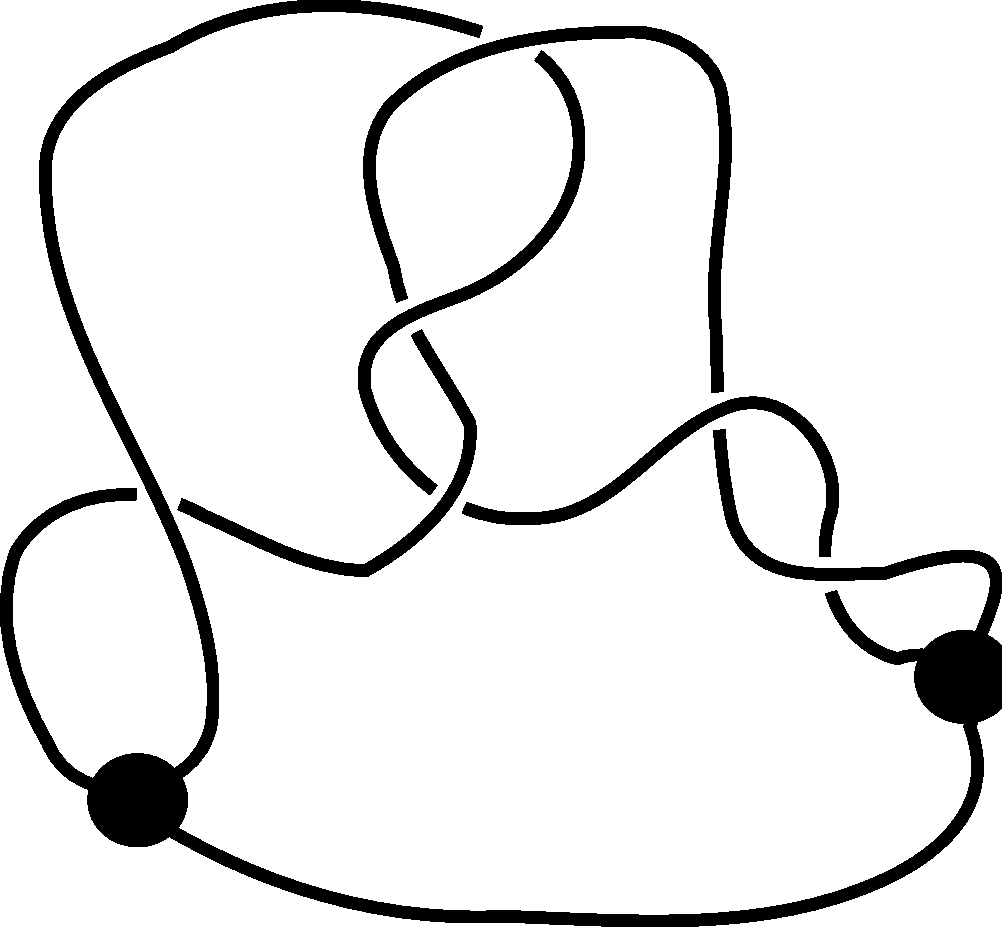
\includegraphics[scale=0.2]{knot_01_1.pdf} &
       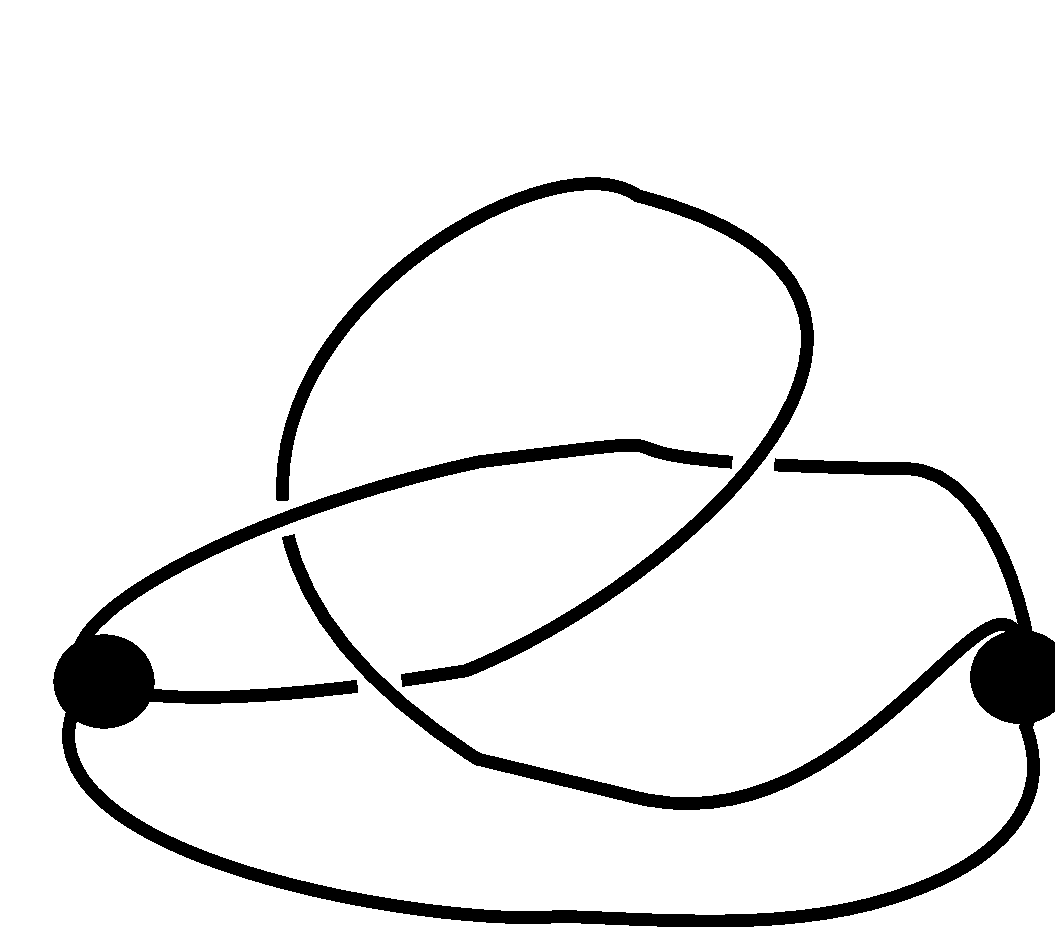
\includegraphics[scale=0.2]{knot_01_7.pdf}\\
       f(G) & g(G)
      \end{matrix}
      \end{equation}

      \dotfill


      \begin{align}
       f(G) & \Rightarrow
       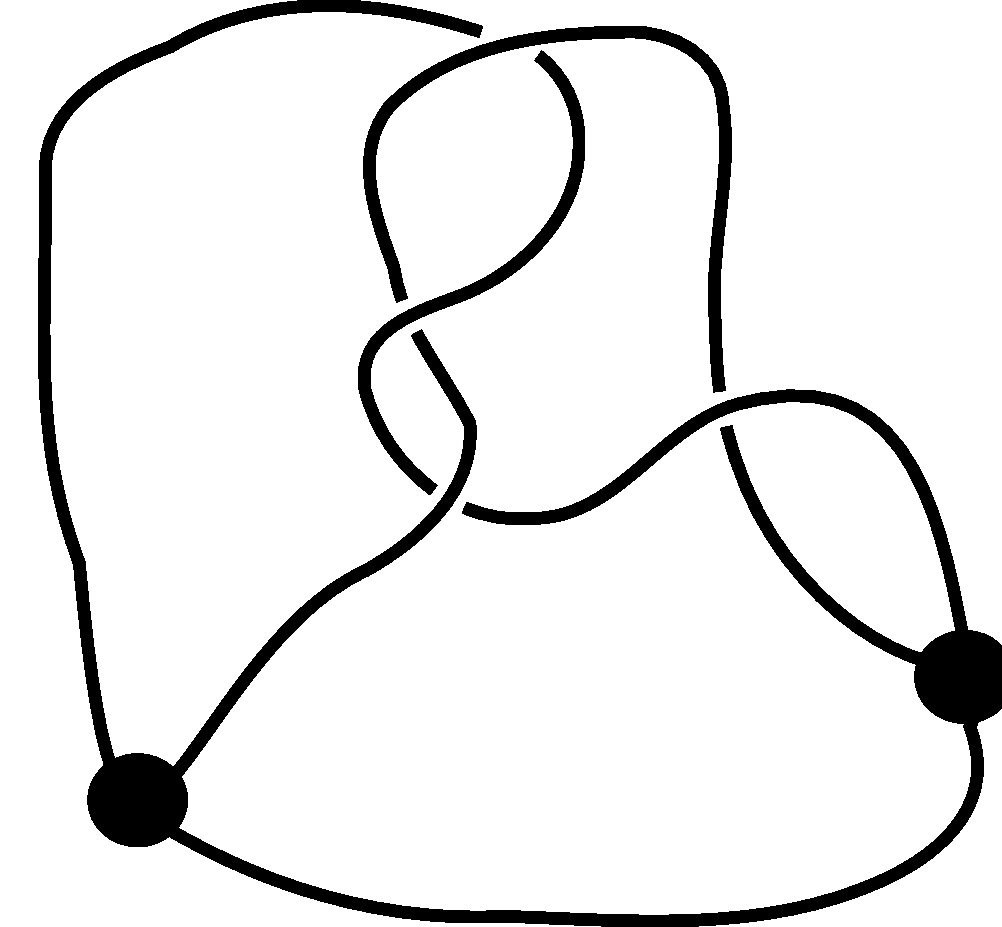
\includegraphics[scale=0.2]{knot_01_2.pdf}
       & \Rightarrow 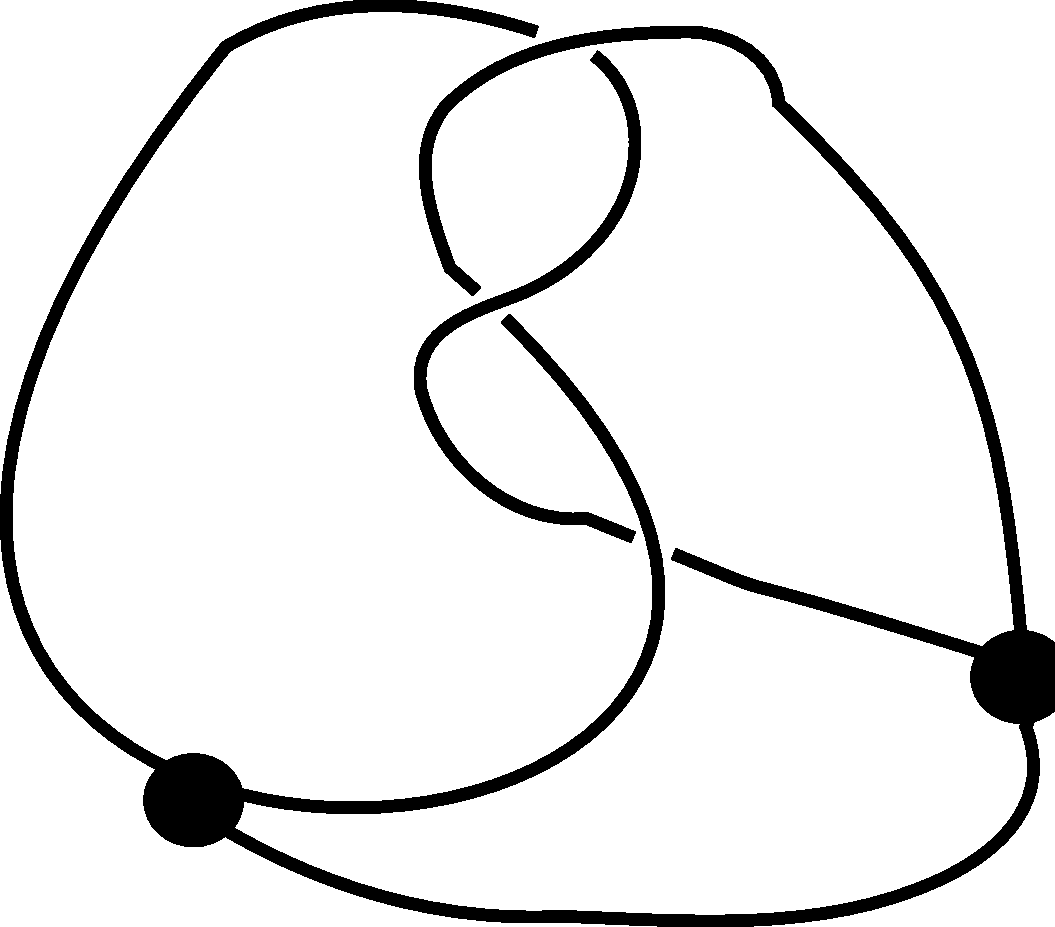
\includegraphics[scale=0.2]{knot_01_3.pdf}\\
       & \Rightarrow 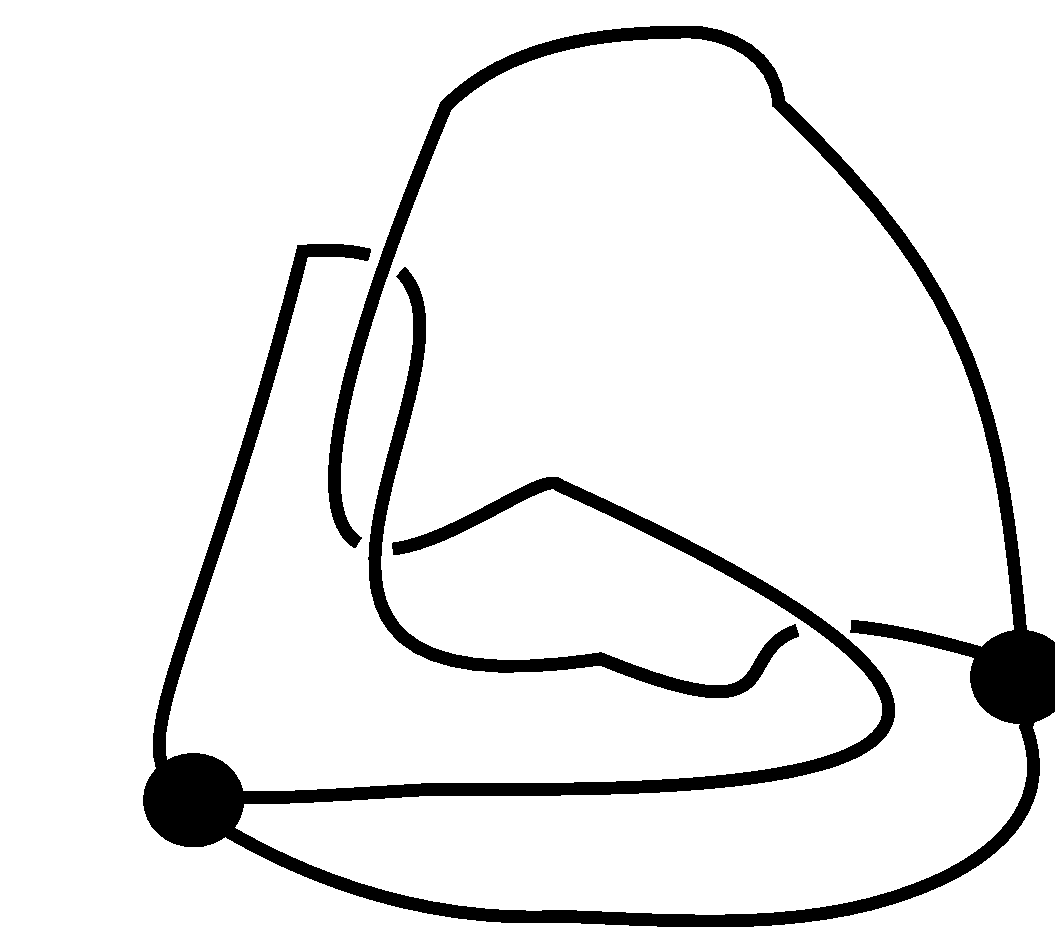
\includegraphics[scale=0.2]{knot_01_4.pdf}
       & \Rightarrow 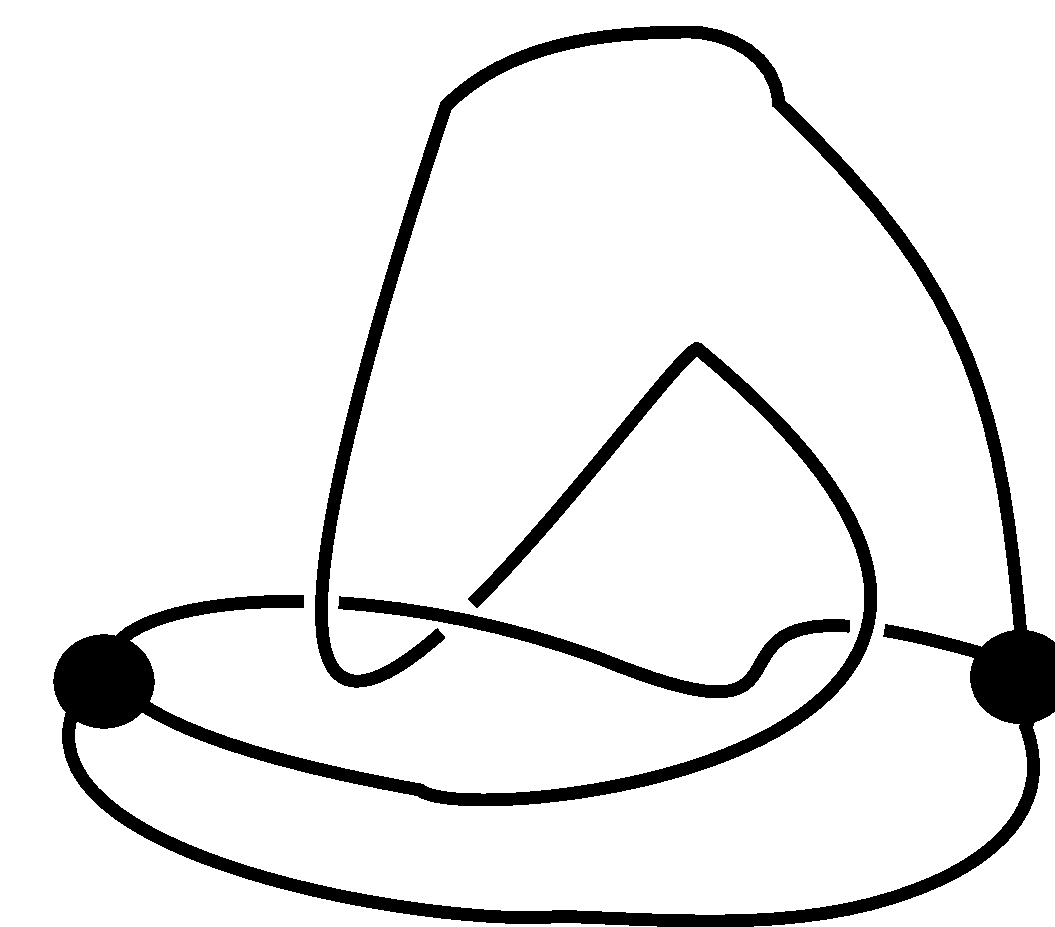
\includegraphics[scale=0.2]{knot_01_5.pdf}\\
       & \Rightarrow 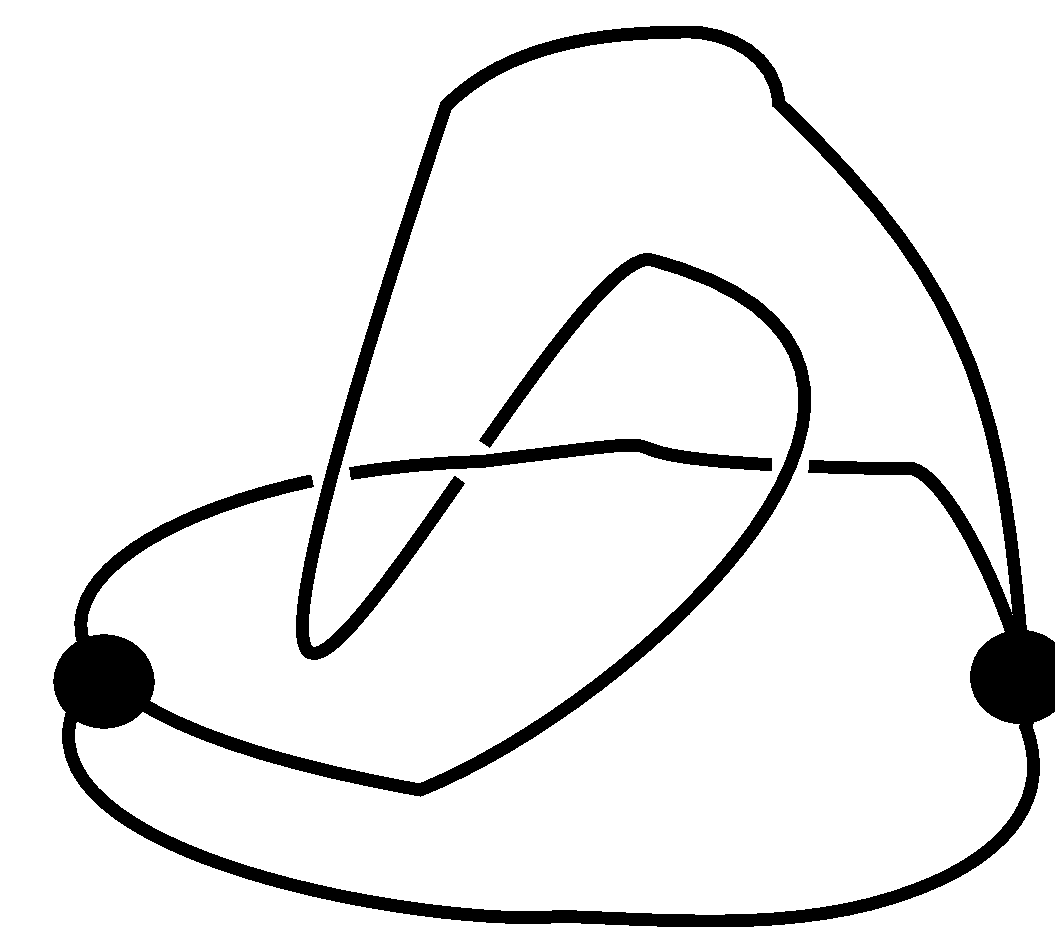
\includegraphics[scale=0.2]{knot_01_6.pdf}
       & \Rightarrow g(G)
      \end{align}



      \hrulefill

 \item
      次の空間グラフ$f(G),g(G)$は互いに同型であることを確かめよ。
      \begin{equation}
      \begin{matrix}
       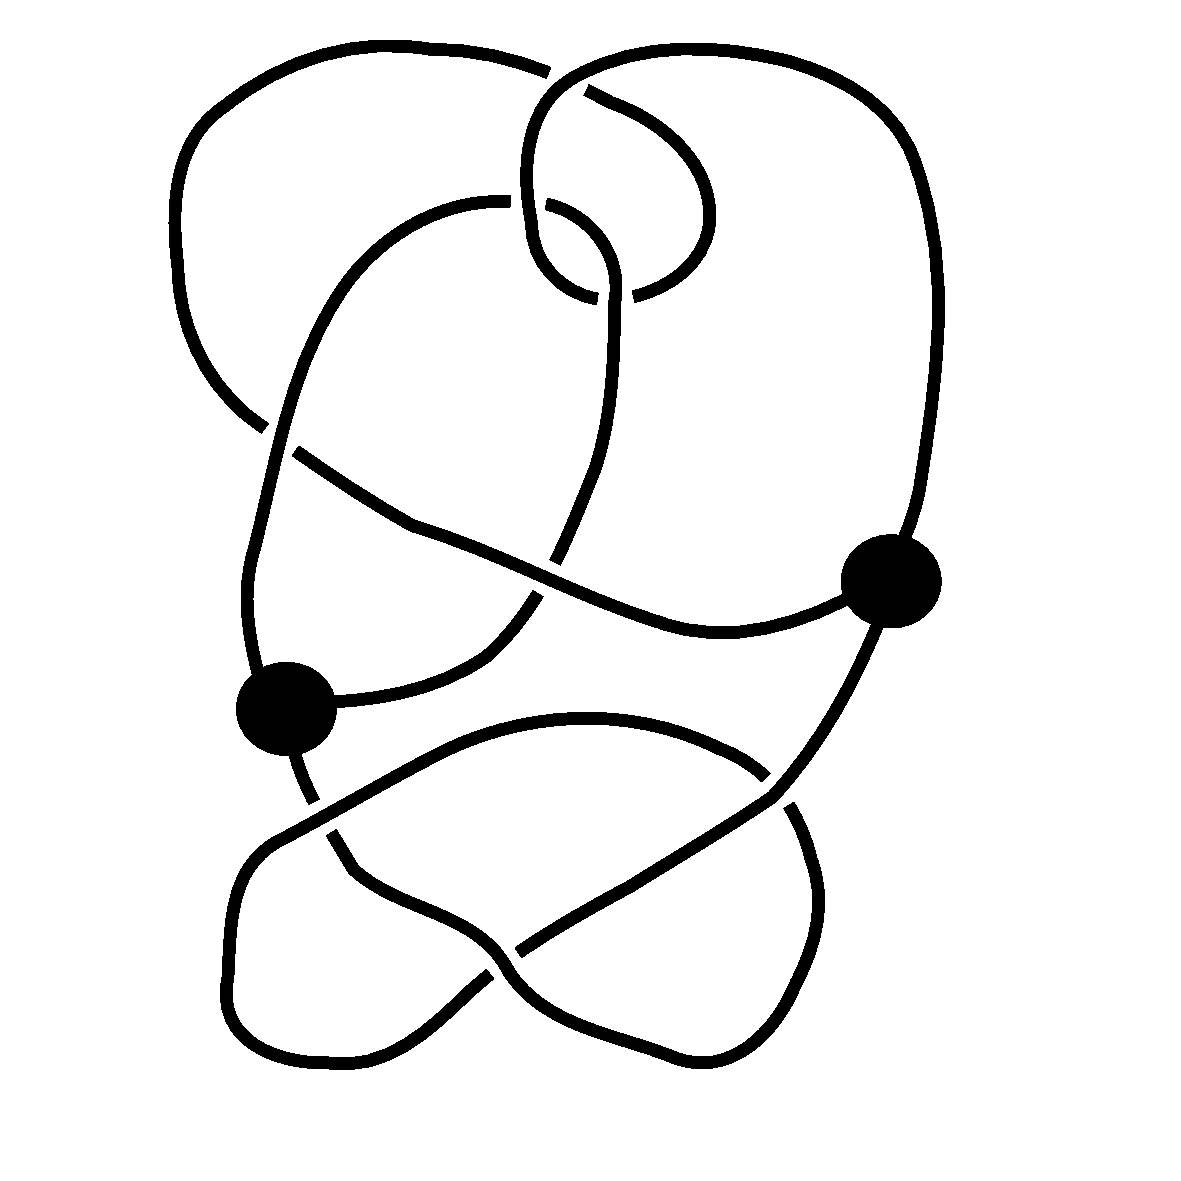
\includegraphics[scale=0.2]{knot_02_1.pdf} &
       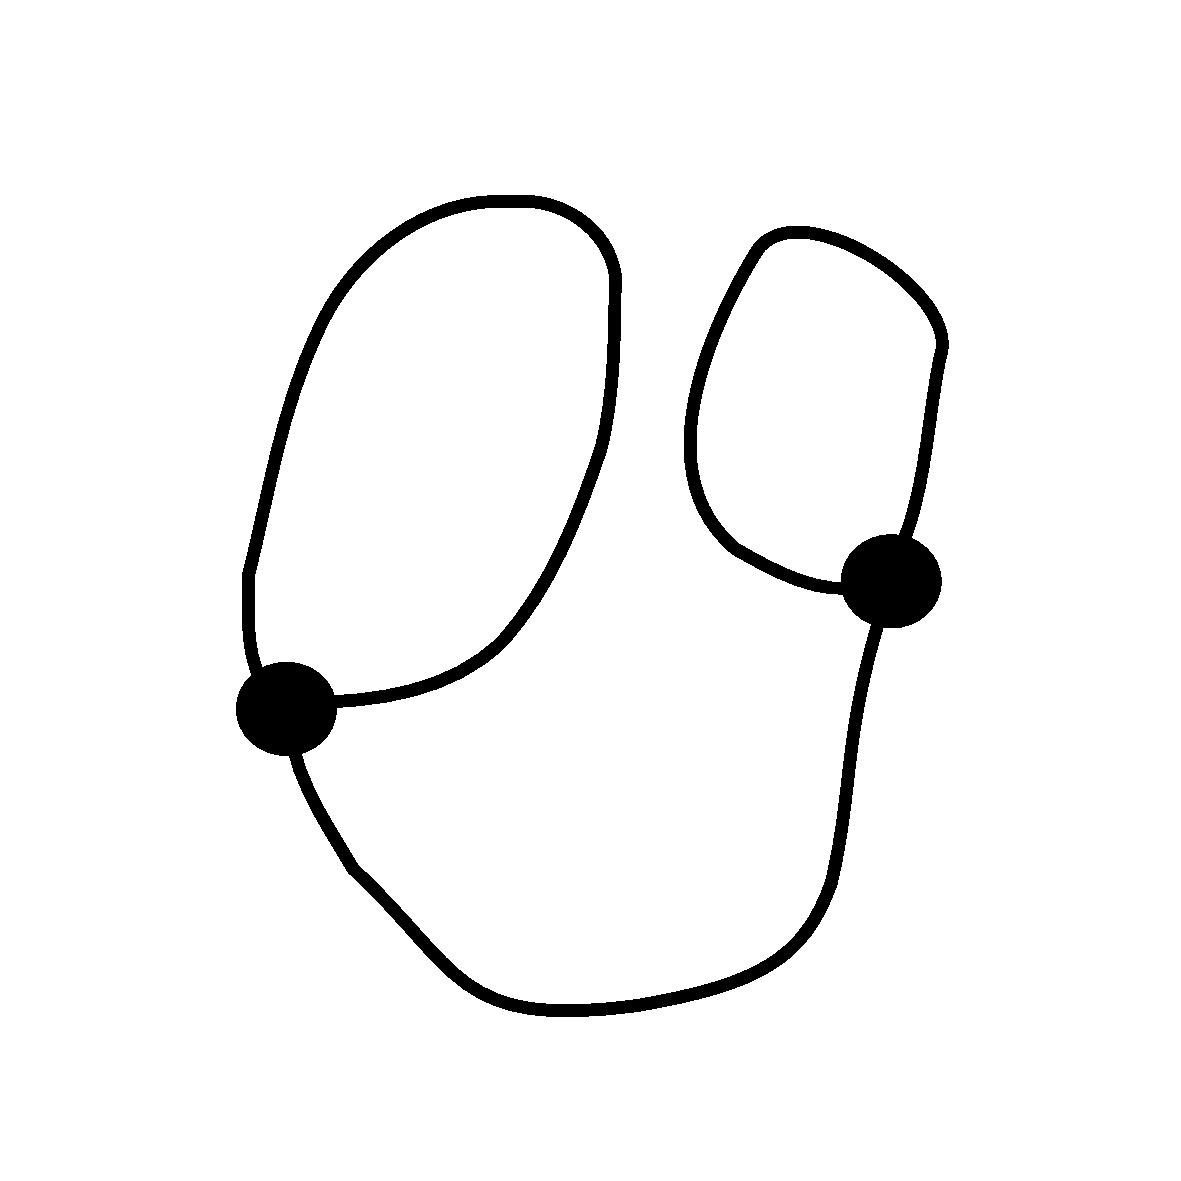
\includegraphics[scale=0.2]{knot_02_5.pdf}\\
       f(G) & g(G)
      \end{matrix}
      \end{equation}


      \dotfill


      \begin{align}
       f(G) & \Rightarrow
       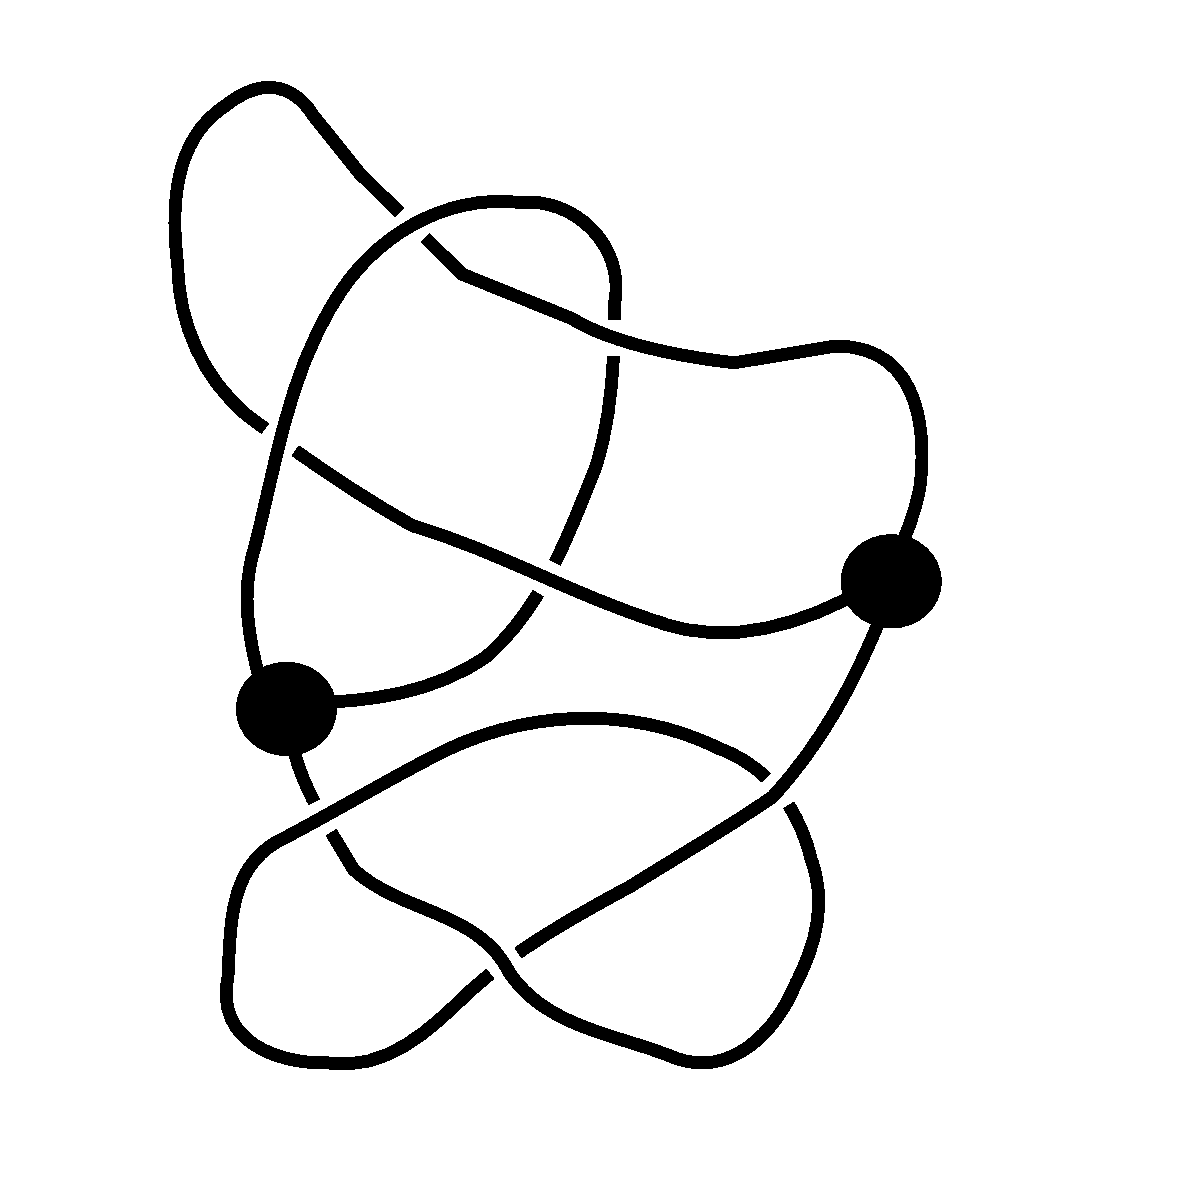
\includegraphics[scale=0.2]{knot_02_2.pdf}
       & \Rightarrow 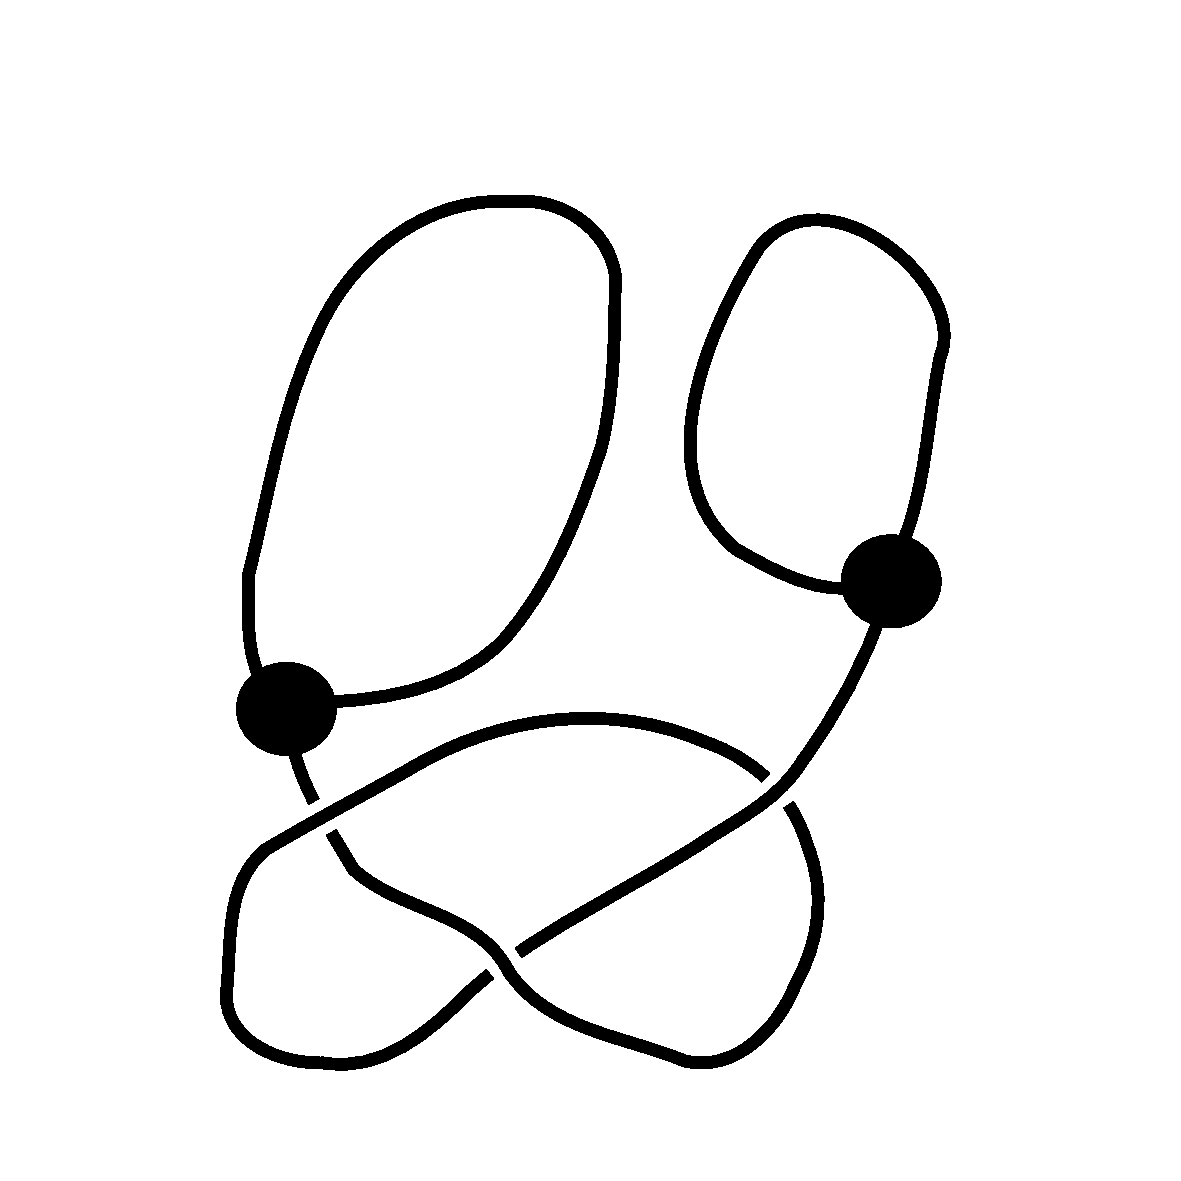
\includegraphics[scale=0.2]{knot_02_3.pdf}\\
       & \Rightarrow 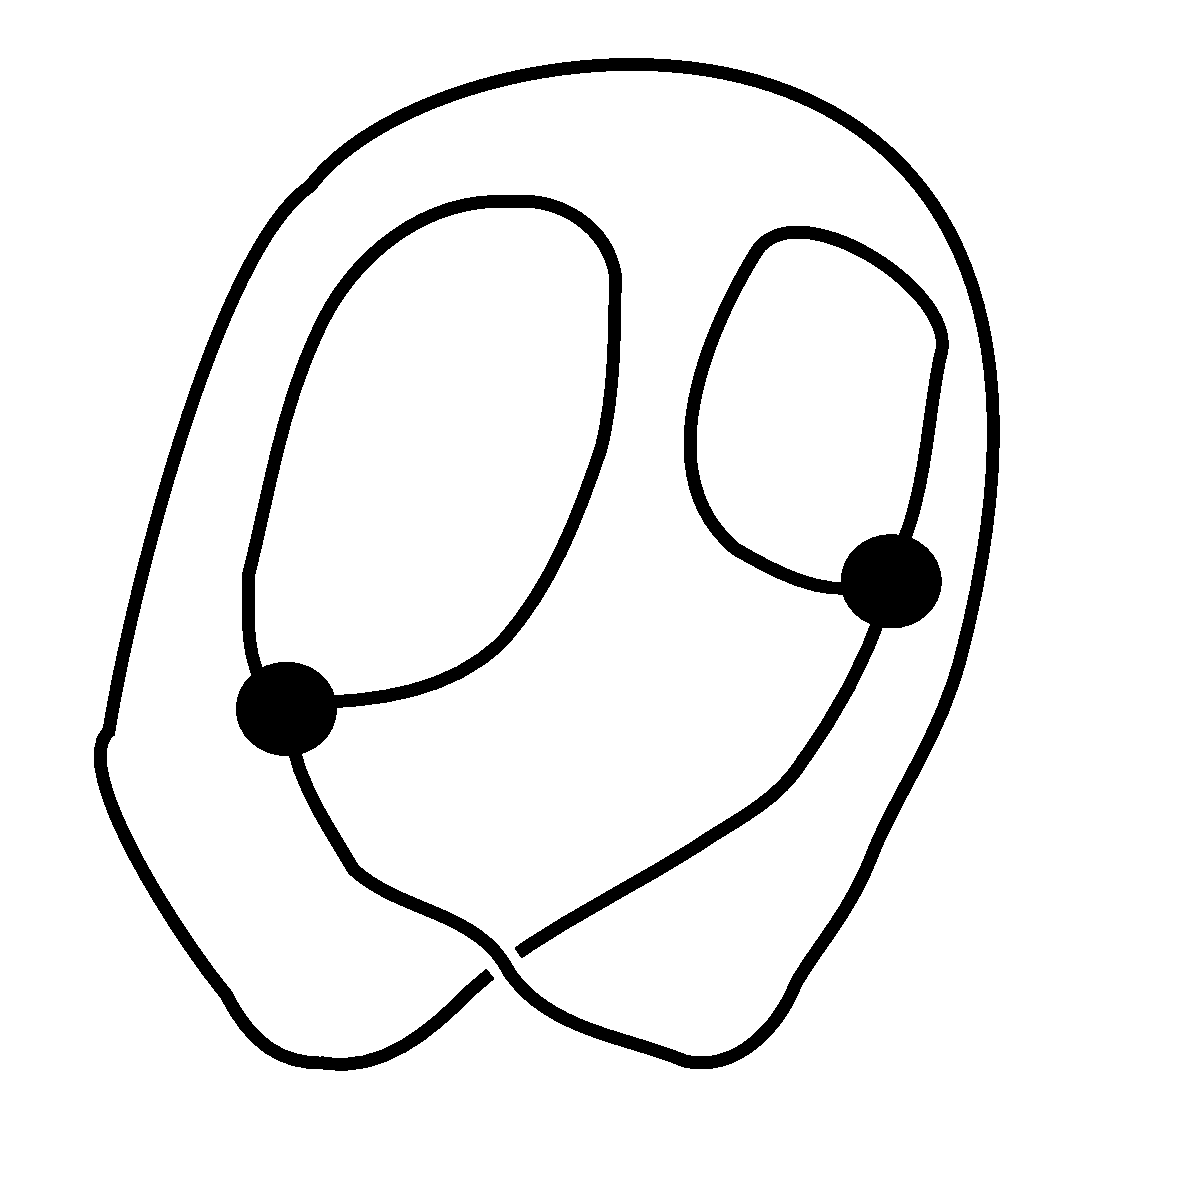
\includegraphics[scale=0.2]{knot_02_4.pdf}
       & \Rightarrow g(G)
      \end{align}


      \hrulefill



 \item
      空間グラフの同型関係$\cong$について、
      以下が成り立つことをそれぞれ示せ。
      \begin{enumerate}
       \item
            空間グラフ$f(G)$に対し、$f(G) \cong f(G)$

            \dotfill

            \begin{equation}
             \Phi : \mathbb{R}^{3}\times [0,1] \to \mathbb{R}^{3}\times [0,1]
            \end{equation}

            写像$\Phi$を恒等写像とすると
            $\Phi(f(G))=f(G)$である。

            \hrulefill

       \item
            空間グラフ$f(G),g(G)$に対し、
            $f(G) \cong g(G)$ならば$g(G) \cong f(G)$

            \dotfill

            $f(G) \cong g(G)$
            であるので、
            同相写像$\Phi$が存在し、
            $\Phi(f(G))=g(G)$である。

            $\Phi$は同相写像なので、
            $X \circ \Phi = \Phi \circ X =id$となる
            同相写像$X$が存在する。

            この$X$により、
            $X(g(G)) = f(G)$であるので、
            $g(G) \cong f(G)$である。

            \hrulefill

       \item
            空間グラフ$f(G),g(G),h(G)$に対し、
            $f(G) \cong g(G)$ かつ $g(G) \cong h(G)$ならば
            $f(G) \cong h(G)$

            \dotfill

            \begin{gather}
             \Phi : \mathbb{R}^{3}\times [0,1] \to \mathbb{R}^{3}\times [0,1]\\
             X : \mathbb{R}^{3}\times [0,1] \to \mathbb{R}^{3}\times [0,1]
            \end{gather}

            $f(G) \cong g(G)$ より
            同相写像$\Phi$が存在し、
            $\Phi(f(G))=g(G)$である。
            
            また、$g(G) \cong h(G)$より
            同相写像$X$が存在し、
            $X(g(G))=h(G)$である。

            $\Phi,X$が同相写像であるので、
            その合成写像$X\circ \Phi$も同相写像であり、
            $X(\Phi(f(G)))=h(G)$である。

            よって、
            $f(G) \cong h(G)$
            である。

            \hrulefill

      \end{enumerate}


 \item
      $X,Y,Z$を位相空間とし、
      $\varphi:X\to Y,\; \psi:Y\to Z$をそれぞれ写像とするとき、
      合成写像$\psi\circ\varphi:X\to Z$について、
      以下の問いに答えよ。
      \begin{enumerate}
       \item
            $\varphi,\,\psi$がともに全単射ならば、
            $\psi\circ\varphi$も全単射であることを示せ。

            \dotfill

            \textbf{全射性}

            $\varphi,\,\psi$がともに全射であるので、
            任意の$y \in Y$に対し$y=\varphi(x)$となる$x\in X$が存在し、
            任意の$z \in Z$に対し$z=\psi(y)$となる$y\in Y$が存在する。

            任意の$z \in Z$に対し$z=\psi(y)$となる$y\in Y$が存在するので、
            この$y\in Y$について$y=\varphi(x)$となる$x\in X$が存在する。

            つまり、${}^{\forall}z\in Z$に対し、
            $z=\psi\circ\varphi(x)$となる$x\in X$が存在する。

            よって、
            $\psi\circ\varphi$は全射である。

            \textbf{単射性}

            $\varphi,\,\psi$がともに単射である。

            $y_{1},y_{2}\in Y$に対し、
            $\psi(y_{1})=\psi(y_{2})$であれば$y_{1}=y_{2}$である。

            $\varphi$は全射であるので、
            $y_{1}=\varphi(x_{1}),\;y_{2}=\varphi(x_{2})$
            となる$x_{1},x_{2}\in X$が存在する。
            $\varphi$は単射であるので、
            $x_{1}=x_{2}$である。

            つまり、
            $\psi(\varphi(x_{1}))=\psi(\varphi(x_{2}))$であれば
            $x_{1}=x_{2}$である。

            よって、
            $\psi\circ\varphi$は単射である。

            この2つより
            $\psi\circ\varphi$は単全射である。

            \hrulefill

       \item
            $\varphi,\,\psi$がともに連続写像ならば、
            $\psi\circ\varphi$も連続写像であることを示せ。

            \dotfill

            $\varphi,\,\psi$が連続写像であるので、
            任意の開集合$U_{Y}\subset Y,\; U_{Z}\subset Z$に対して、
            $\varphi^{-1}(U_{Y}),\; \psi^{-1}(U_{Z})$が開集合となる。

            $\psi^{-1}(U_{Z})$が開集合であるので、
            $\varphi^{-1}(\psi^{-1}(U_{Z}))$も開集合となる。

            つまり、
            任意の開集合$U_{Z}\subset Z$に対して、
            $(\varphi^{-1}\circ\psi^{-1})(U_{Z})$も開集合となる。

            $(\varphi^{-1}\circ\psi^{-1})(U_{Z})=(\psi\circ\varphi)^{-1}(U_{Z})$
            であるので、
            写像$\psi\circ\varphi : X\to Z$は連続写像である。

            \hrulefill

       \item
            $\varphi$が$X$から$Y$への同相写像で、
            かつ、
            $\psi$が$Y$から$Z$への同相写像ならば、
            $\psi\circ\varphi$は$X$から$Z$への同相写像となることを示せ。

            \dotfill

            同相写像とは、全単射な連続写像であり、
            その逆写像も連続写像であるものをいう。

            先の問より、$\varphi,\psi$が全単射な連続写像であるので、
            合成写像$\psi\circ\varphi$も全単射な連続写像である。

            また、
            $\varphi^{-1}:Y\to X,\; \psi^{-1}:Z\to Y$も連続写像であるので、
            その合成写像$\varphi^{-1}\circ\psi^{-1}=(\psi\circ\varphi)$も
            連続写像である。

            よって、
            $\psi\circ\varphi$は同相写像である。

            \hrulefill


      \end{enumerate}


 \item
      次の図式が表す結び目$K$は自明であることを確かめよ。
      \begin{center}
       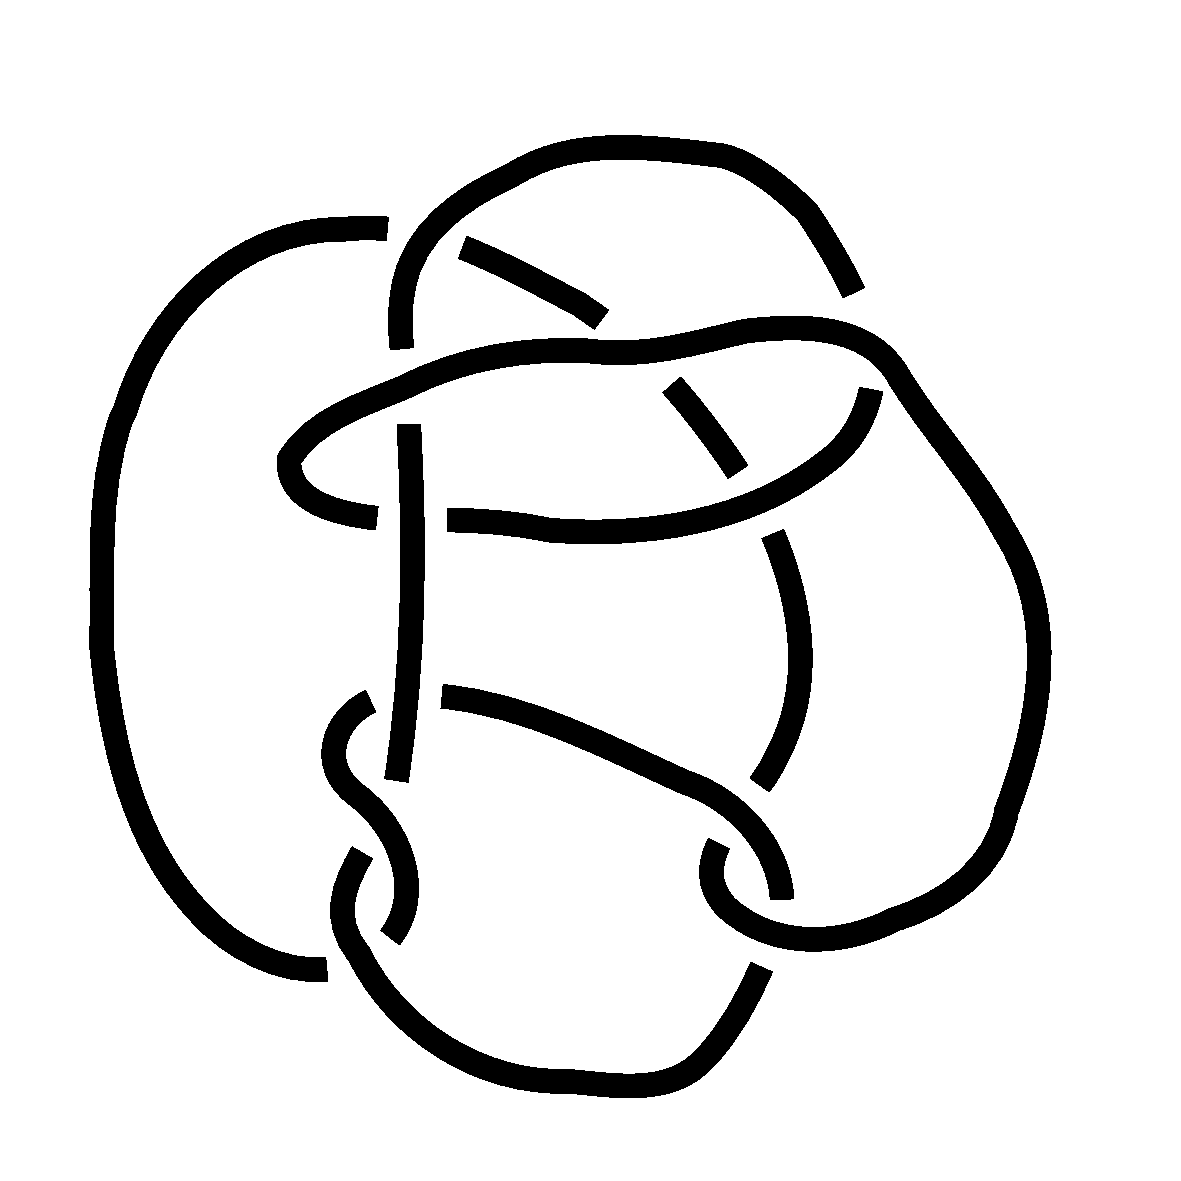
\includegraphics[scale=0.2]{knot_05_01.pdf}
      \end{center}

      \dotfill

      \begin{align}
       K & \Rightarrow
         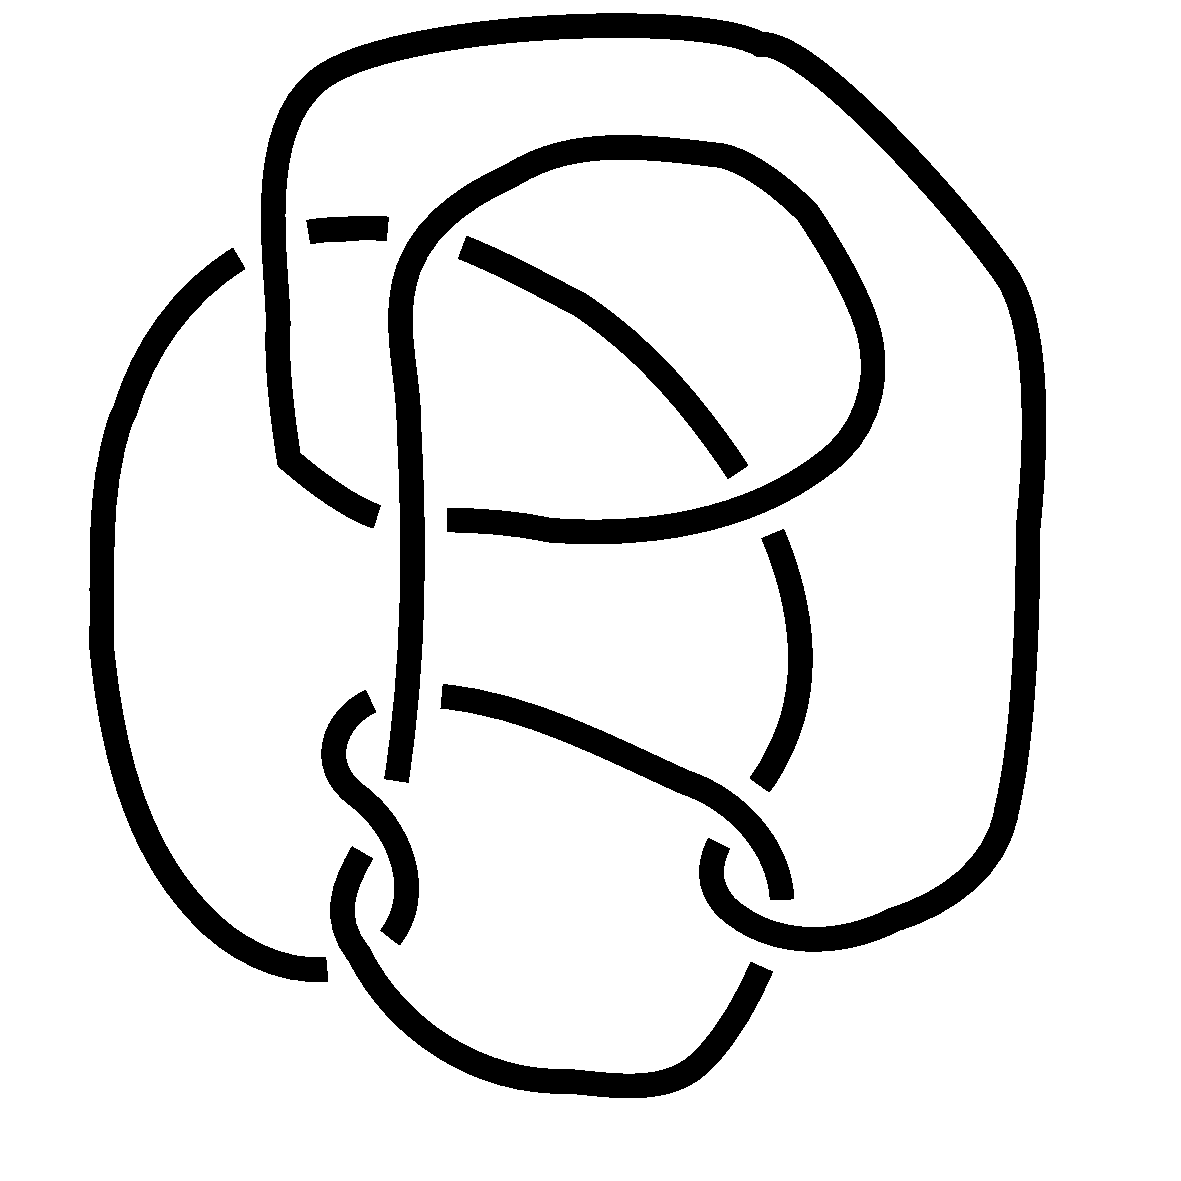
\includegraphics[scale=0.2]{knot_05_02.pdf}
       \Rightarrow 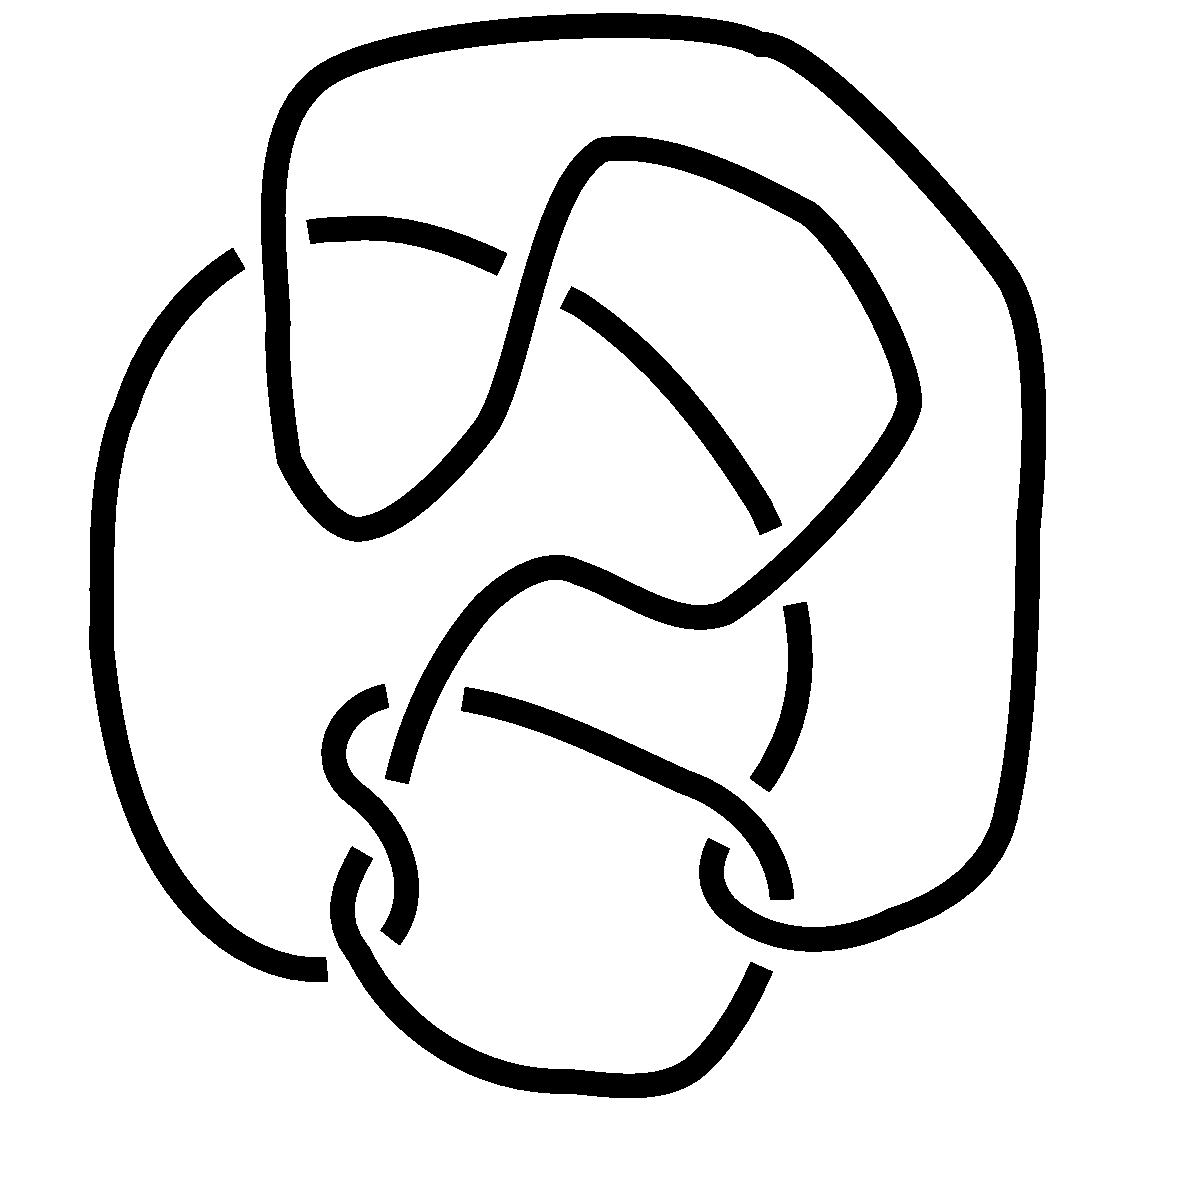
\includegraphics[scale=0.2]{knot_05_03.pdf}
       \Rightarrow 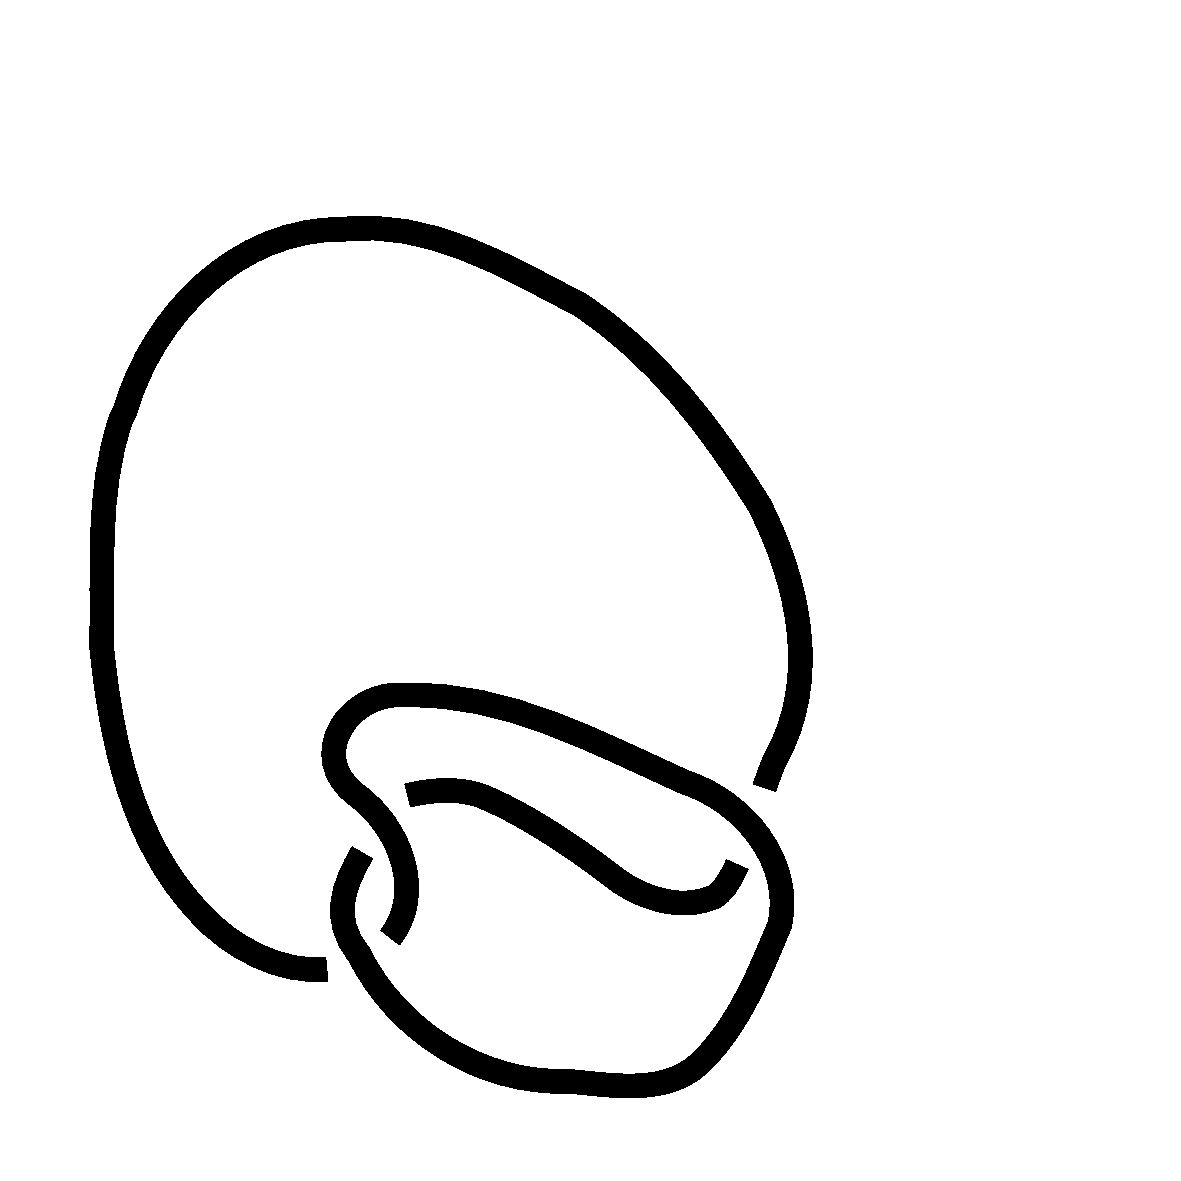
\includegraphics[scale=0.2]{knot_05_04.pdf}\\
       &\Rightarrow 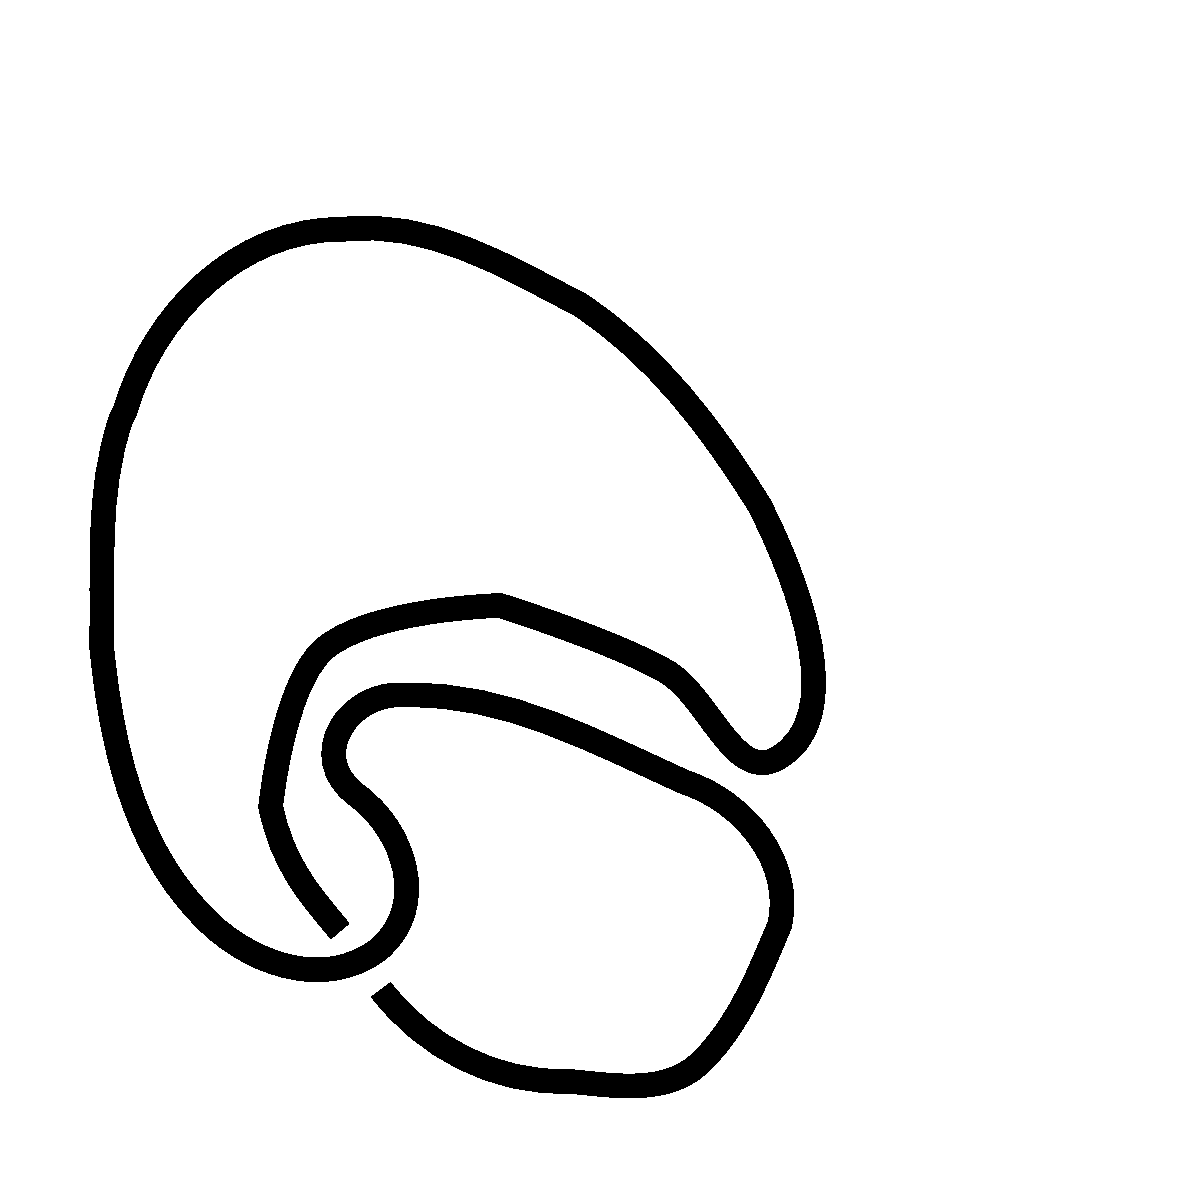
\includegraphics[scale=0.2]{knot_05_05.pdf}
       \Rightarrow 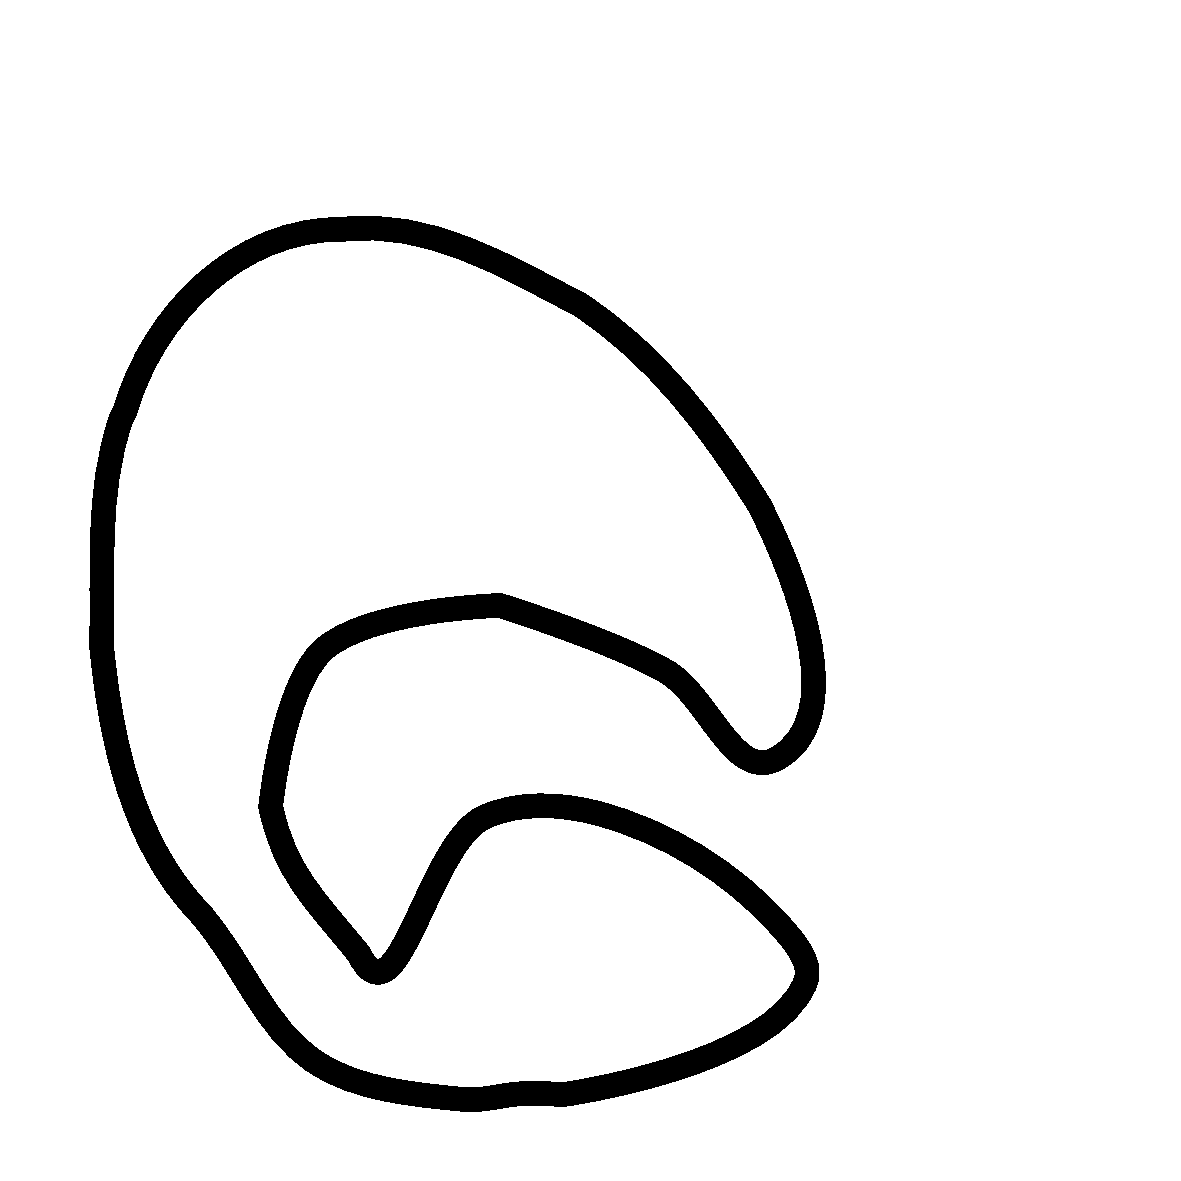
\includegraphics[scale=0.2]{knot_05_06.pdf}
       \Rightarrow 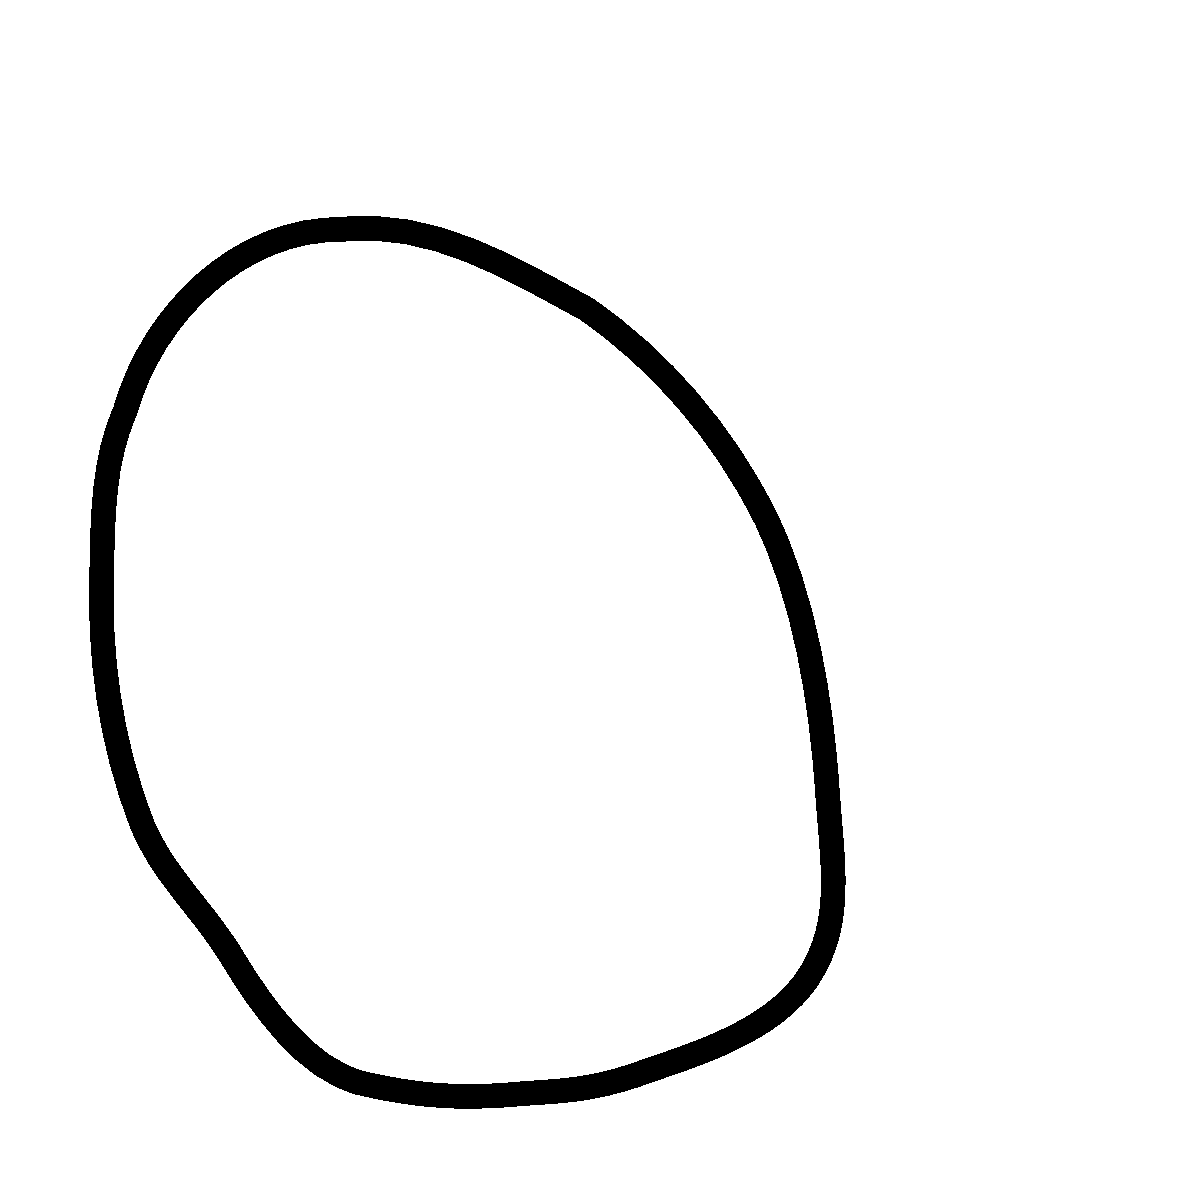
\includegraphics[scale=0.2]{knot_05_07.pdf}
      \end{align}

      \hrulefill

 \item
      次の図式が表す空間グラフ$f(G)$は分離していることを確かめよ。
      \begin{center}
       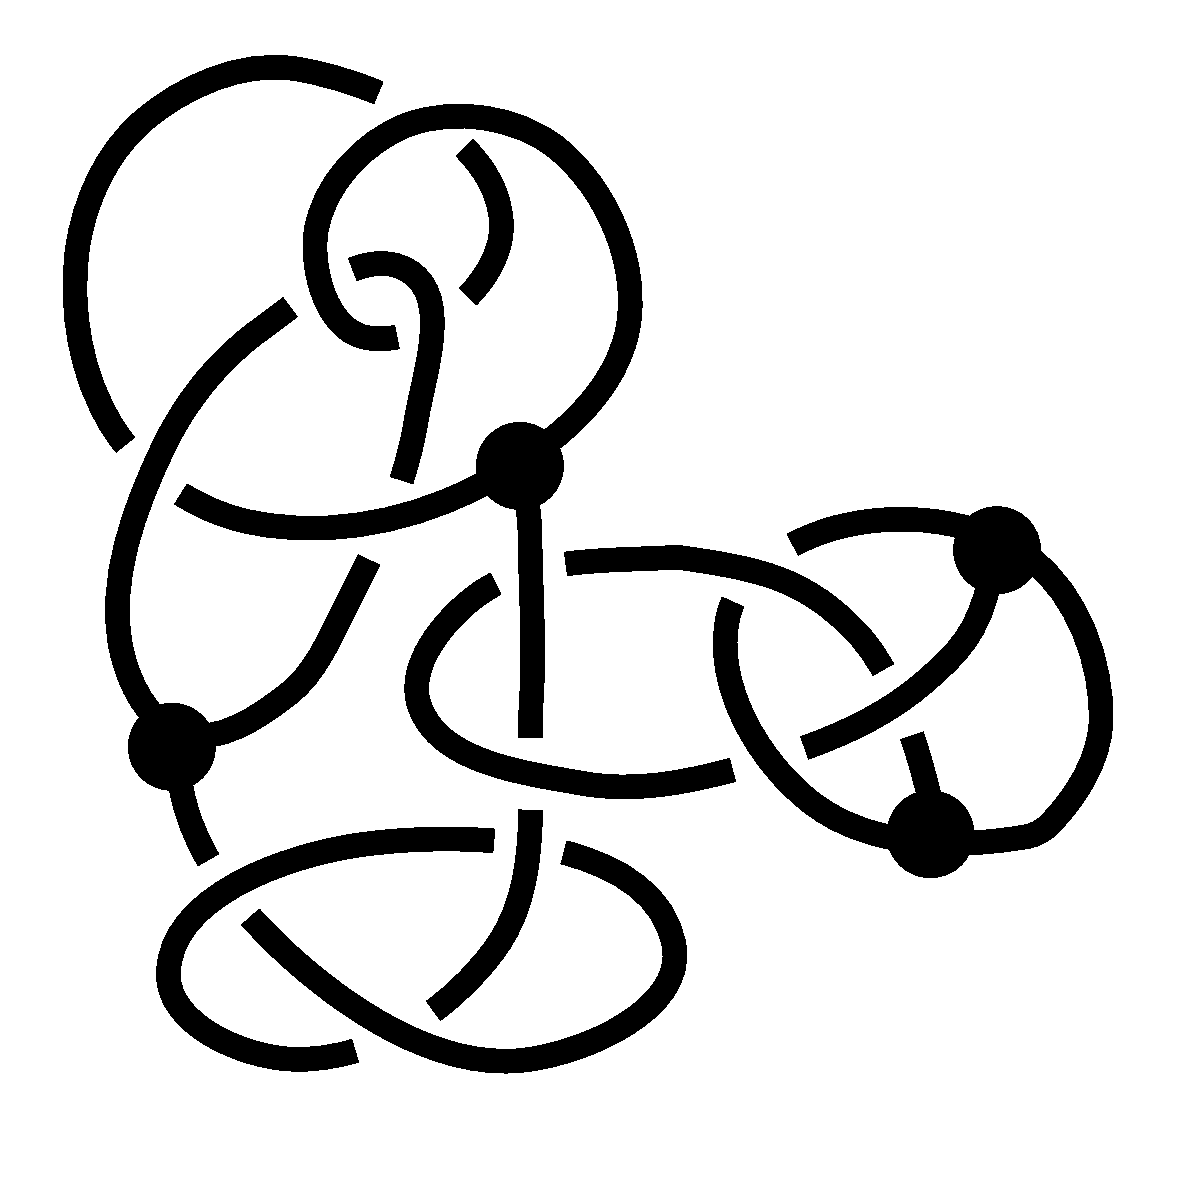
\includegraphics[scale=0.2]{knot_06_01.pdf}
      \end{center}

      \dotfill

      \begin{align}
       f(G) & \Rightarrow
         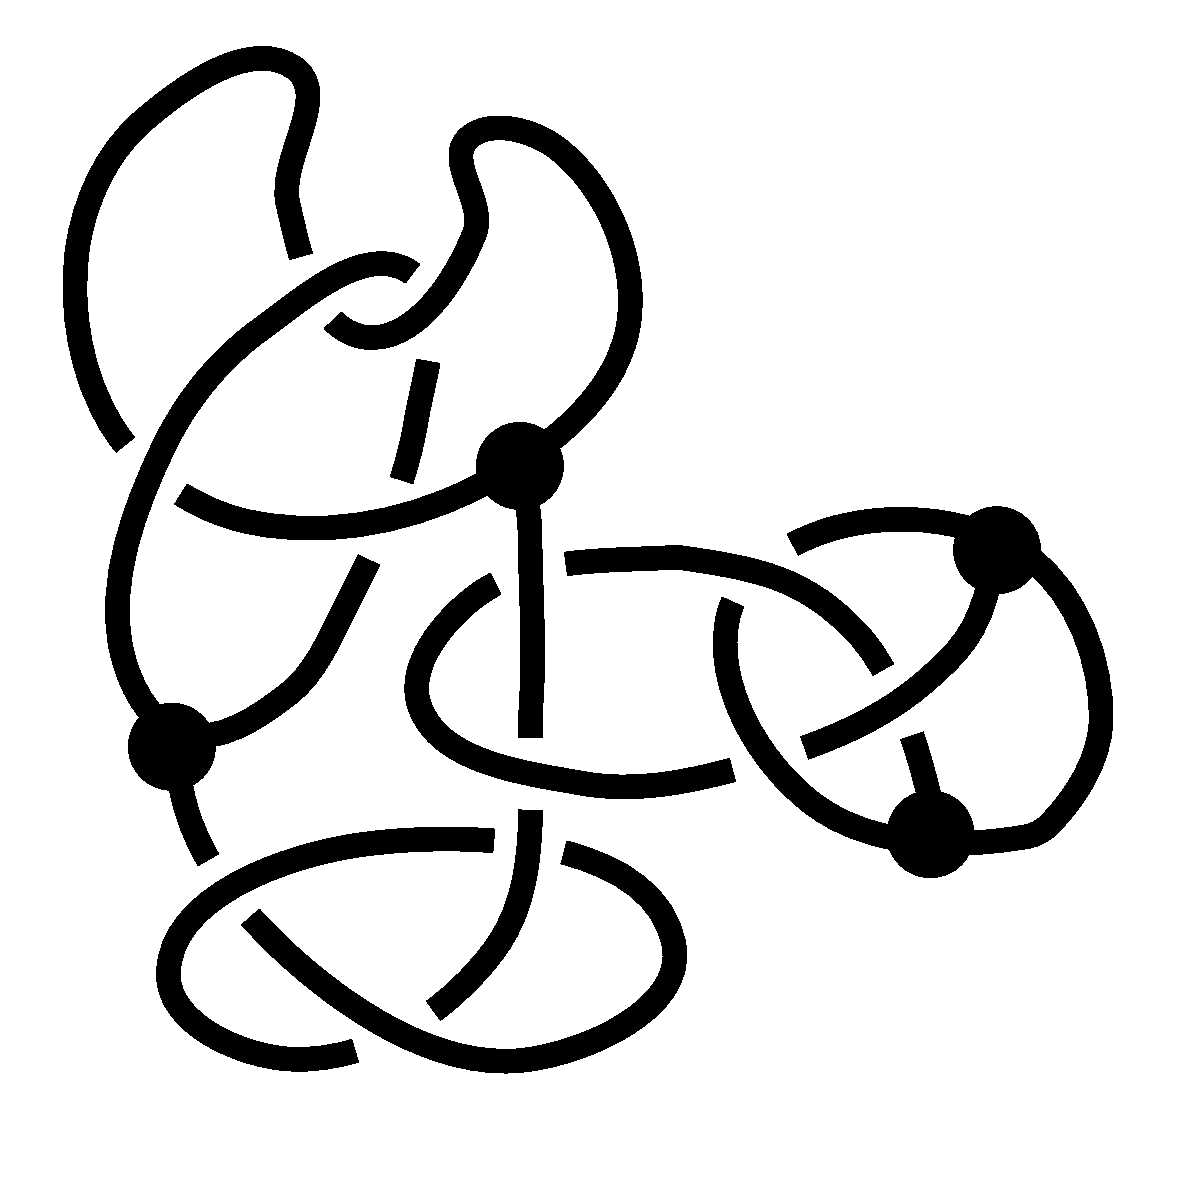
\includegraphics[scale=0.2]{knot_06_02.pdf}
       \Rightarrow 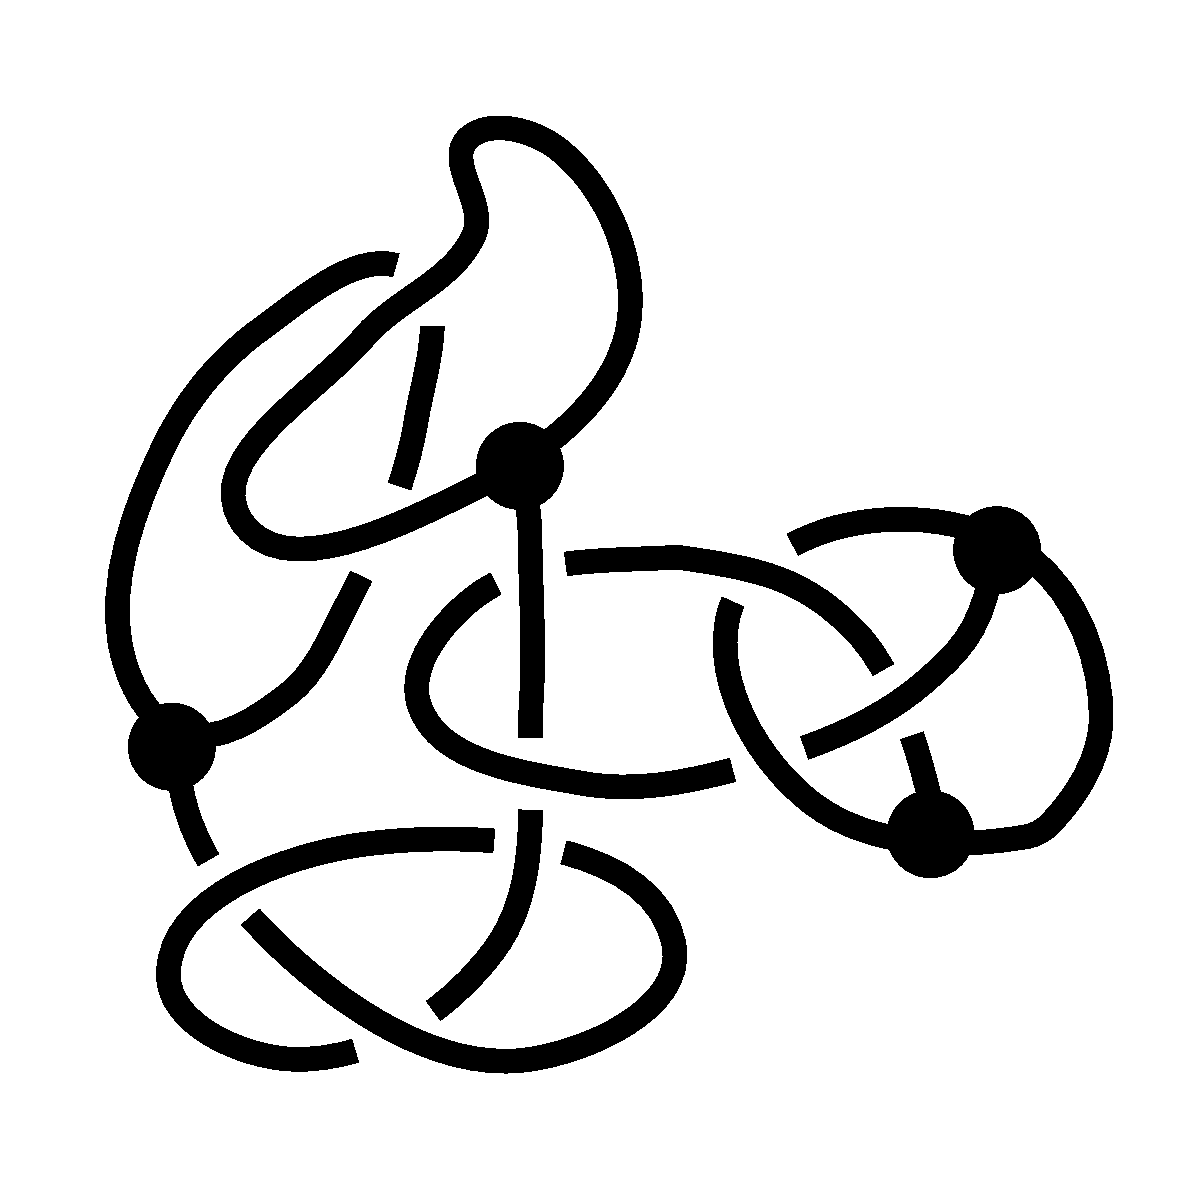
\includegraphics[scale=0.2]{knot_06_03.pdf}\\
       &\Rightarrow 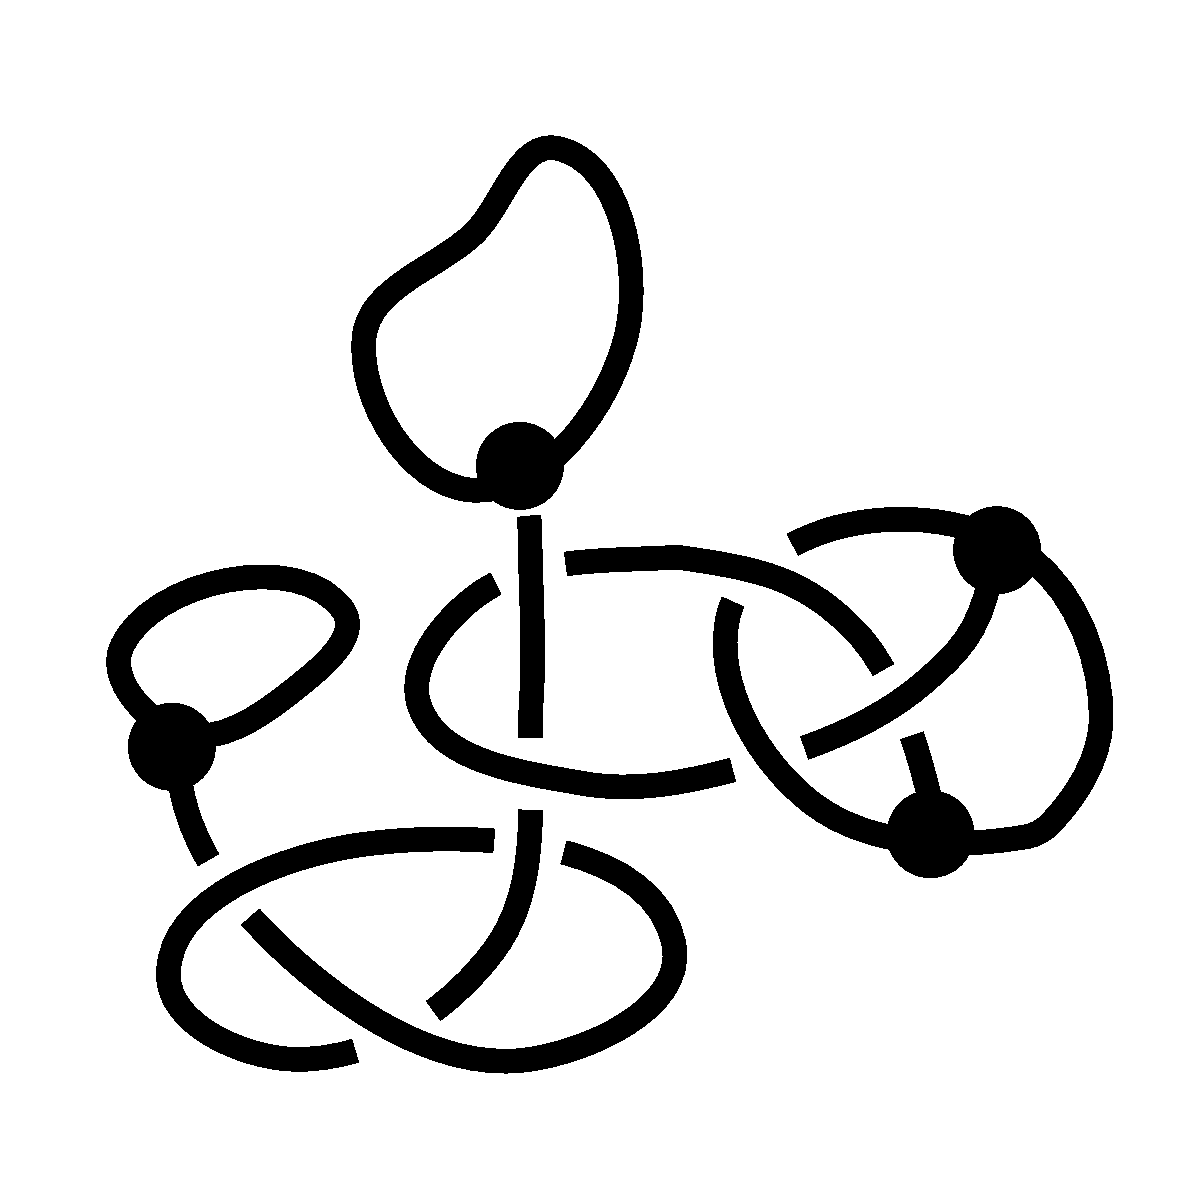
\includegraphics[scale=0.2]{knot_06_04.pdf}
       \Rightarrow 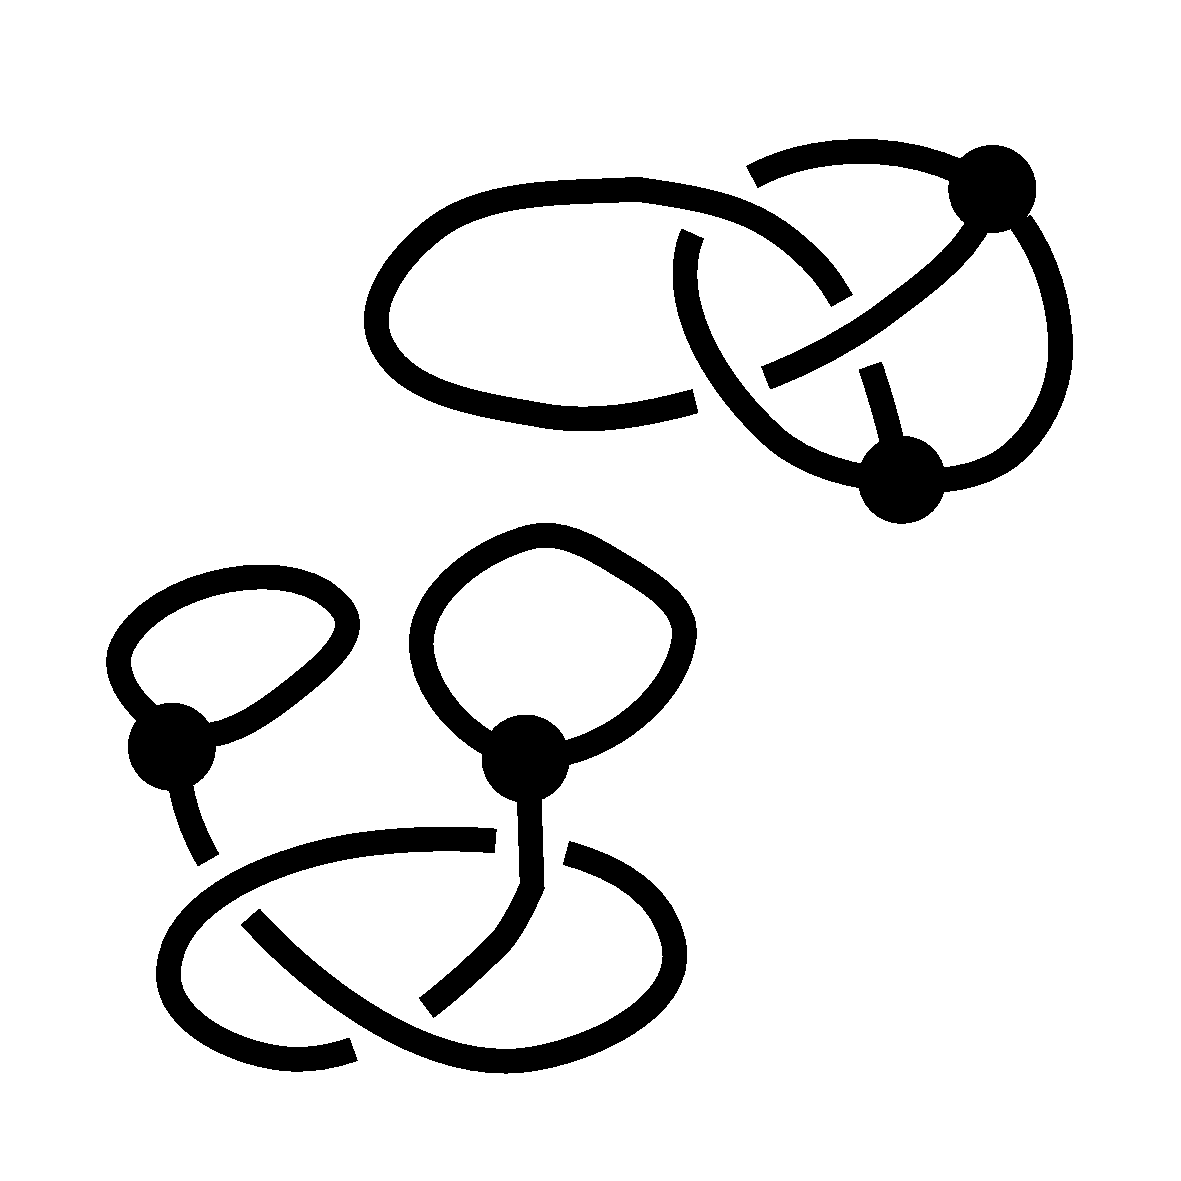
\includegraphics[scale=0.2]{knot_06_05.pdf}
      \end{align}

      \hrulefill


 \item
      $f(G),g(G)$は、
      それぞれ次の図式$\tilde{f}(G),\tilde{g}(G)$
      で表された空間グラフとする。
      この時、
      $\tilde{f}(G)$と$\tilde{g}(G)$の間の
      \ruby{Reidemeister}{ライデマイスター}変形の
      列を具体的に図示せよ。

      \begin{equation}
       \begin{matrix}
        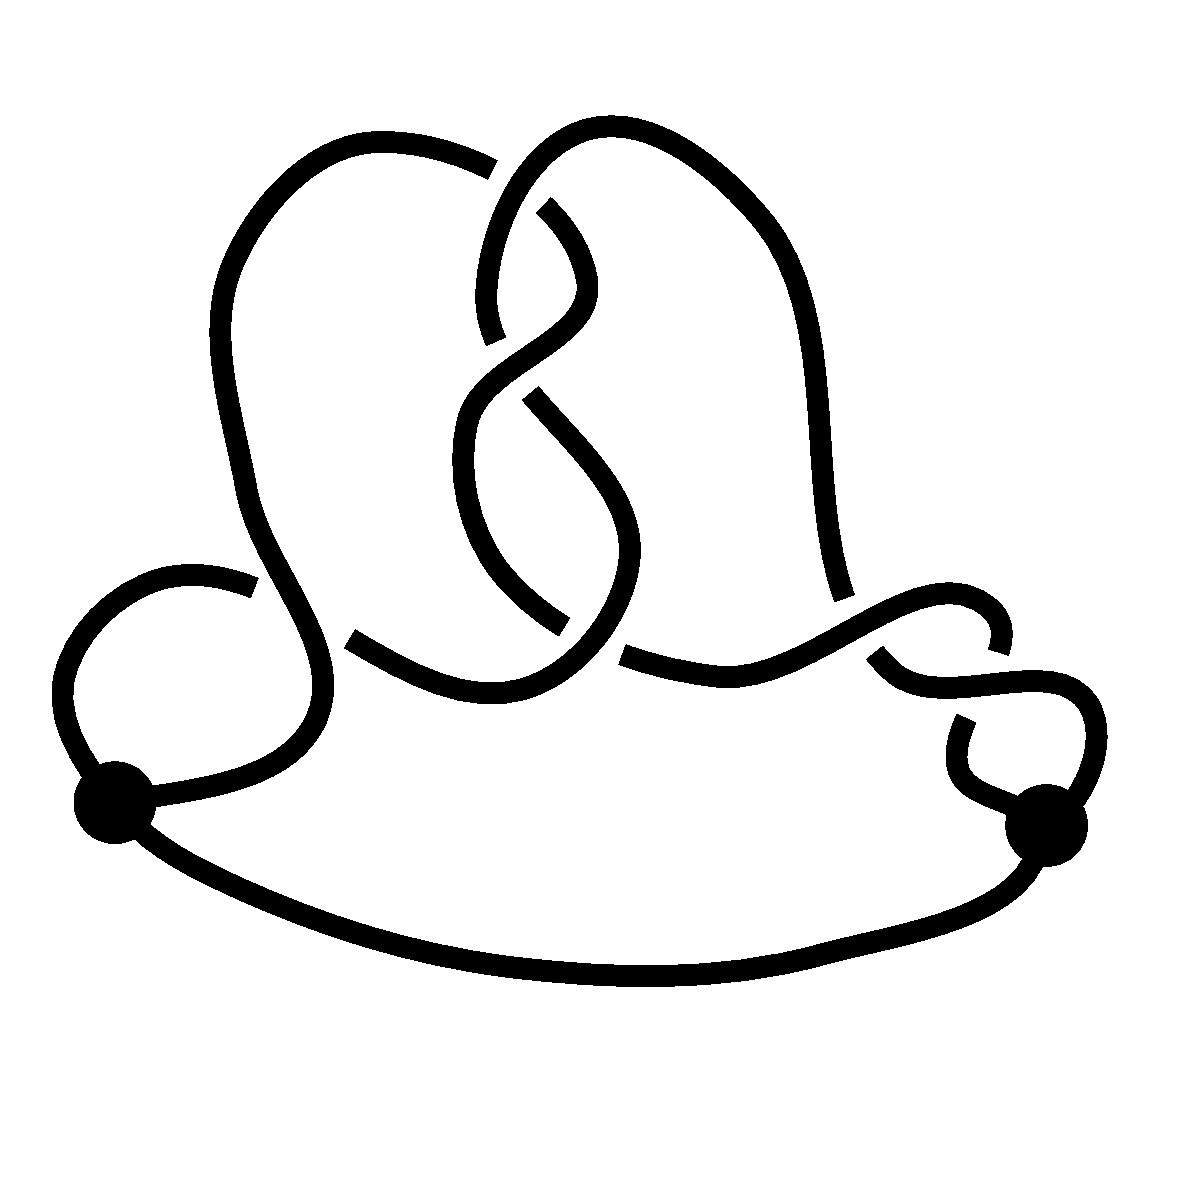
\includegraphics[scale=0.2]{knot_07_01.pdf} &
       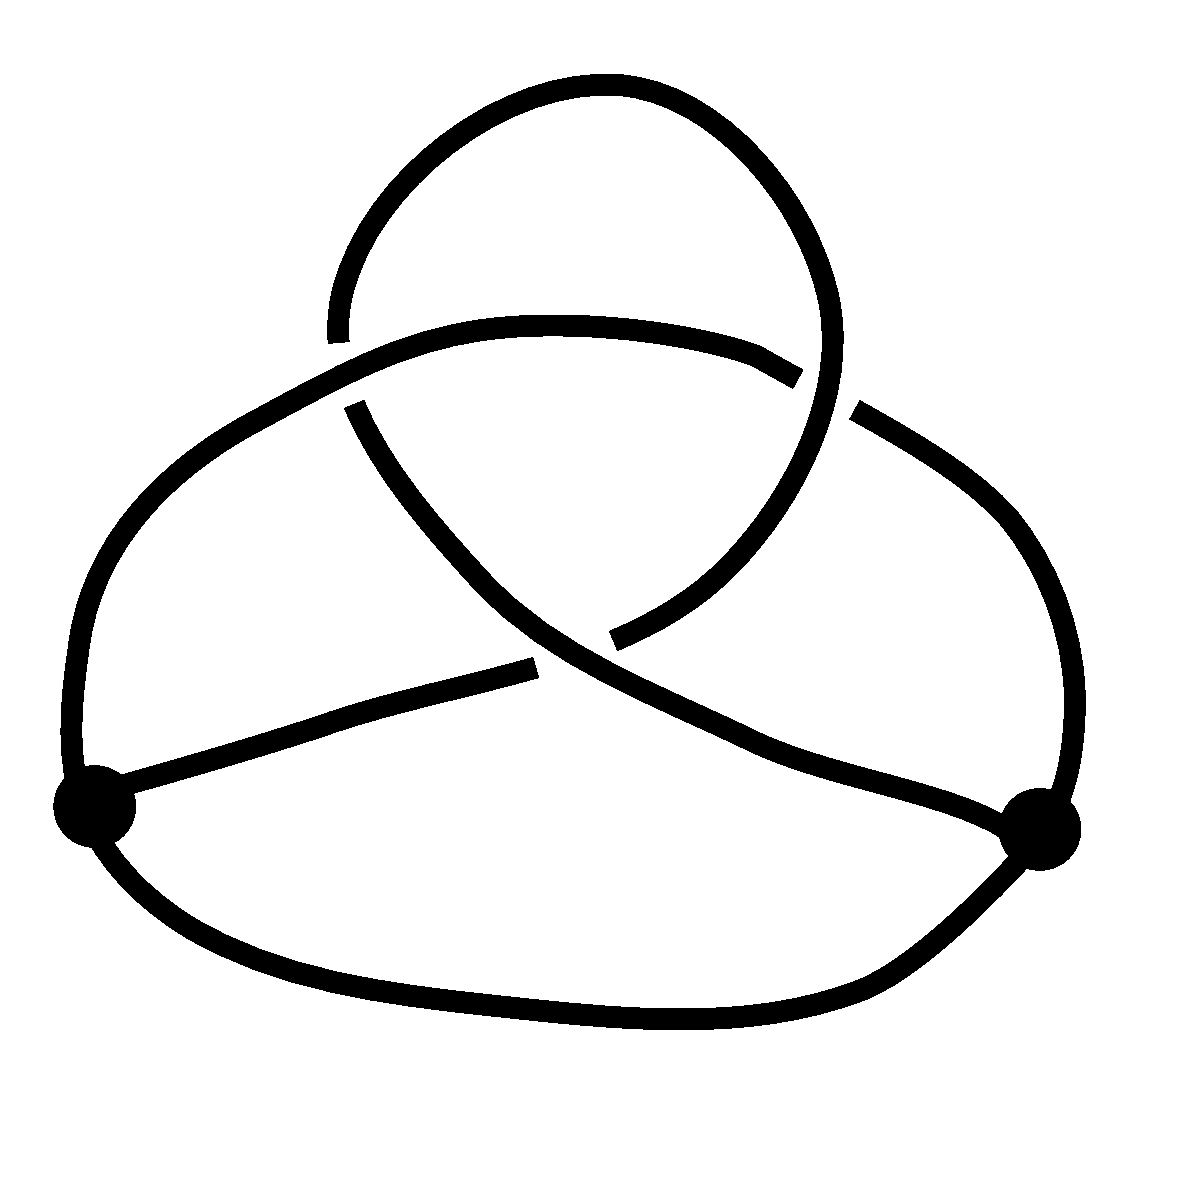
\includegraphics[scale=0.2]{knot_07_13.pdf}\\
       \tilde{f}(G) & \tilde{g}(G)
       \end{matrix}
       \end{equation}


      \dotfill

      \textbf{Reidemeister 変形}

      捻る(R.I)、パスの上下と移動する(R.II)、交点の上下を移動する(R.III)

      \dotfill


       \begin{align}
        \tilde{f}(G)
        & \overset{}{\Rightarrow} 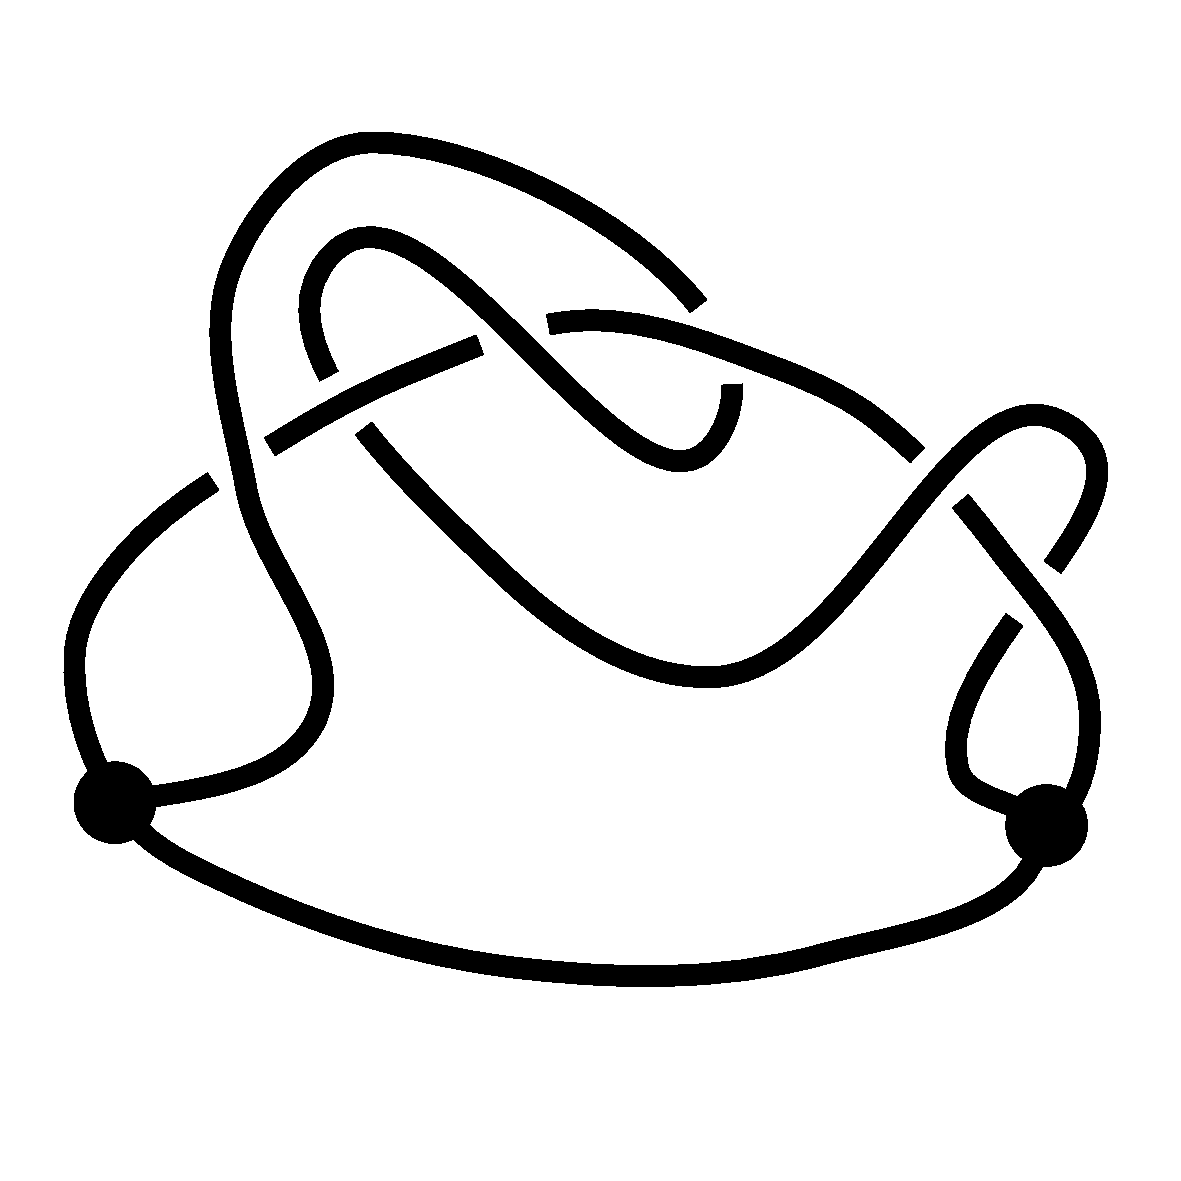
\includegraphics[scale=0.15]{knot_07_02.pdf}
        & \overset{R.II}{\Rightarrow} 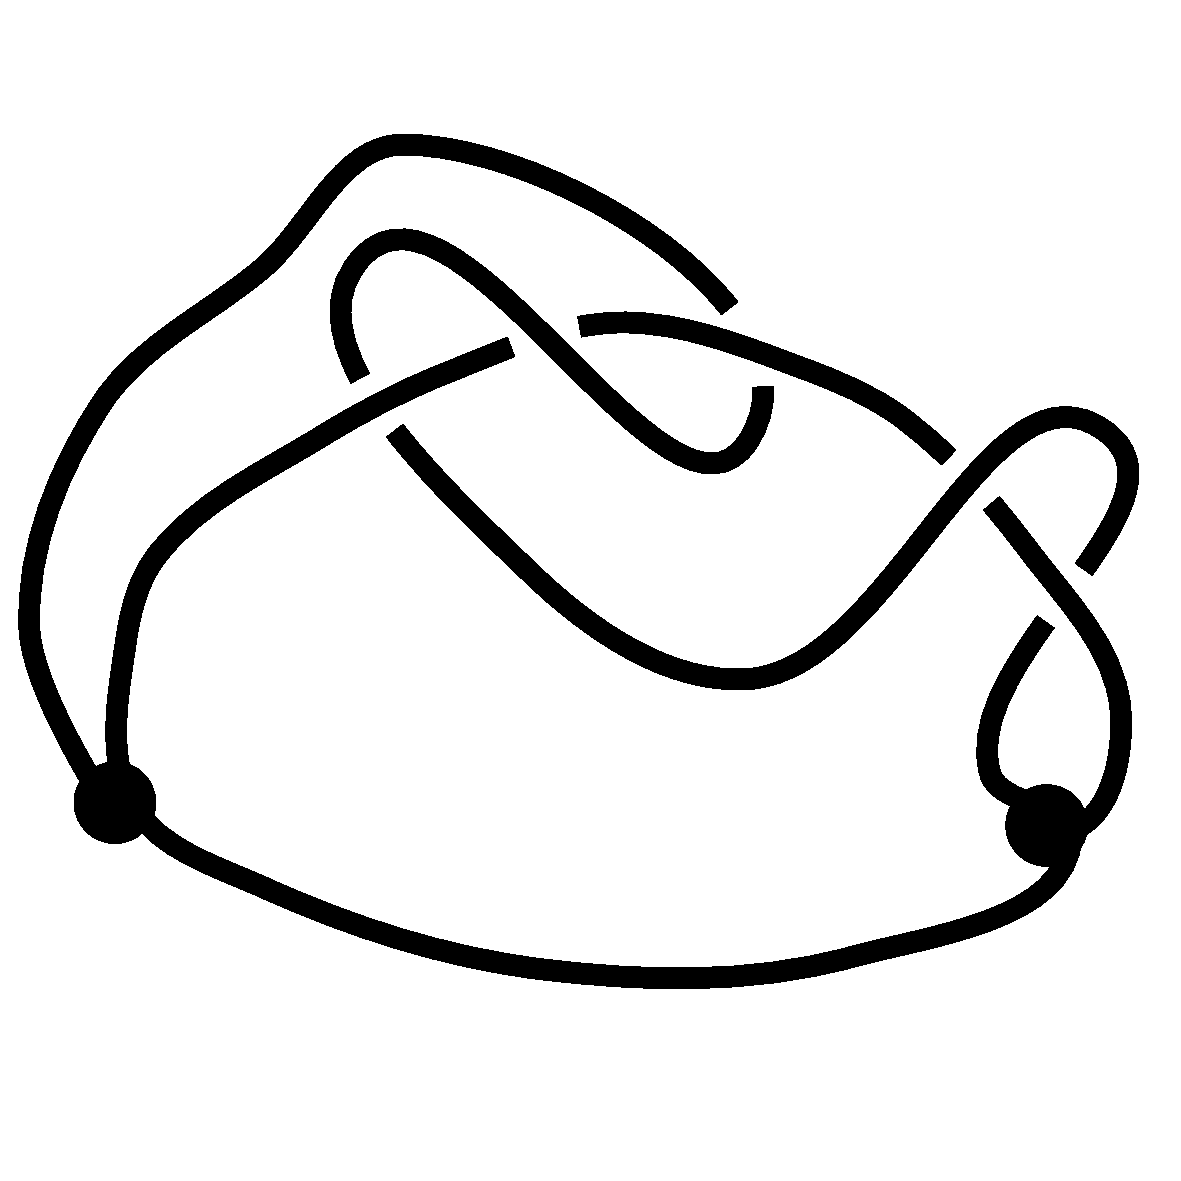
\includegraphics[scale=0.15]{knot_07_03.pdf}
        & \overset{R.II}{\Rightarrow} 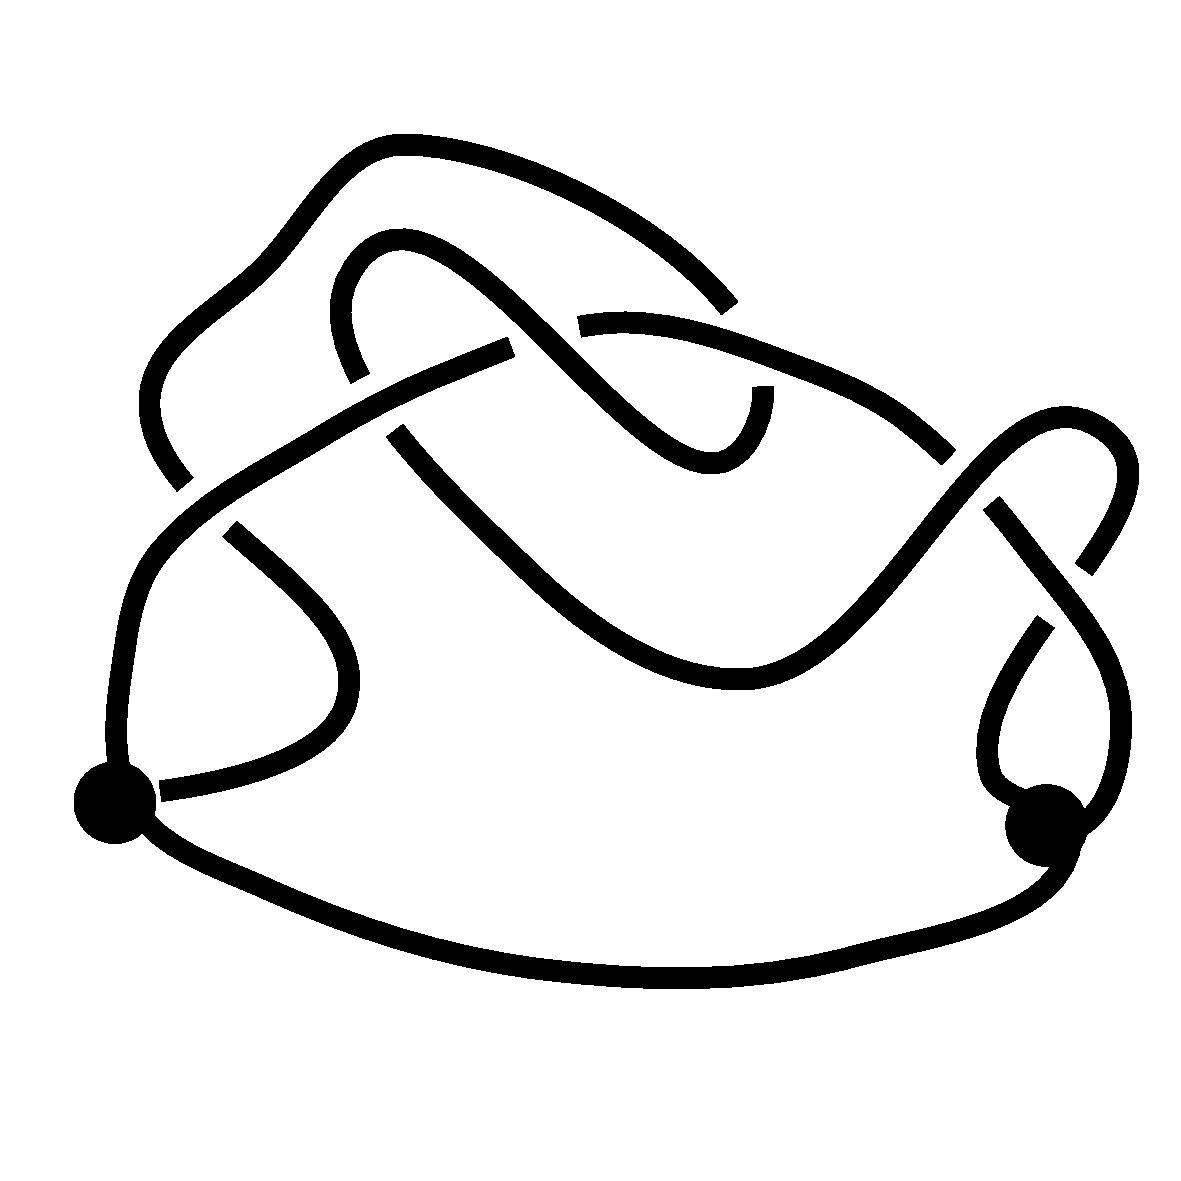
\includegraphics[scale=0.15]{knot_07_04.pdf}\\
        & \overset{R.II}{\Rightarrow} 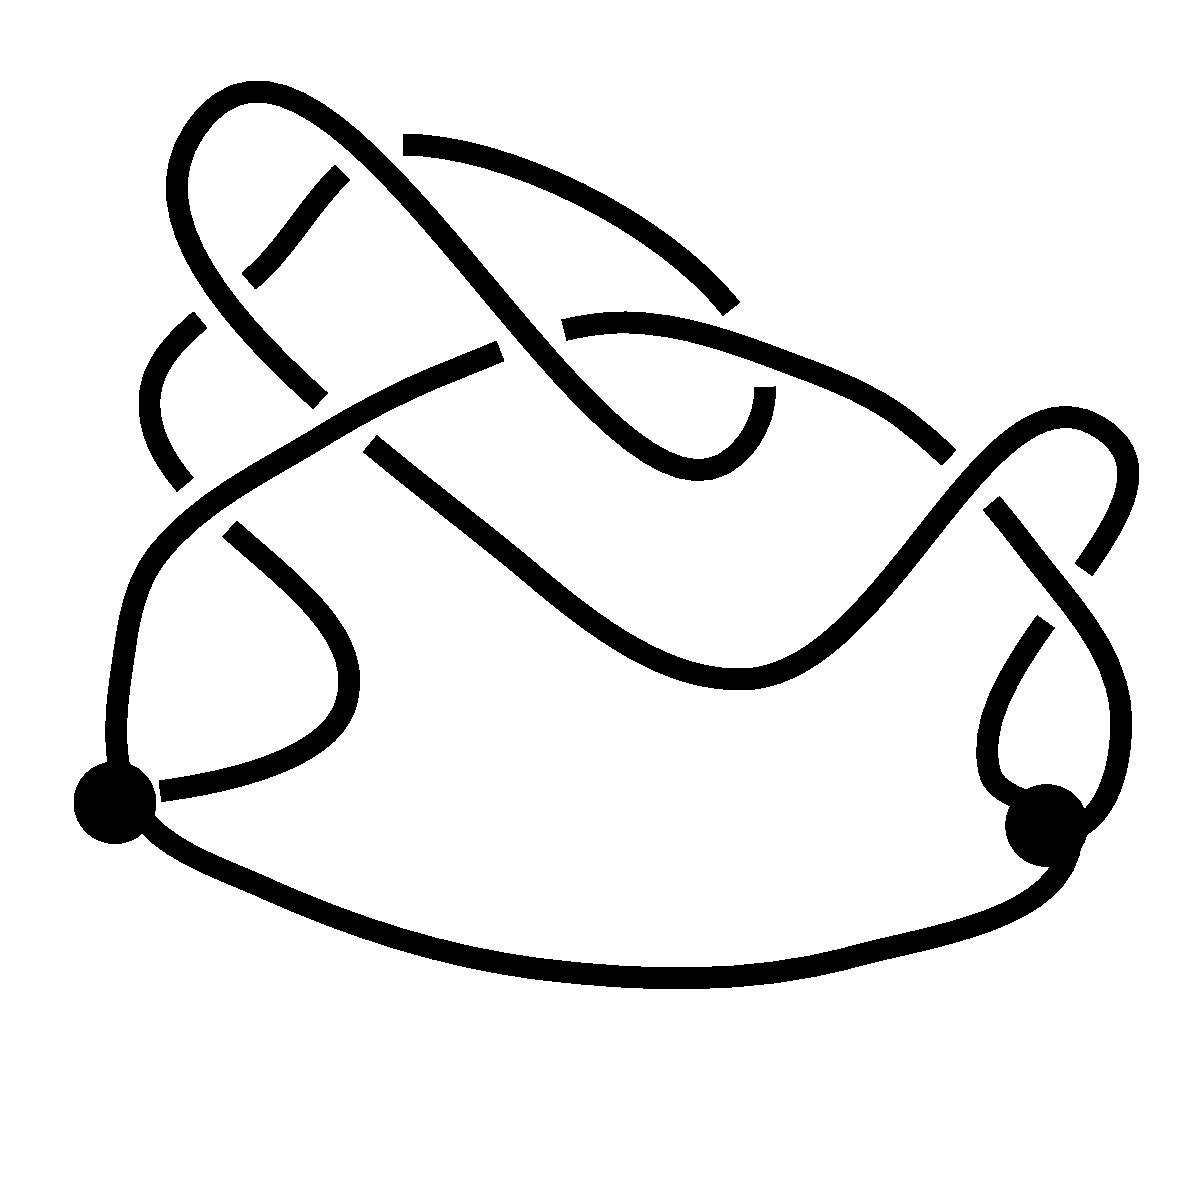
\includegraphics[scale=0.15]{knot_07_05.pdf}
        & \overset{R.III}{\Rightarrow} 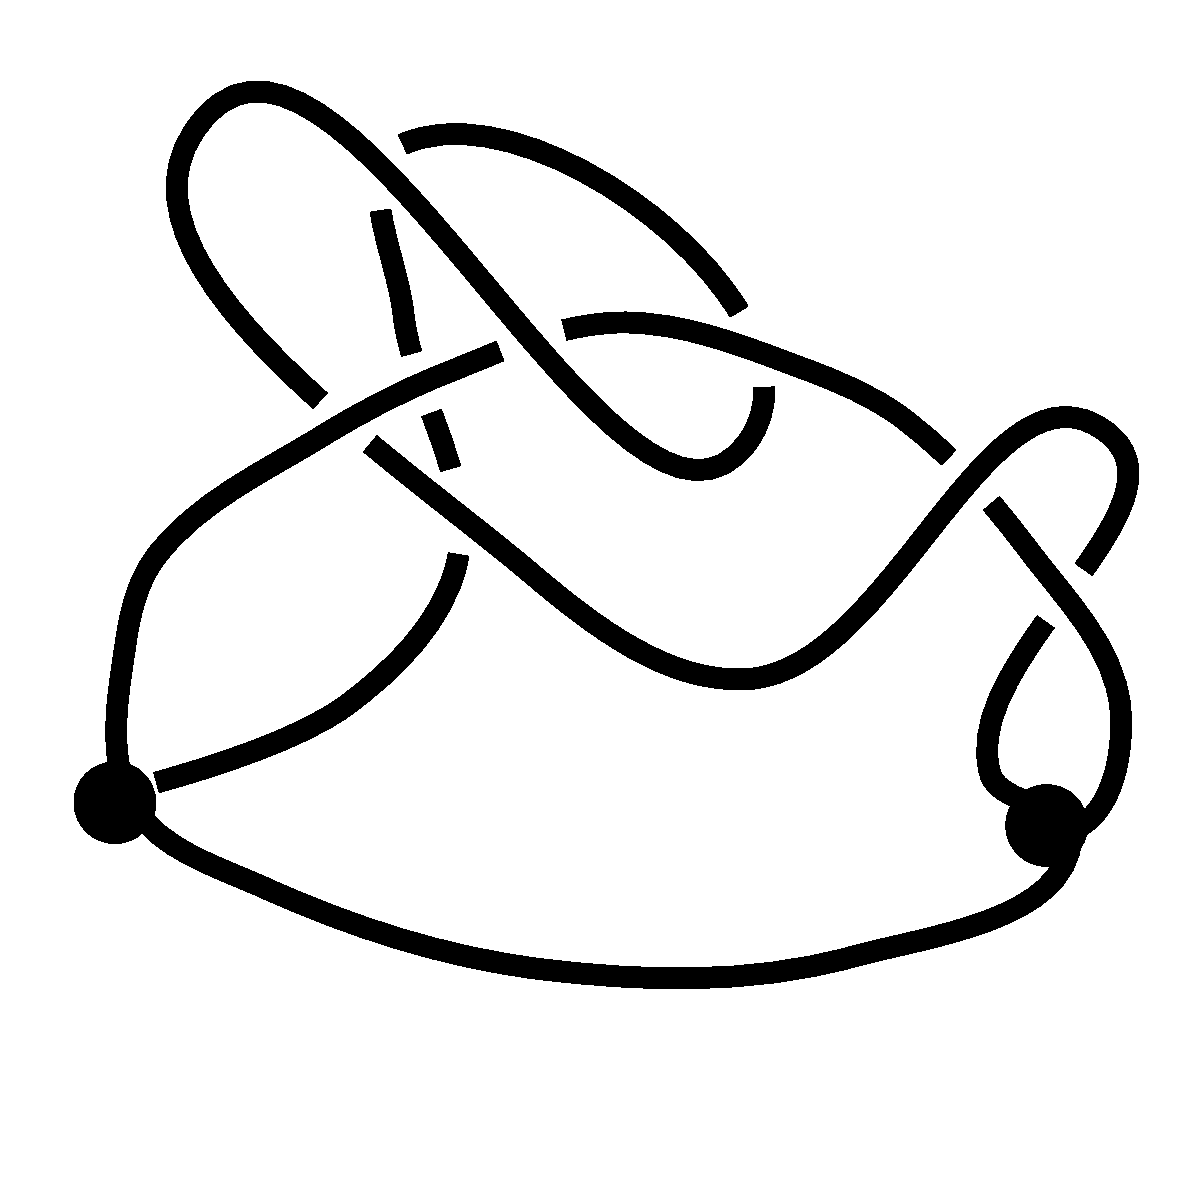
\includegraphics[scale=0.15]{knot_07_06.pdf}
        & \overset{R.III}{\Rightarrow} 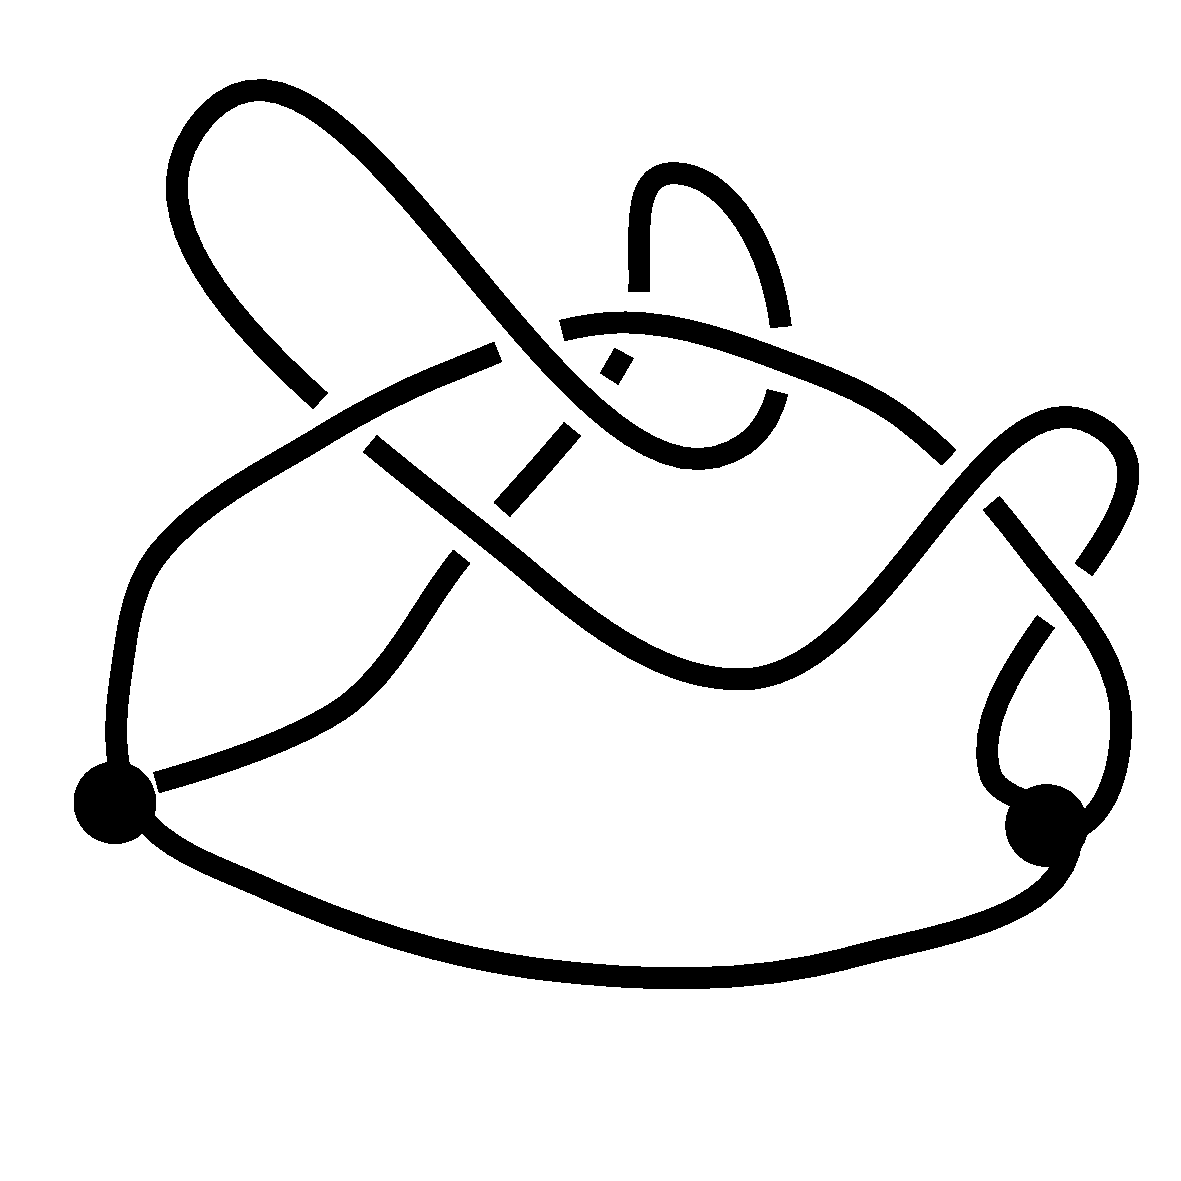
\includegraphics[scale=0.15]{knot_07_07.pdf}\\
        & \overset{R.III}{\Rightarrow} 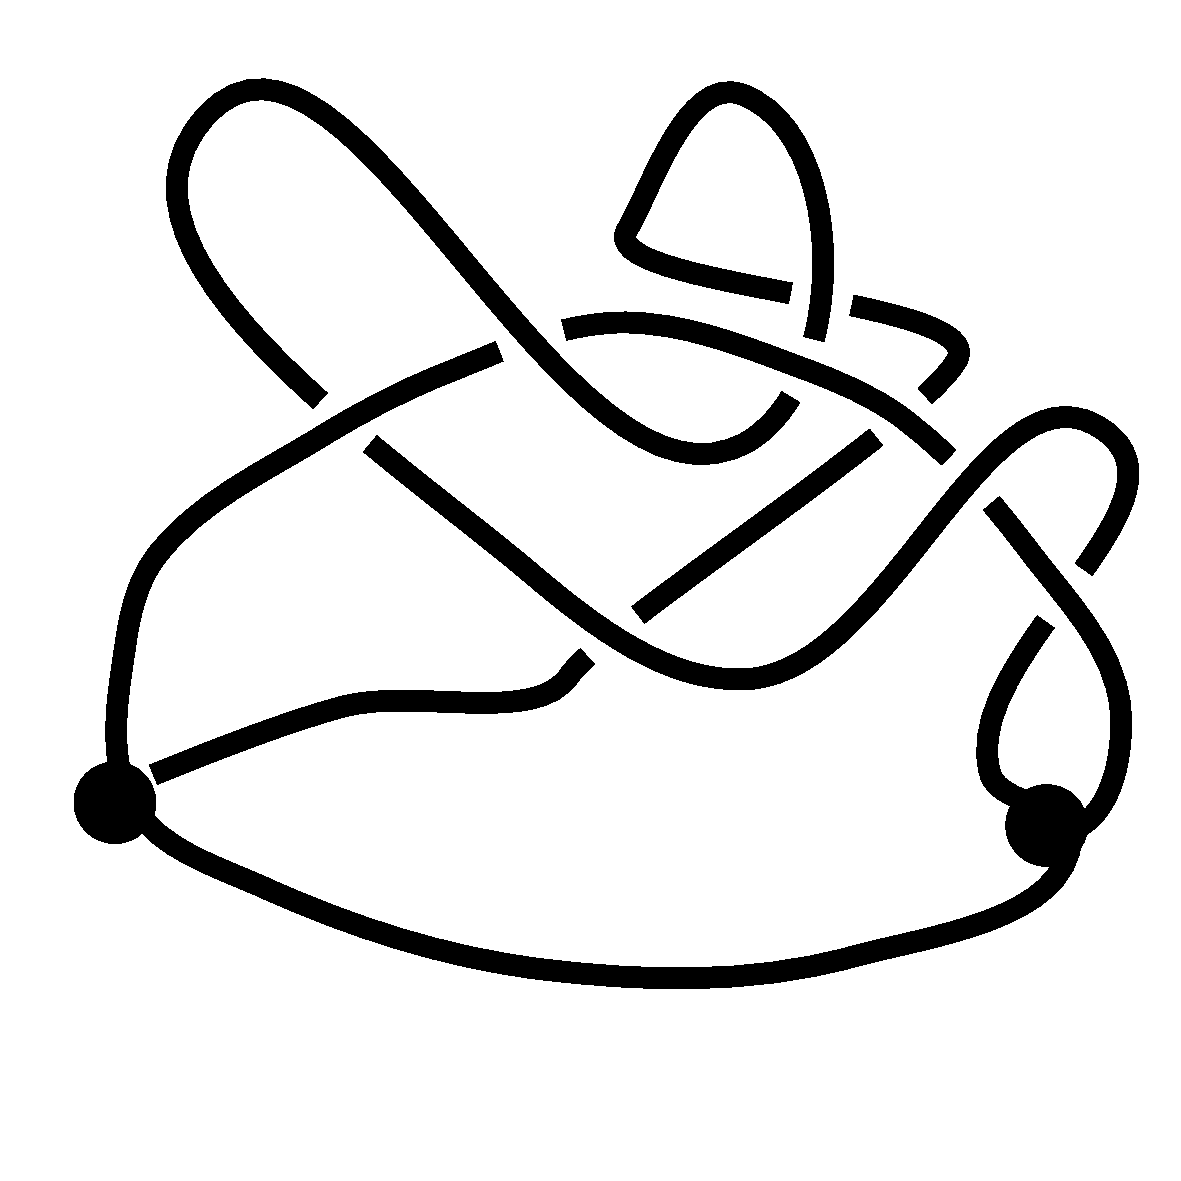
\includegraphics[scale=0.15]{knot_07_08.pdf}
        & \overset{R.I}{\Rightarrow} 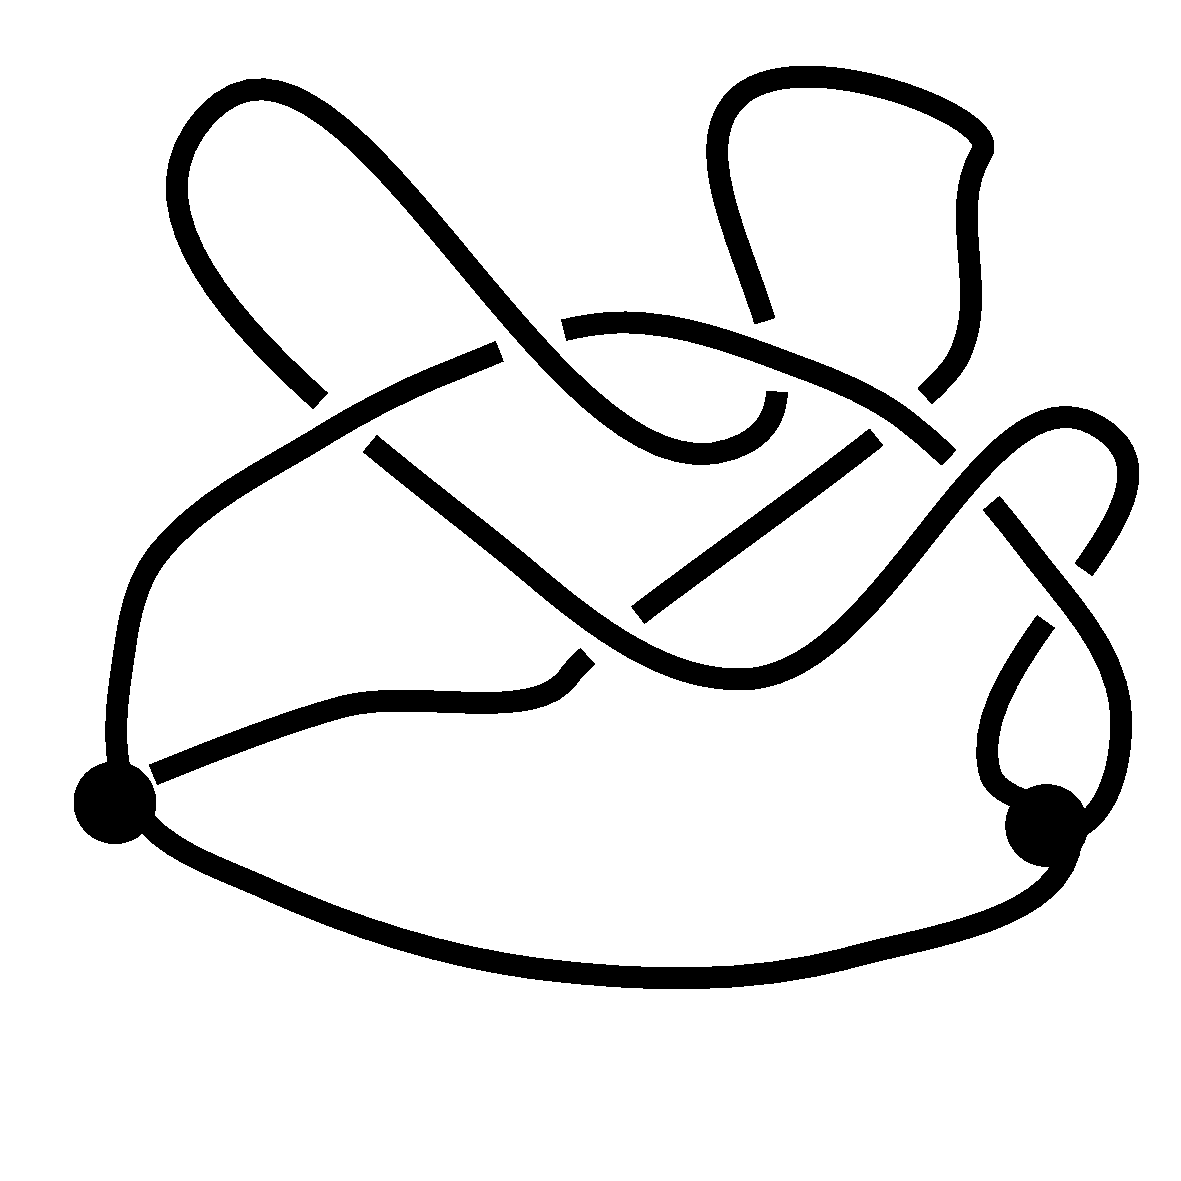
\includegraphics[scale=0.15]{knot_07_09.pdf}
        & \overset{R.II}{\Rightarrow} 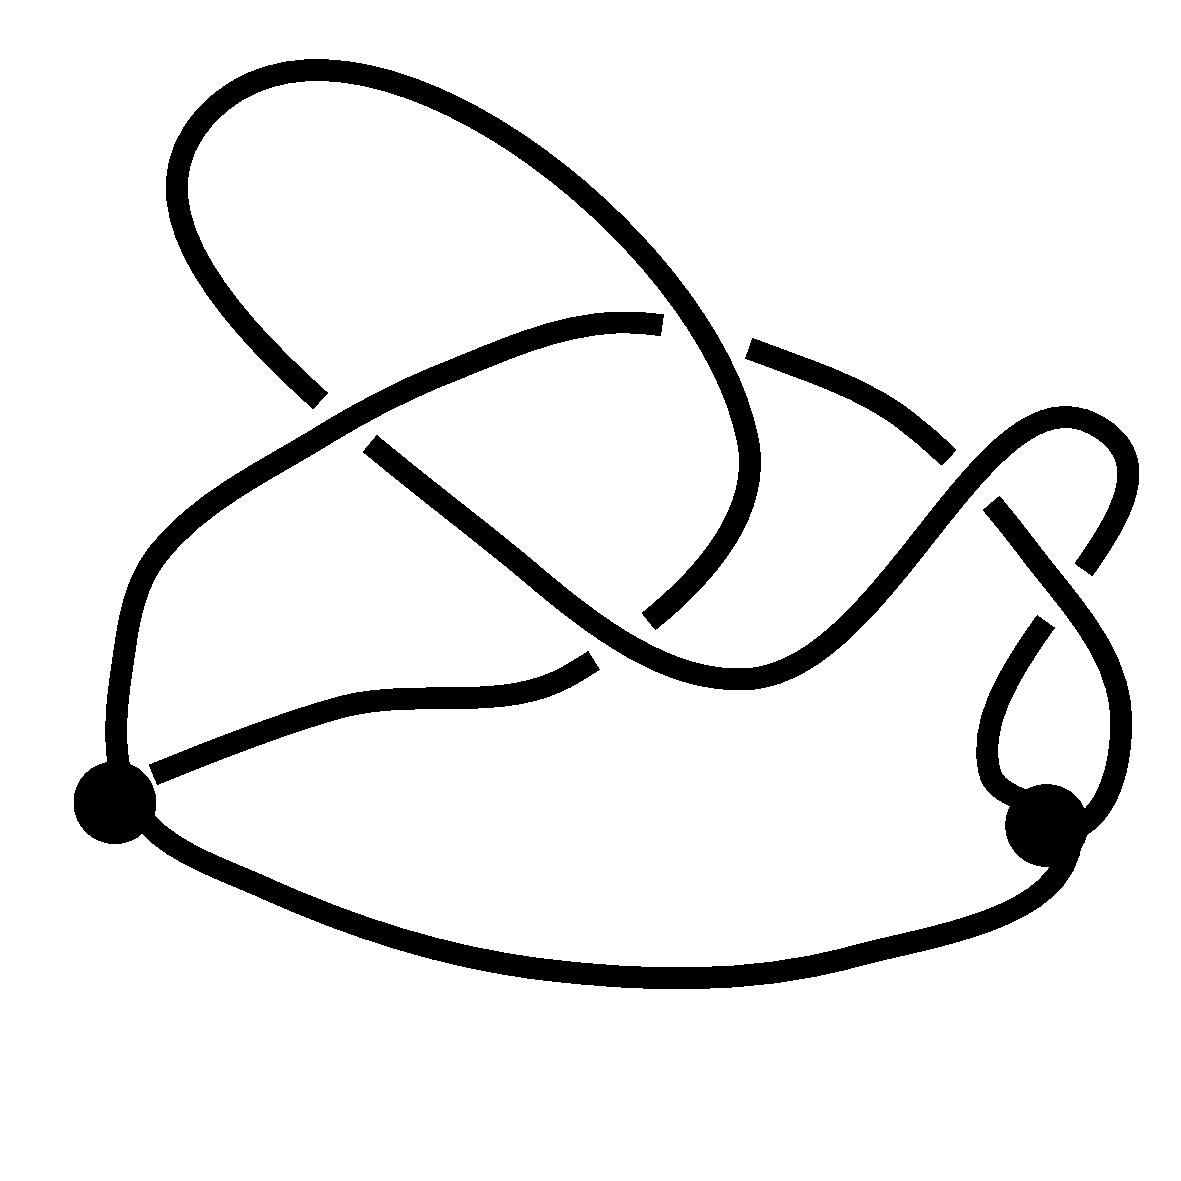
\includegraphics[scale=0.15]{knot_07_10.pdf}\\
        & \overset{R.II}{\Rightarrow} 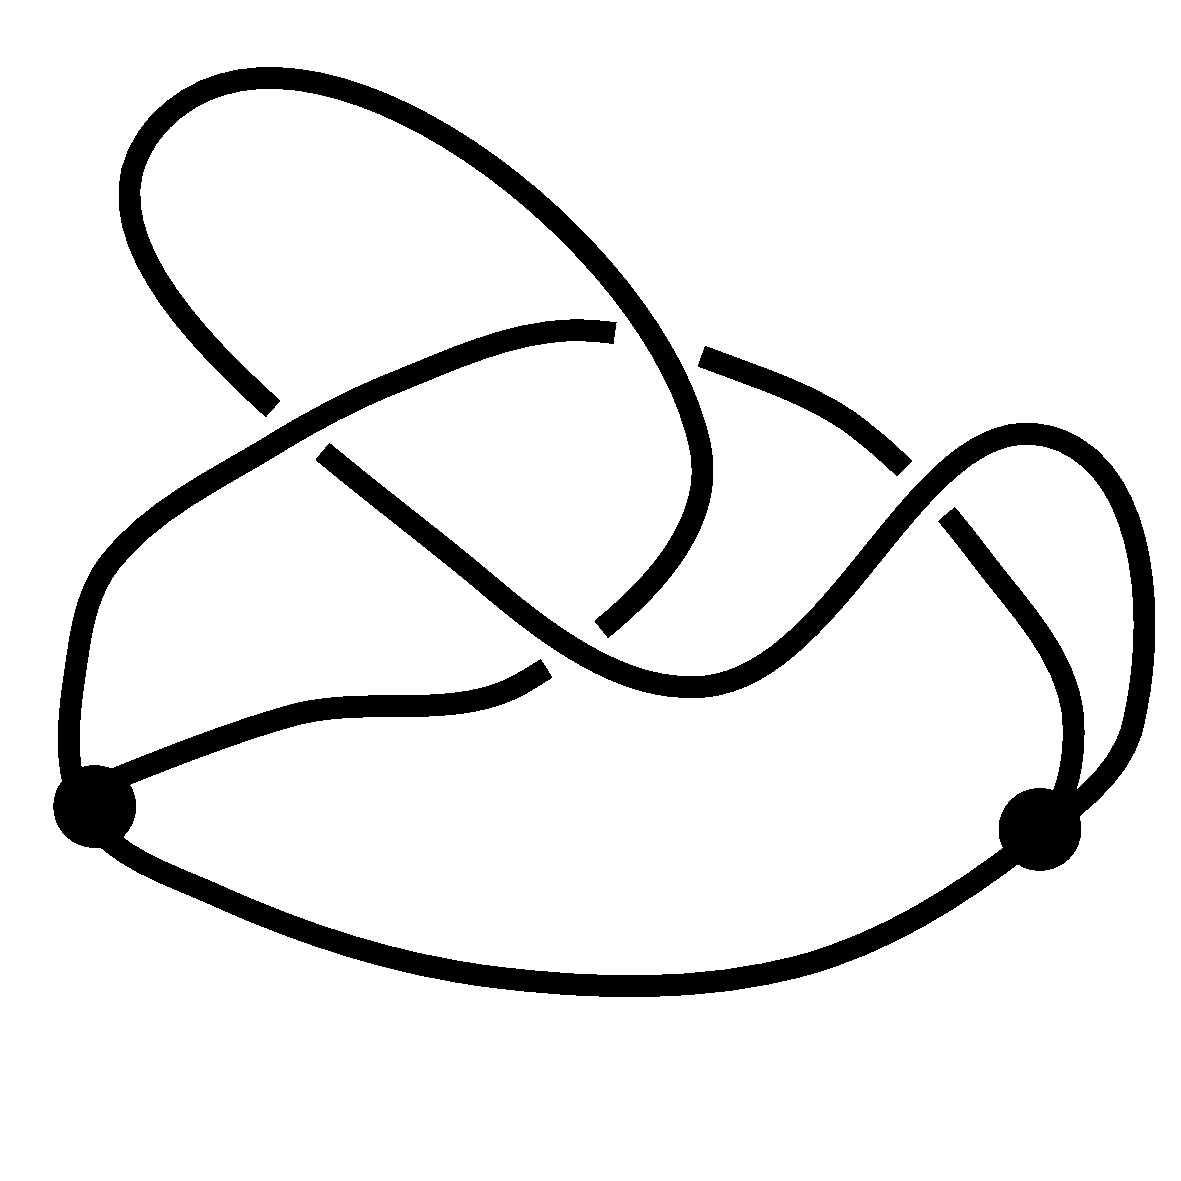
\includegraphics[scale=0.15]{knot_07_11.pdf}
        & \overset{R.II}{\Rightarrow} 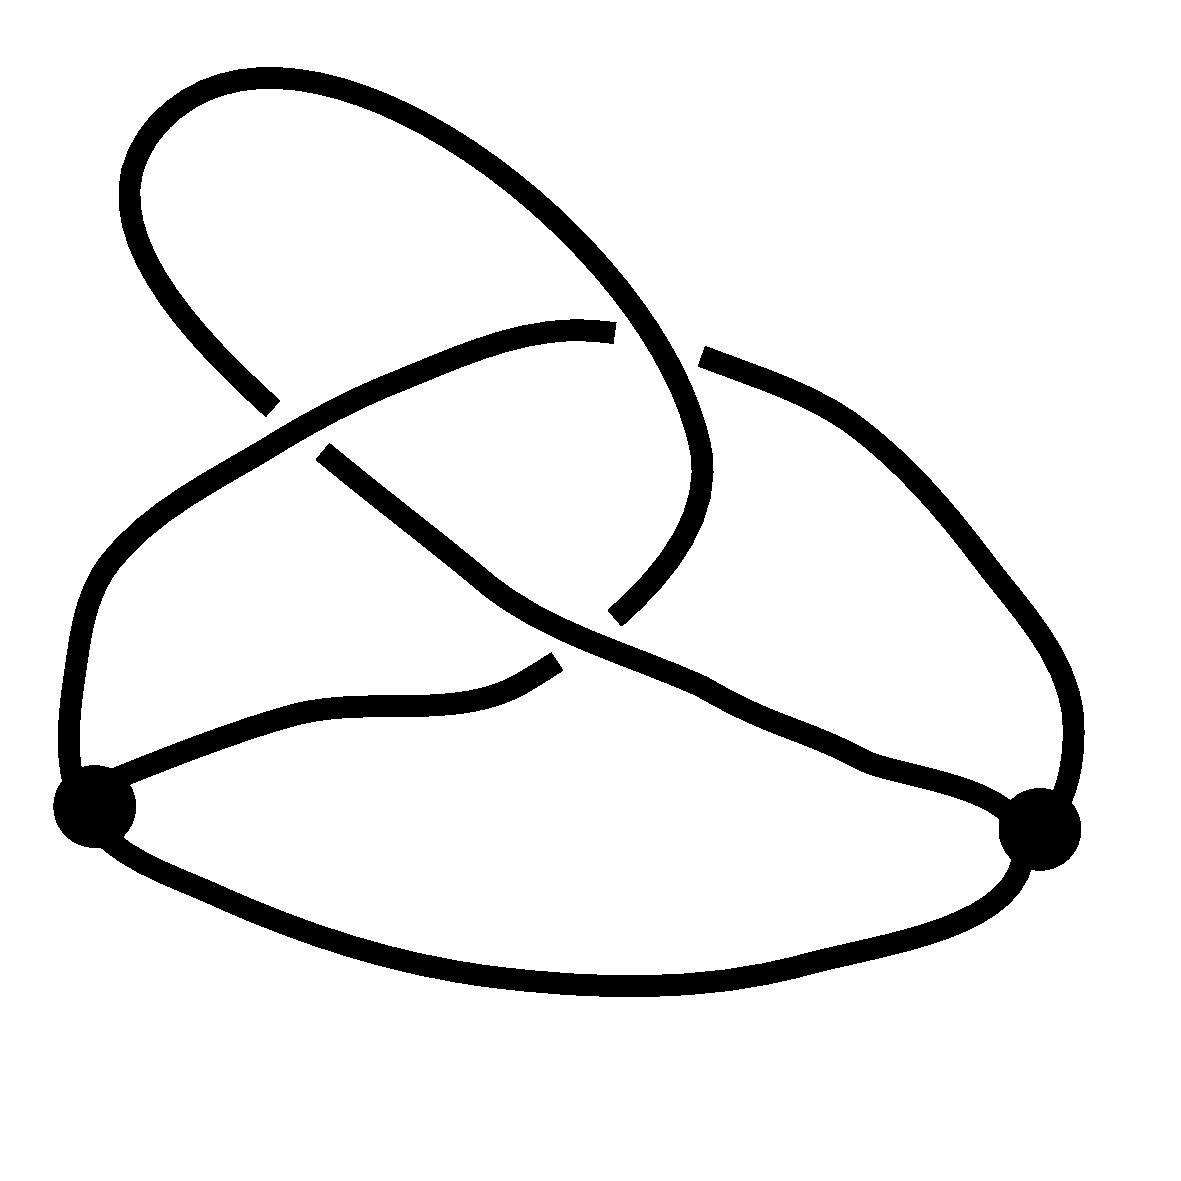
\includegraphics[scale=0.15]{knot_07_12.pdf}
        & \overset{}{\Rightarrow} \tilde{g}(G)
       \end{align}


      \hrulefill


 \item
      $f(G),g(G)$は、それぞれ$\tilde{f}(G),\tilde{g}(G)$で表された
      空間グラフとする。
      このとき、
      以下の設問に答えよ。
      \begin{equation}
       \begin{matrix}
        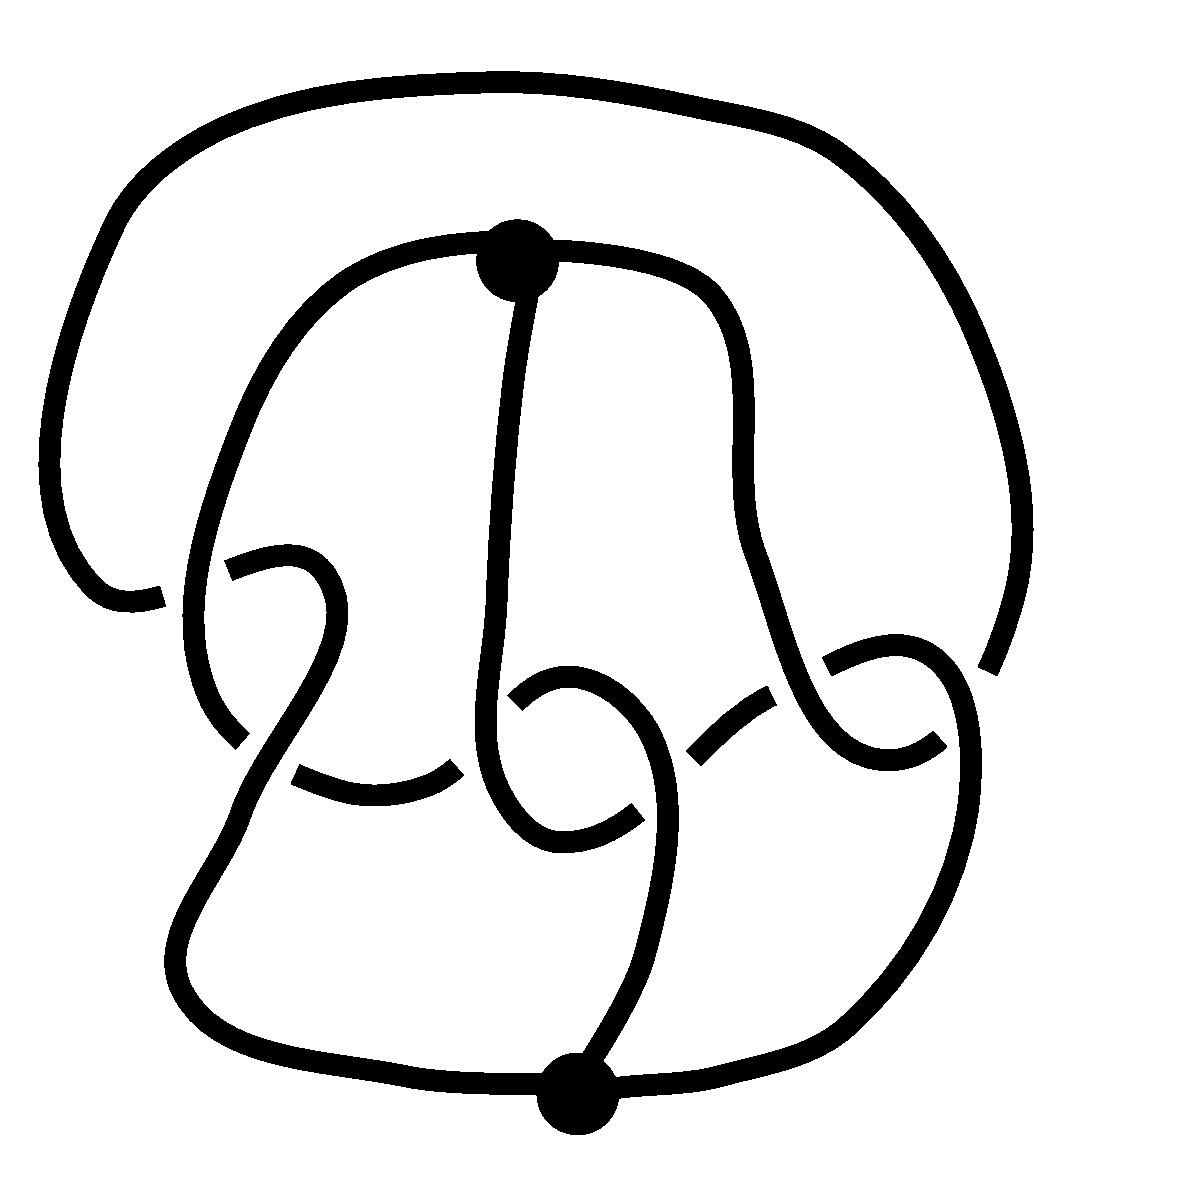
\includegraphics[scale=0.2]{knot_08_01.pdf} &
       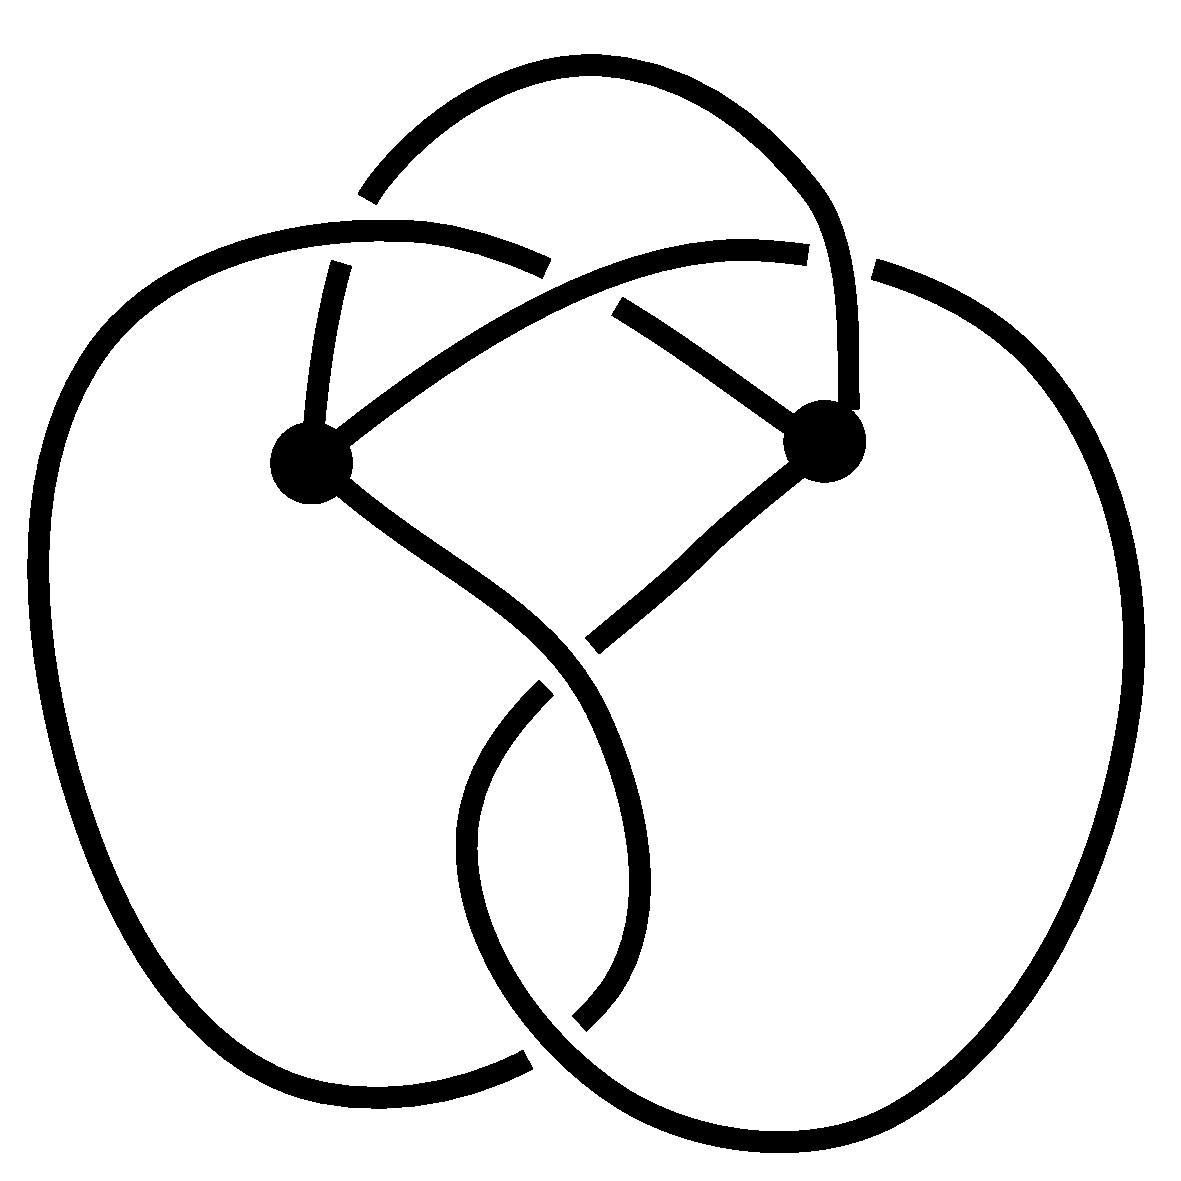
\includegraphics[scale=0.2]{knot_08_99.pdf}\\
       \tilde{f}(G) & \tilde{g}(G)
       \end{matrix}
       \end{equation}
      
      \begin{enumerate}
       \item
            $f(G)$と$g(G)$は同型であることを
            $\mathbb{R}^{3}$内の直接の変形で確かめよ。

            \dotfill

            \begin{align}
             \tilde{f}(G)
             & \Rightarrow 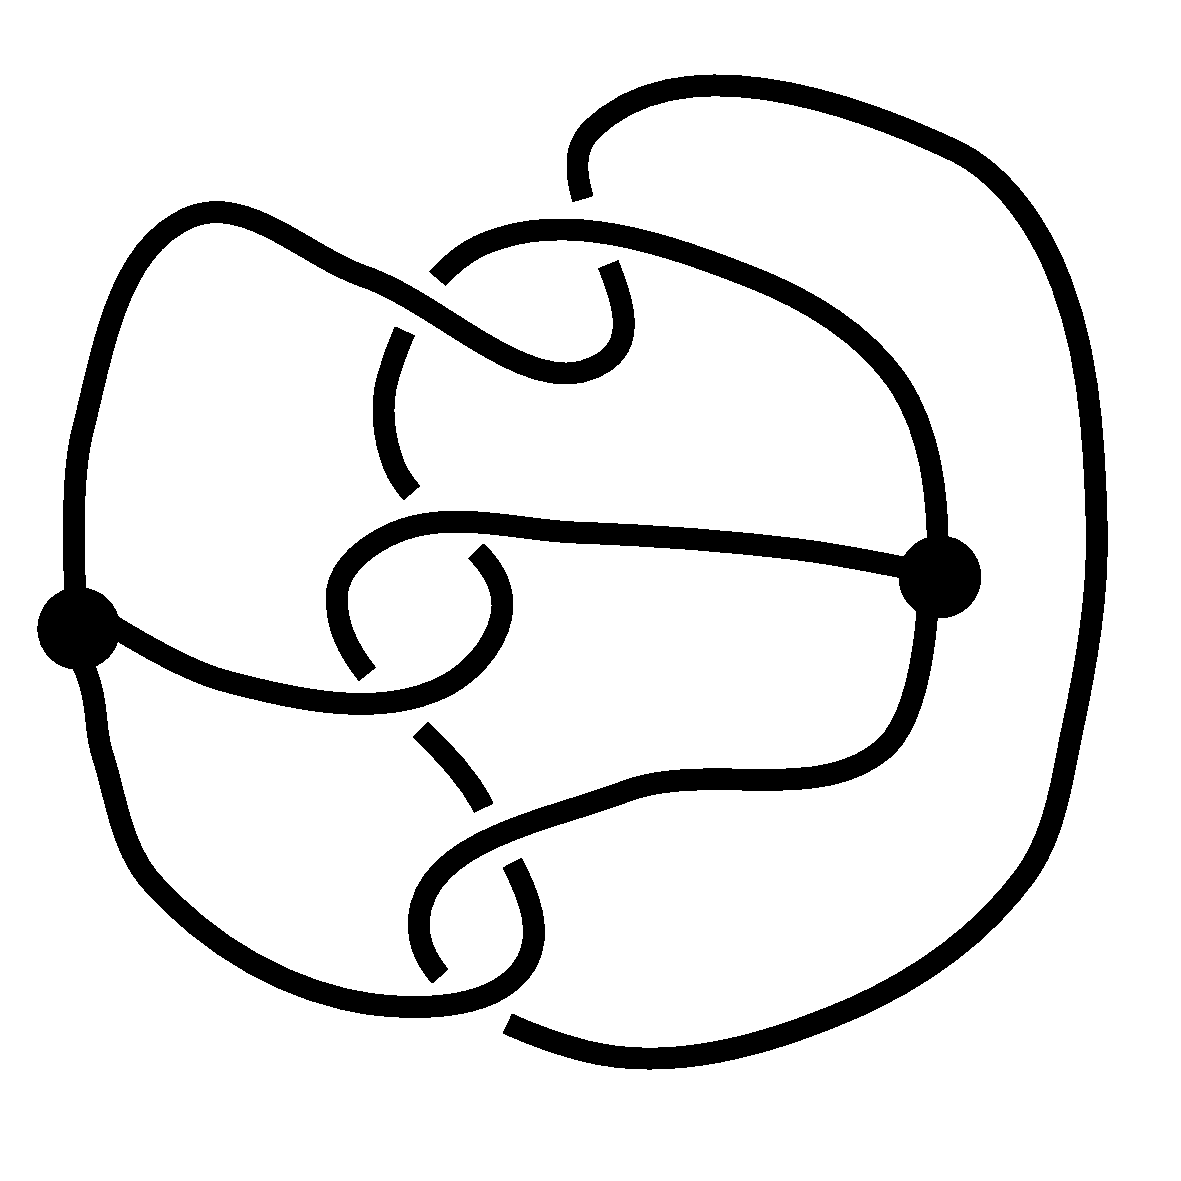
\includegraphics[scale=0.15]{knot_08_a02.pdf}
             & \Rightarrow 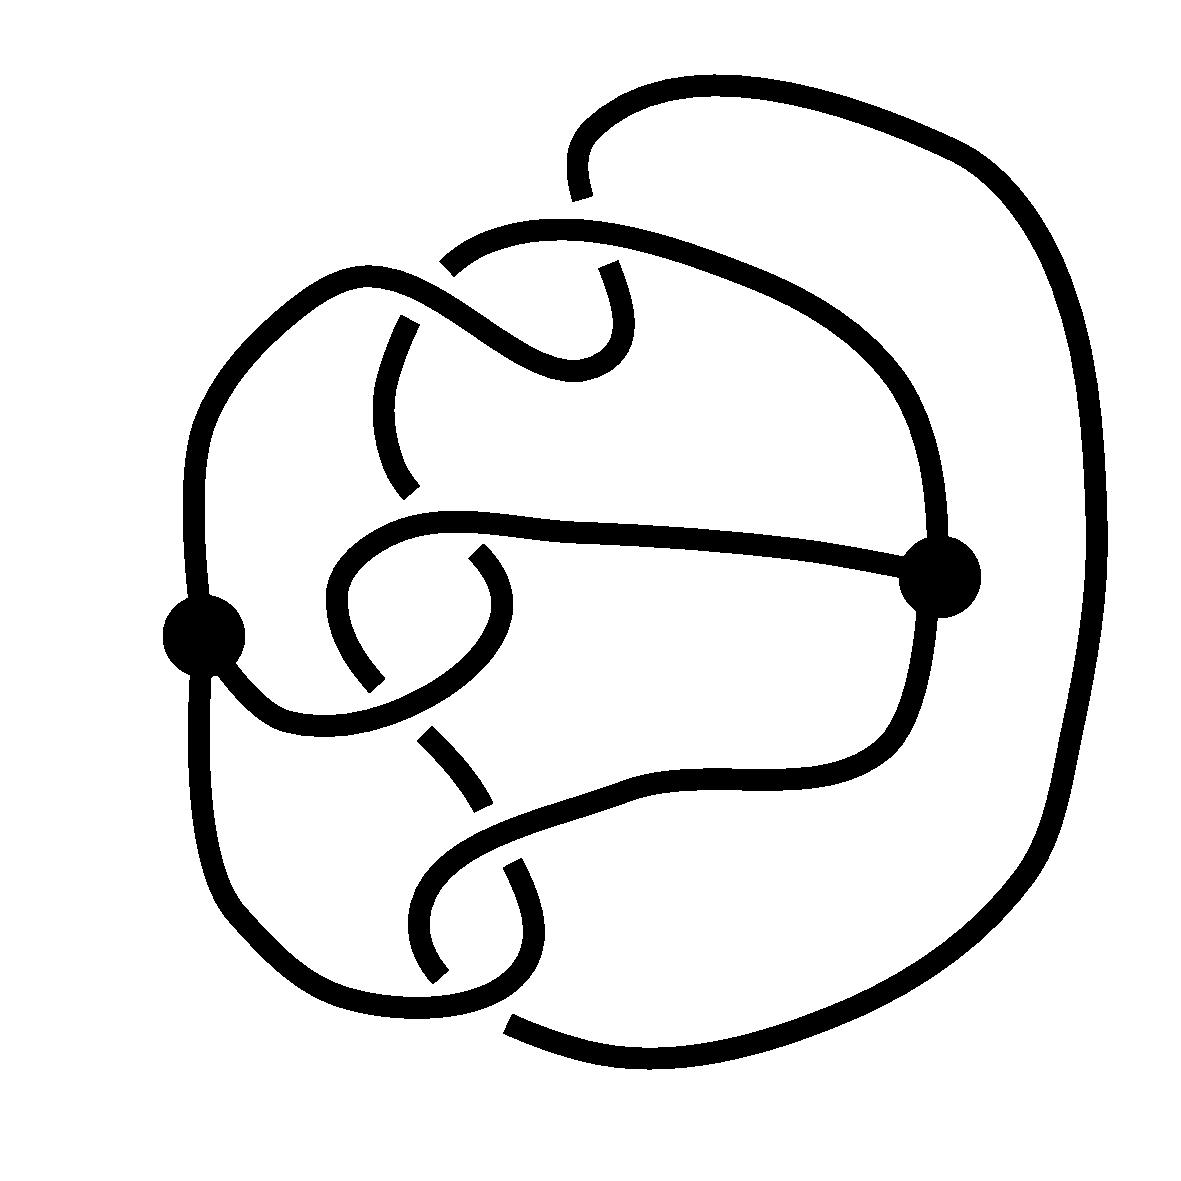
\includegraphics[scale=0.15]{knot_08_a03.pdf}
             & \Rightarrow 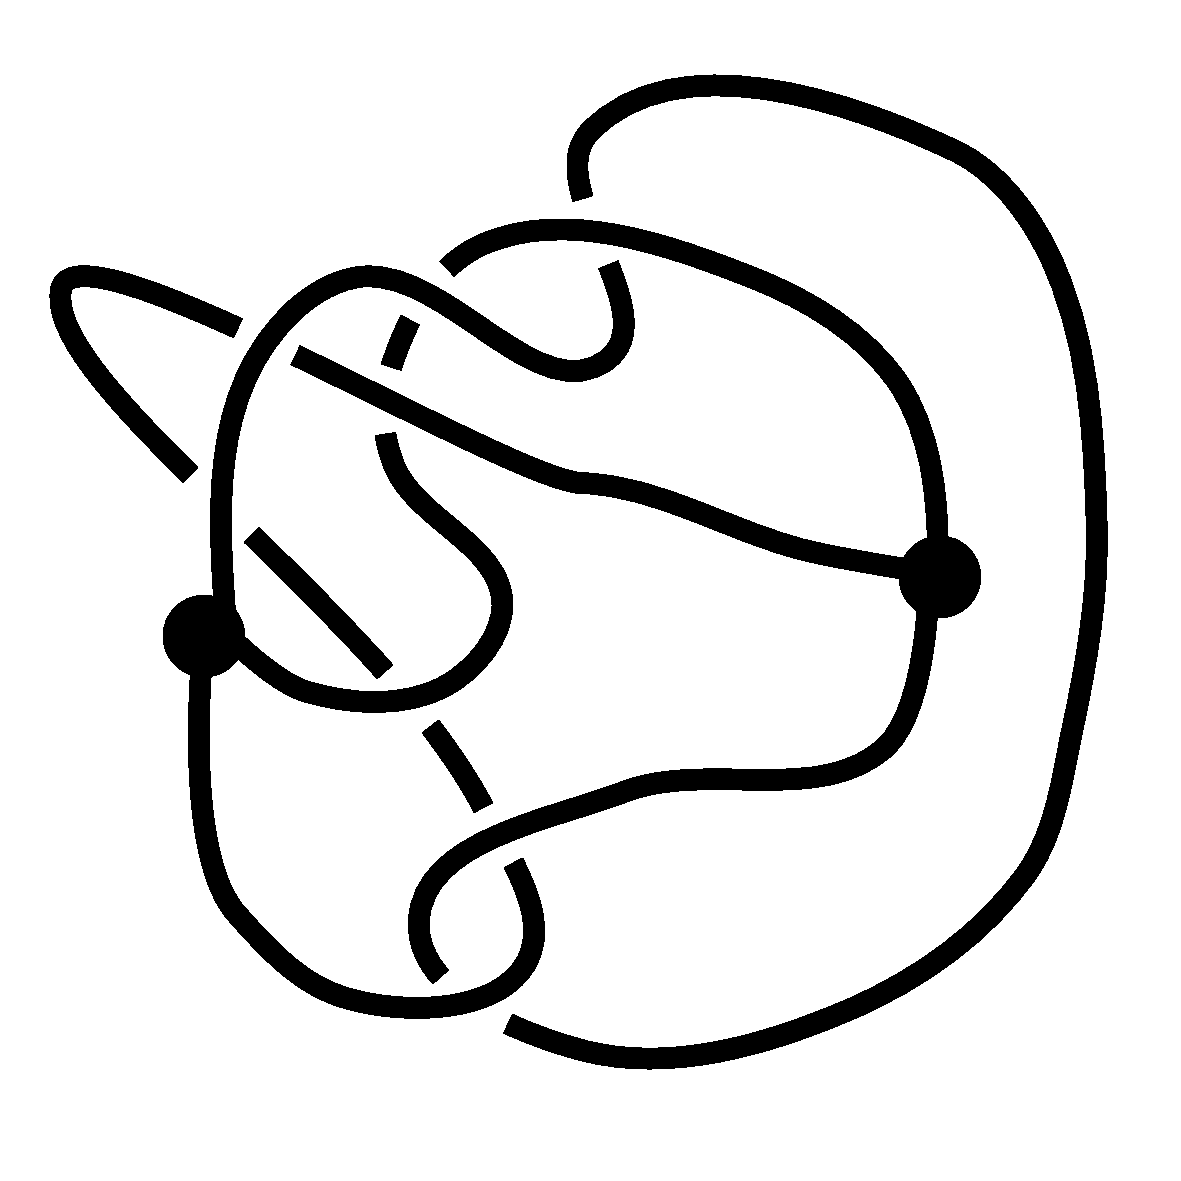
\includegraphics[scale=0.15]{knot_08_a04.pdf}\\
             & \Rightarrow 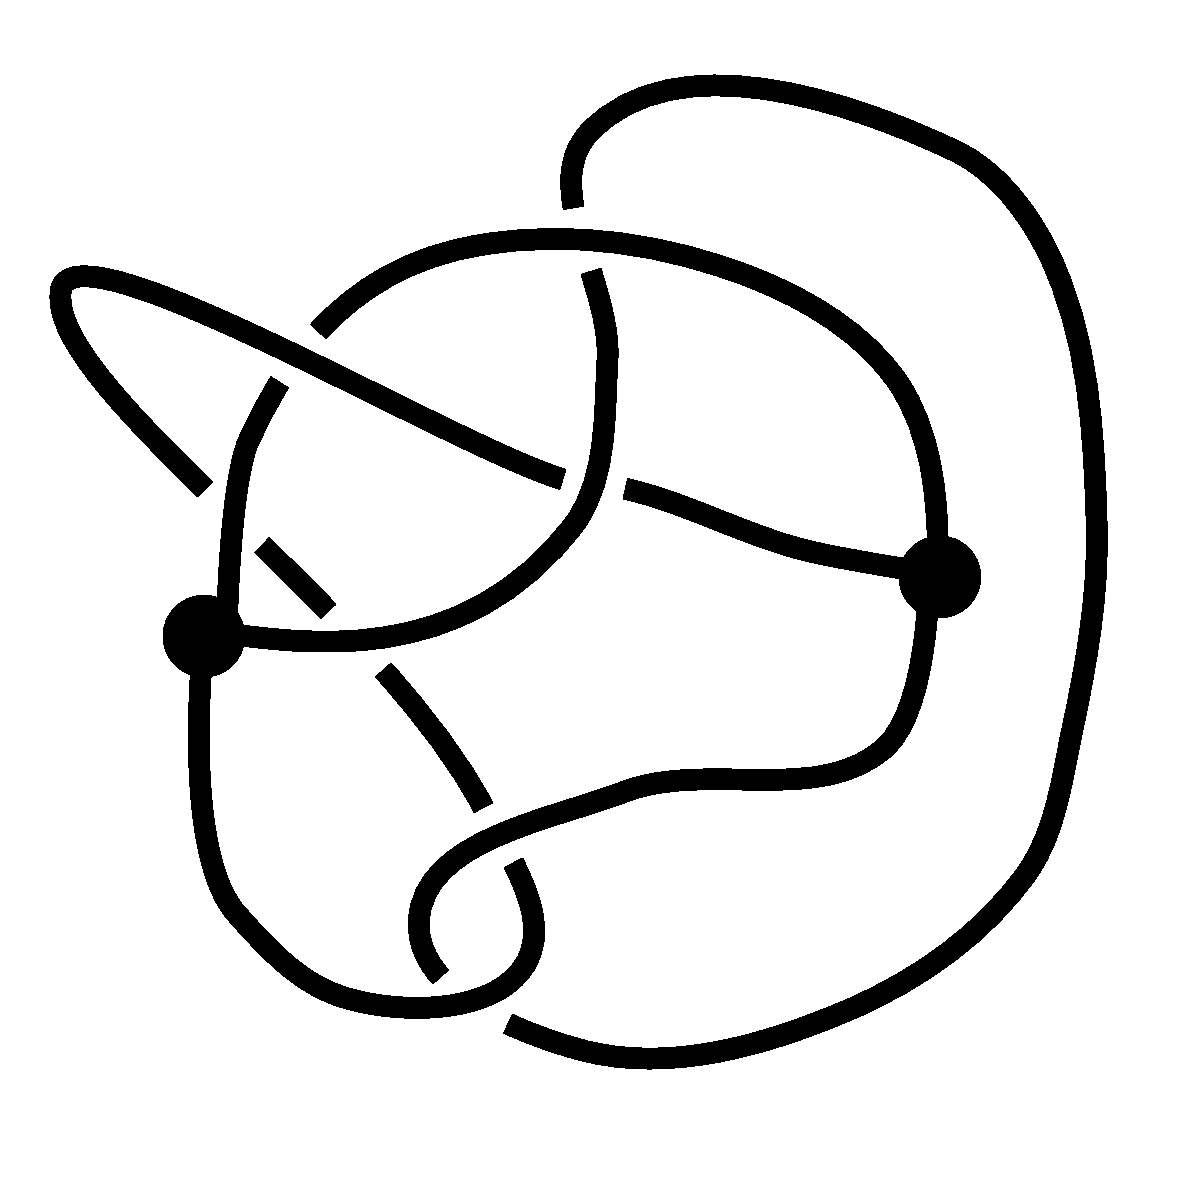
\includegraphics[scale=0.15]{knot_08_a05.pdf}
             & \Rightarrow 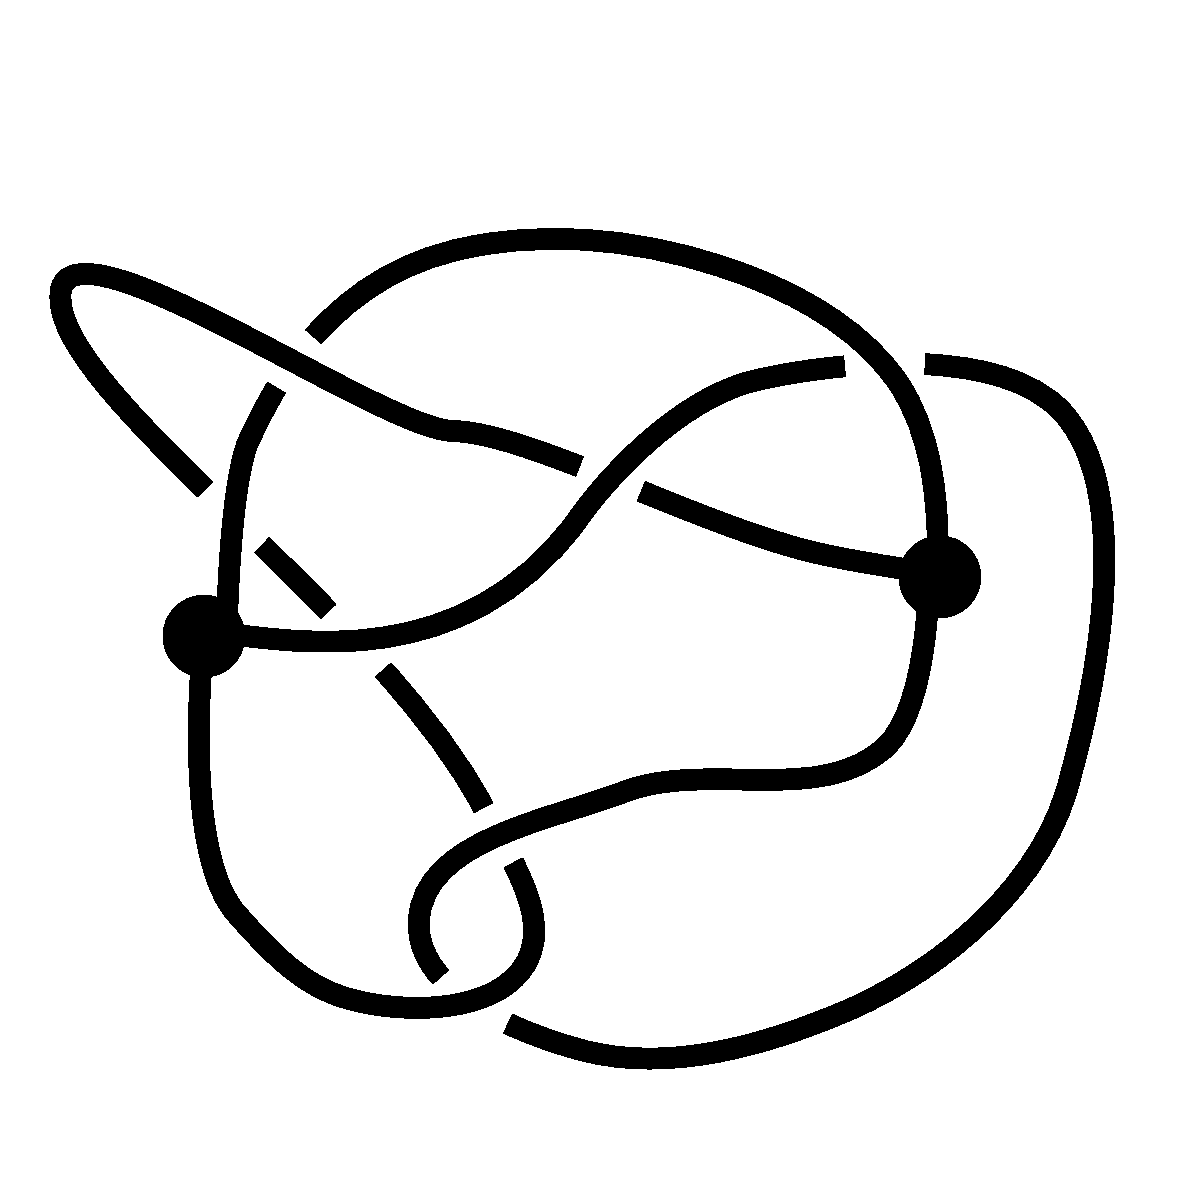
\includegraphics[scale=0.15]{knot_08_a06.pdf}
             & \Rightarrow 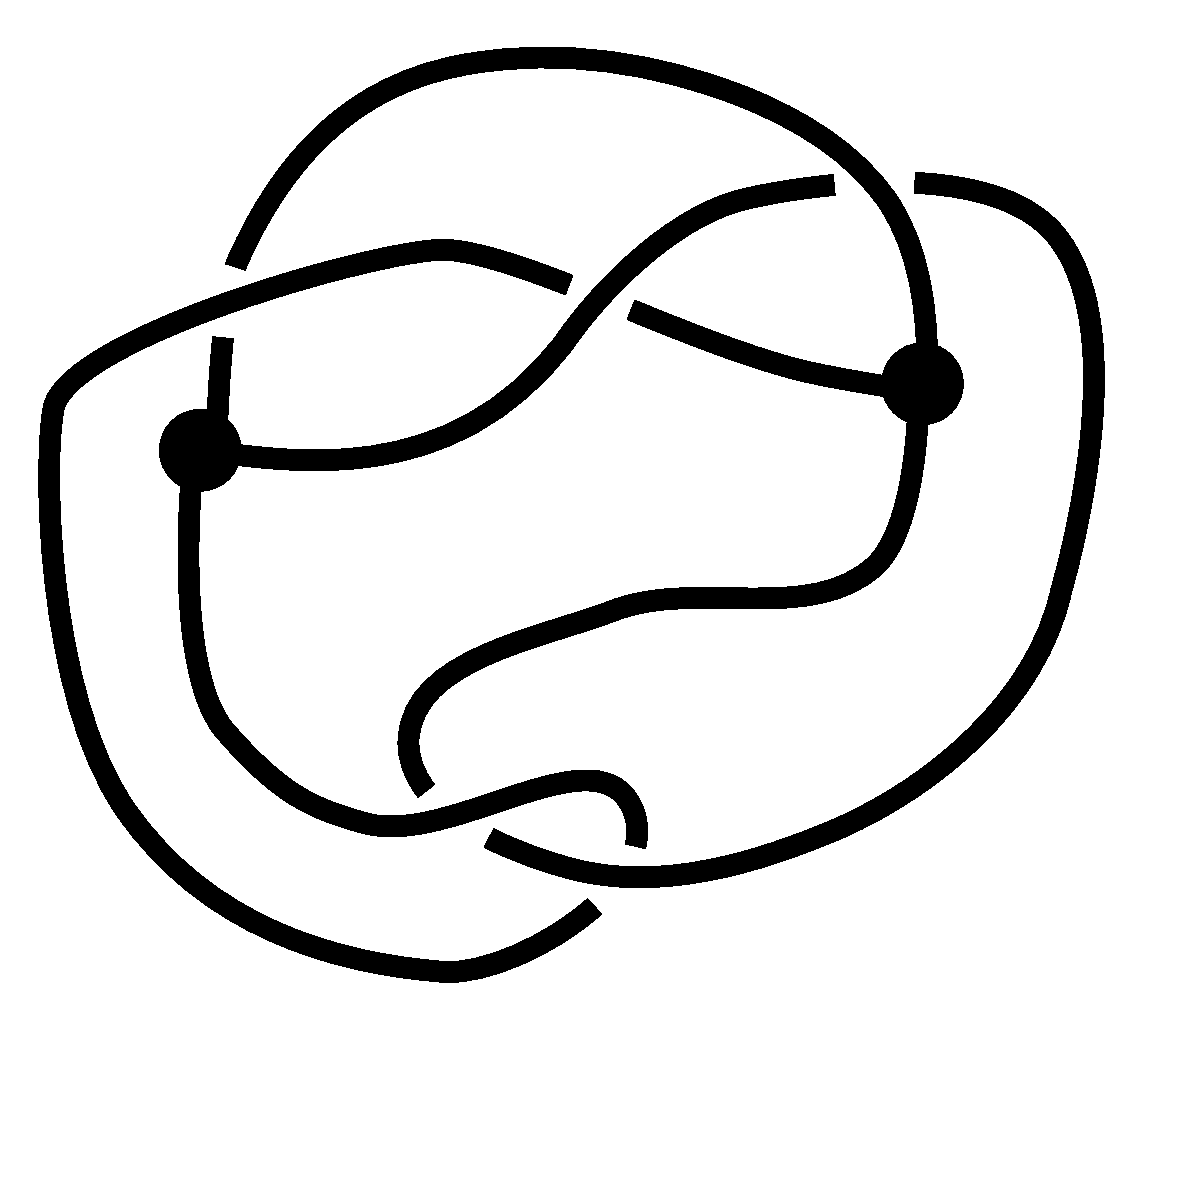
\includegraphics[scale=0.15]{knot_08_a07.pdf}\\
             & \Rightarrow 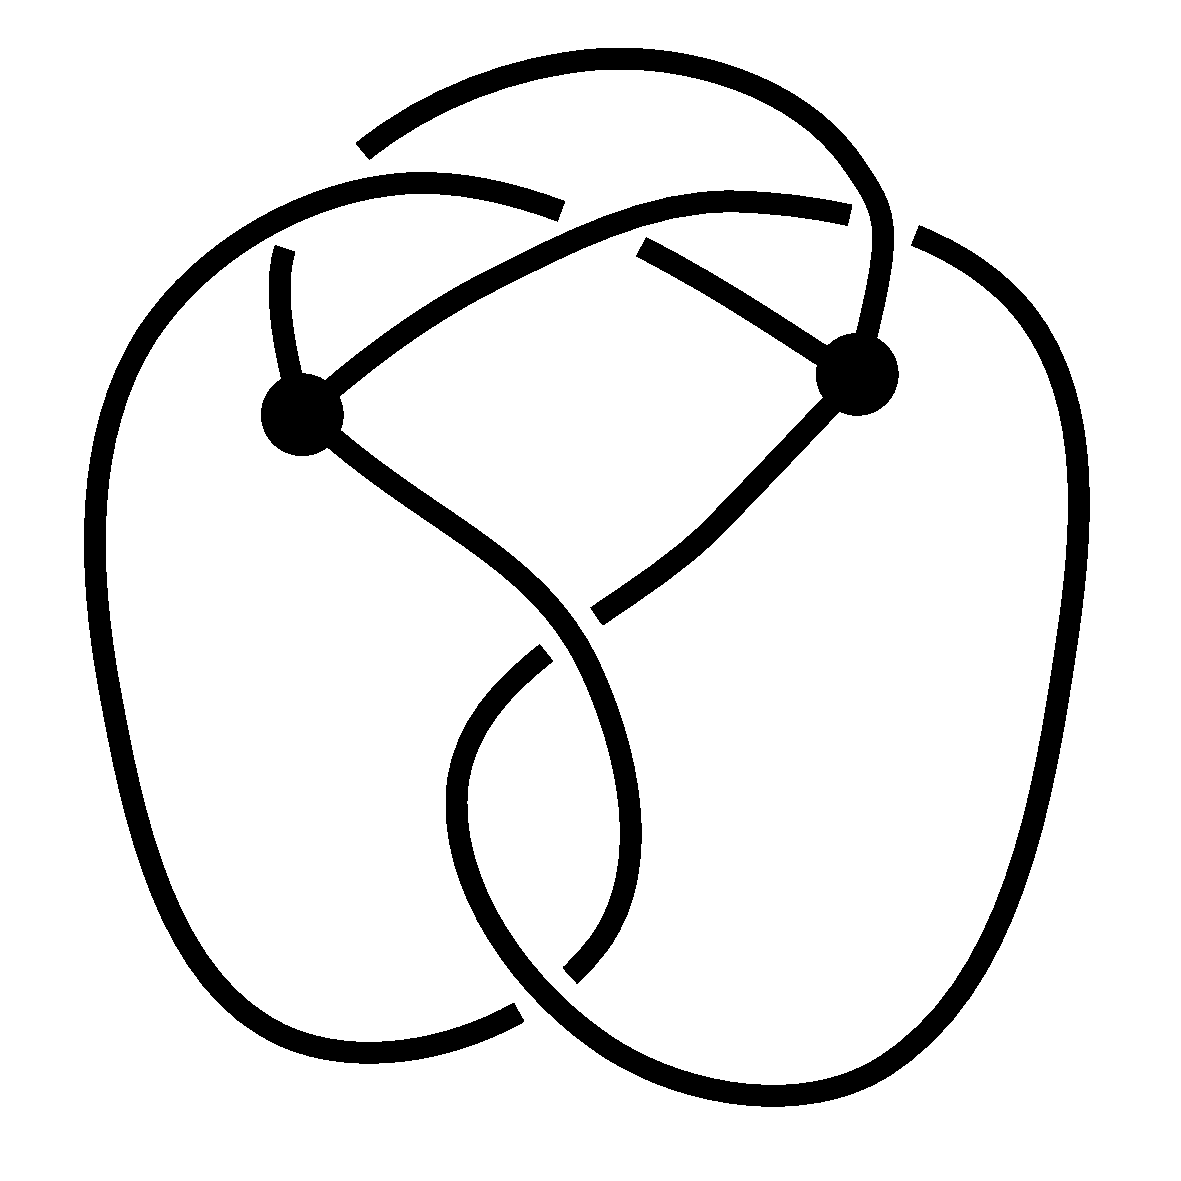
\includegraphics[scale=0.15]{knot_08_a08.pdf}
             & \overset{}{\Rightarrow} \tilde{g}(G)
            \end{align}

            \hrulefill

       \item
            $\tilde{f}(G)$と$\tilde{g}(G)$の間の
            Reidemeister 変形の列を具体的に図示せよ。

            \dotfill

            \begin{align}
             &\tilde{f}(G)
             & \overset{}{\Rightarrow} 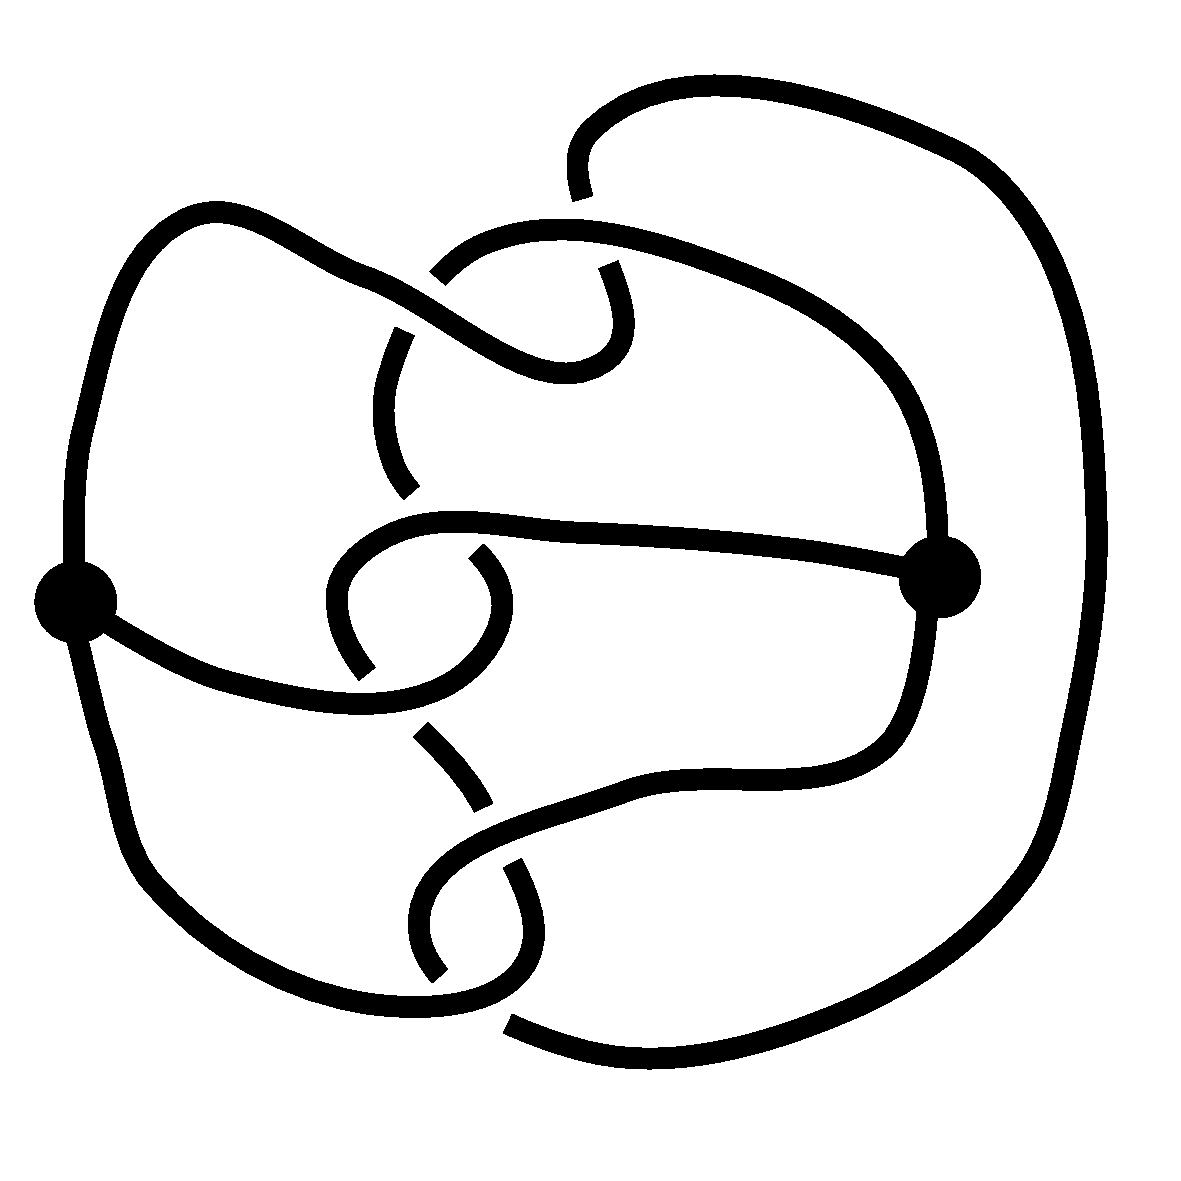
\includegraphics[scale=0.15]{knot_08_b02.pdf}
             & \overset{R.II}{\Rightarrow} 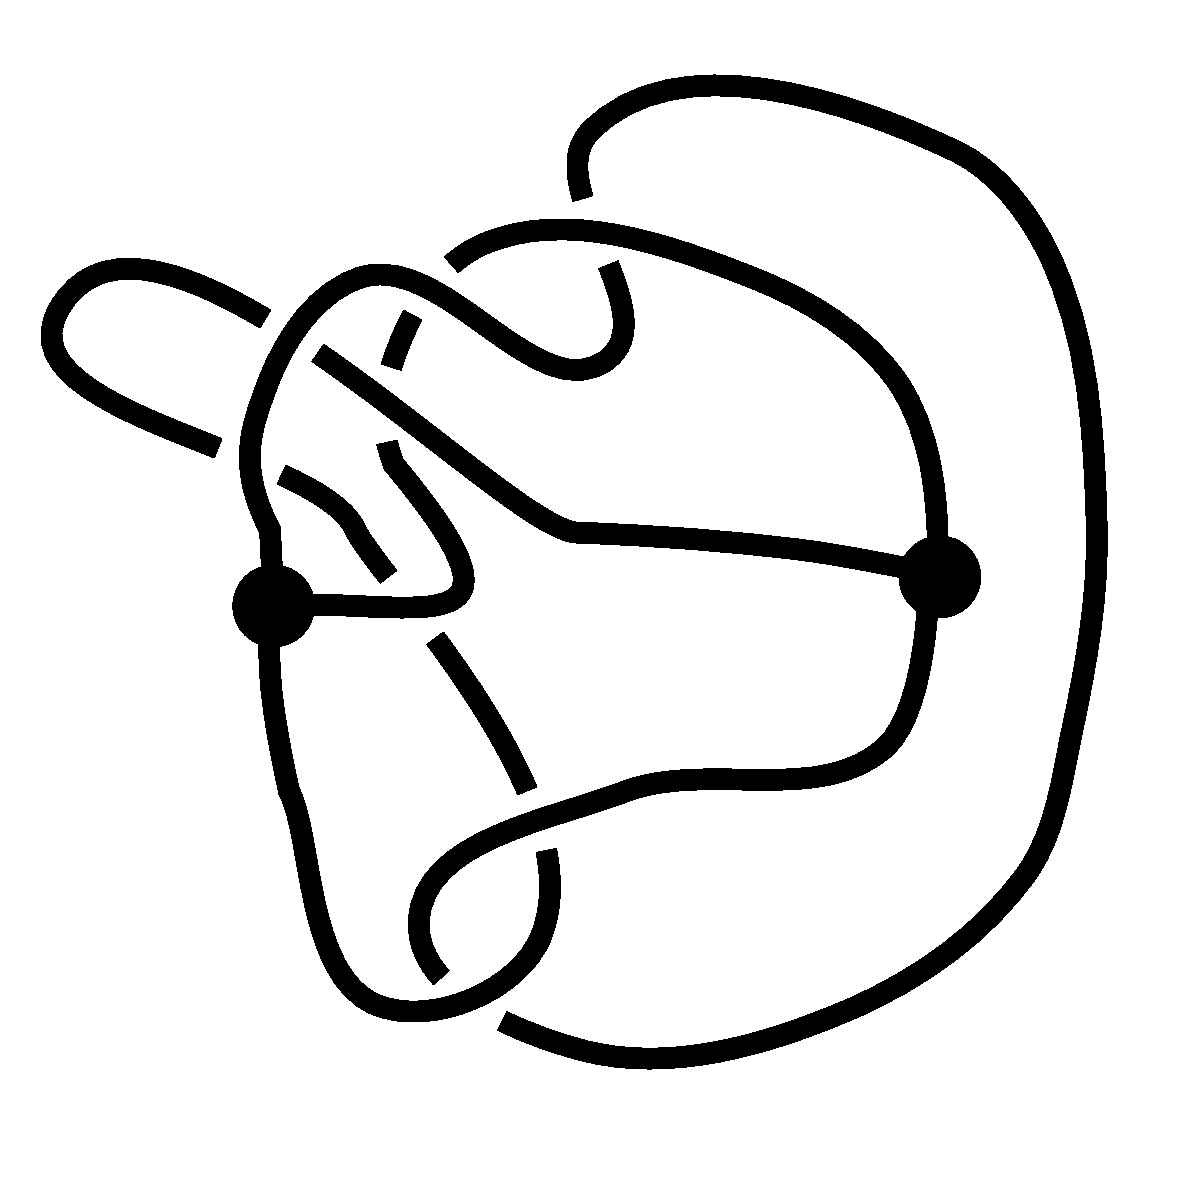
\includegraphics[scale=0.15]{knot_08_b03.pdf}\\
             & \overset{R.III}{\Rightarrow} 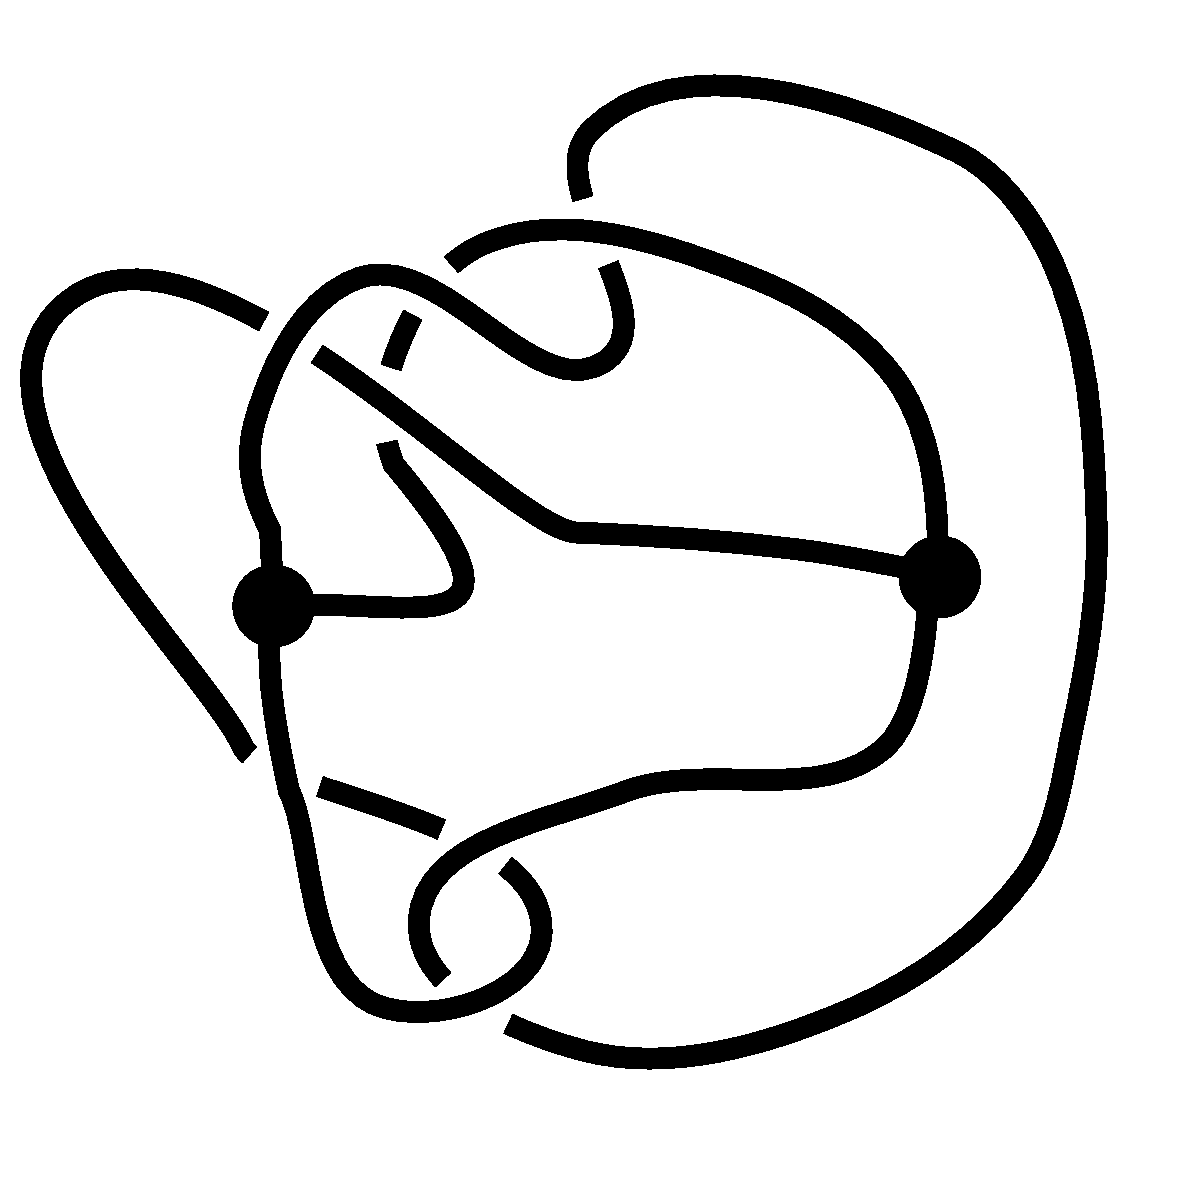
\includegraphics[scale=0.15]{knot_08_b04.pdf}
             & \overset{R.I}{\Rightarrow} 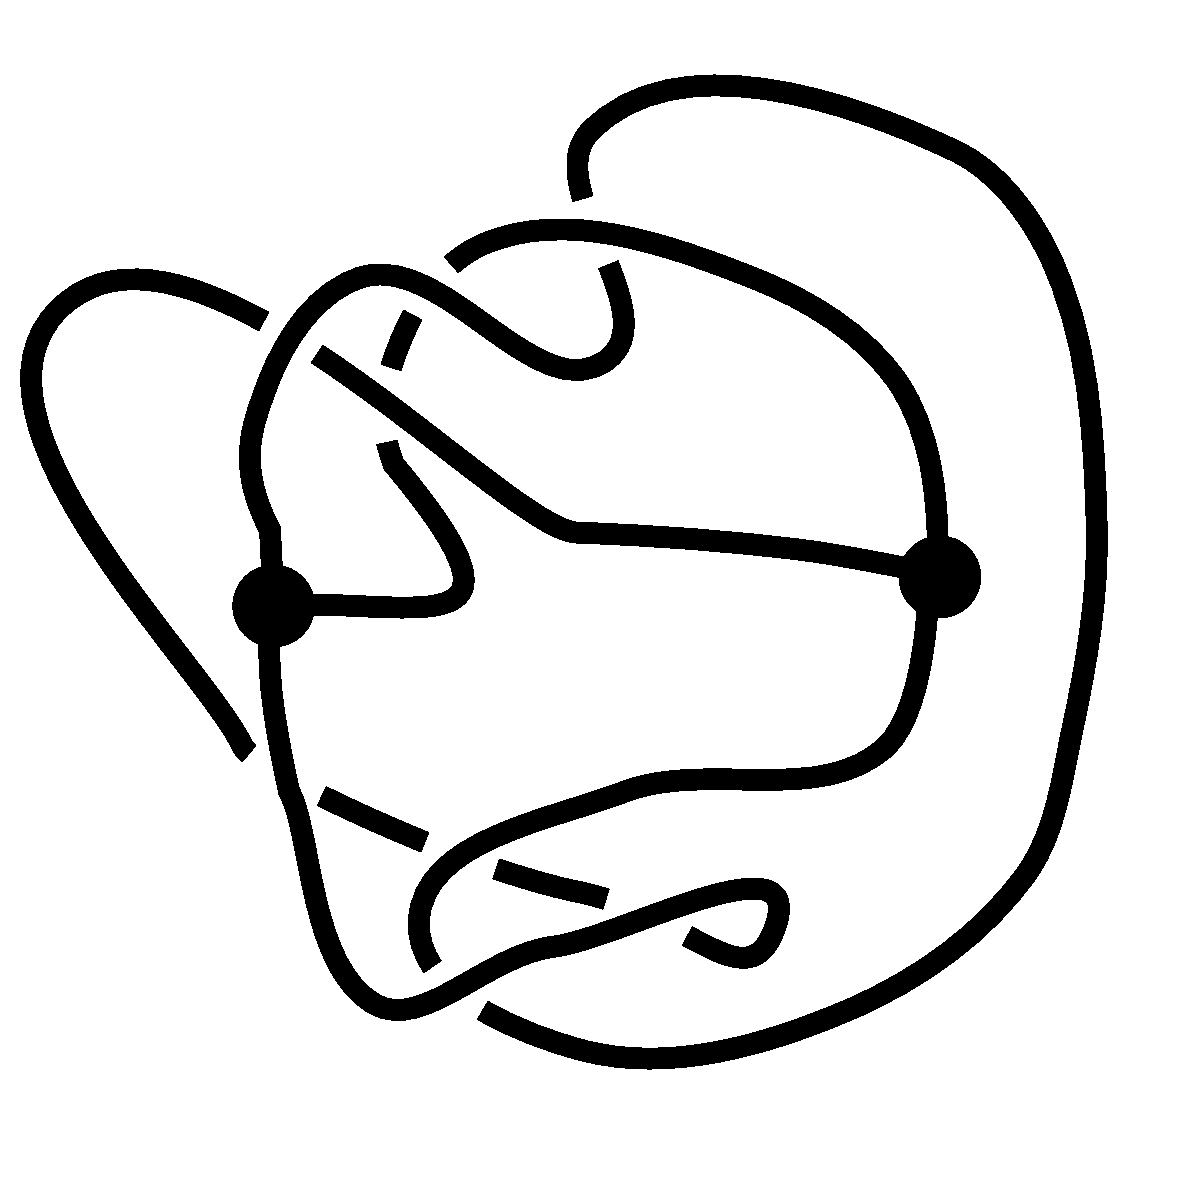
\includegraphics[scale=0.15]{knot_08_b05.pdf}
             & \overset{R.III}{\Rightarrow} \includegraphics[scale=0.15]{knot_08_b06.pdf}\\
             & \overset{R.II}{\Rightarrow} \includegraphics[scale=0.15]{knot_08_b07.pdf}
             & \overset{}{\Rightarrow} \includegraphics[scale=0.15]{knot_08_b08.pdf}
             & \overset{R.III}{\Rightarrow} \includegraphics[scale=0.15]{knot_08_b09.pdf}\\
             & \overset{R.II}{\Rightarrow} \includegraphics[scale=0.15]{knot_08_b10.pdf}
             & \overset{}{\Rightarrow} \tilde{g}(G)
            \end{align}


            \hrulefill

      \end{enumerate}





 \item
      $K_{3,3}$の空間グラフ$f(K_{3,3})$のSimon不変量$\mathcal{L}(f)$を求めよ。

      \dotfill

      各点を結ぶ交点の符号を計算する。
      \begin{enumerate}
       \item
            点1 から 点2
            
            $0$

       \item
            点2 から 点3
            
            $(-1)+(-1) = -2$

       \item
            点3 から 点4
            
            $1 + 1 = 2$

       \item
            点4 から 点5
            
            $0$

       \item
            点5 から 点6
            
            $1+1 = 2$

       \item
            点6 から 点1
            
            $(-1) + (-1) = -2$

       \item
            点1 から 点4
            
            $(-1)+ (-1)+(-1) + 1 + 1+1 + (-1) = -1$

       \item
            点5 から 点2
            
            $(-1)+ 1+1 + 1 + (-1)+(-1) + (-1) = -1$

       \item
            点3 から 点6
            
            $0$
      \end{enumerate}

      以上の9本の辺の交点から求めた符号をあわせる。
      \begin{equation}
       \mathcal{L}(f) = (0 + (-2) + 2 + 0 +2 + (-2) + (-1) + (-1) + 0 )/2 = -1
      \end{equation}

      \hrulefill

      \hrulefill



 \item [\fbox{17}]
      有向グラフ$K_{4},D_{3}$について、
       以下の設問に答えよ。

      \begin{equation}
       \begin{matrix}
        \includegraphics[scale=0.2]{knot_17_K4.pdf} &
       \includegraphics[scale=0.2]{knot_17_D3.pdf}\\
       K_{4} & D_{3}
       \end{matrix}
       \end{equation}

       \begin{enumerate}
        \item
             $K_{4}$の1次元ホモロジー群$H_1(K_{4} ; \mathbb{Z})$
             を求めよ。

             \dotfill

             \begin{align}
              C_{0}(K_{4})
                &= \langle 1,2,3,4 \rangle\\
              C_{1}(K_{4})
                &= \langle e_{1},e_{2},e_{3},e_{4},e_{5},e_{6} \rangle\\
              C_{2}(K_{4})
                &= \langle
                  e_{1}-e_{5}+e_{4}, e_{2}-e_{6}+e_{5},e_{3}-e_{4}+e_{6}
                \rangle
             \end{align}


             \hrulefill
        \item
             $D_{3}$の1次元ホモロジー群$H_1(D_{3} ; \mathbb{Z})$
             を求めよ。

             \dotfill

             \hrulefill
       \end{enumerate}


\end{enumerate}

\hrulefill

\end{document}
